\documentclass{article}
\usepackage{geometry}
 \geometry{
 a4paper,
 total={170mm,257mm},
 left=20mm,
 top=20mm,
 }
\usepackage{graphicx}
\usepackage{array}
\usepackage{setspace}
\usepackage[inkscapeformat=png]{svg}
\usepackage{graphicx}
\usepackage{tabularx}
\usepackage{caption}
\usepackage{subcaption} 
\usepackage{overpic}
\usepackage{tikz}
\usepackage{amsmath}
\usepackage{amssymb} % or \usepackage{amsfonts}
\usepackage{hyperref}
\usepackage{listings}
\usepackage{xcolor}
\usepackage{{booktabs}}
%\usepackage{apacite}
\usepackage{float}
\usepackage{booktabs}
\usepackage{enumitem}
\usepackage[spanish]{babel}
\usepackage[inkscapeformat=png]{svg}
\usepackage{multirow}

\definecolor{codegreen}{rgb}{0,0.6,0}
\definecolor{codegray}{rgb}{0.5,0.5,0.5}
\definecolor{codepurple}{rgb}{0.58,0,0.82}
\definecolor{backcolour}{rgb}{0.95,0.95,0.92}

% macro para la matriz de imágenes
\newcommand*{\addheight}[2][.5ex]{%
  \raisebox{0pt}[\dimexpr\height+(#1)\relax]{#2}%
}

\newcolumntype{M}[1]{>{\centering\arraybackslash}m{#1}}

\lstdefinestyle{mystyle}{
    backgroundcolor=\color{backcolour},   
    commentstyle=\color{codegreen},
    keywordstyle=\color{magenta},
    numberstyle=\tiny\color{codegray},
    stringstyle=\color{codepurple},
    basicstyle=\ttfamily\footnotesize,
    breakatwhitespace=false,         
    breaklines=true,                 
    captionpos=b,                    
    keepspaces=true,                 
    numbers=left,                    
    numbersep=5pt,                  
    showspaces=false,                
    showstringspaces=false,
    showtabs=false,                  
    tabsize=2
}

\lstset{style=mystyle}

% double underscore
\newcommand{\dunsc}{\rule{2\dunder}{0.4pt}} 

\begin{document}
\begin{doublespace}
    \begin{center}
        \Large{\textbf{Instituto Tecnológico de Costa Rica}}
        \bigskip\par\end{center}

    \begin{center}
        Escuela de Ingeniería en Computación.\\
        Programa de Bachillerato en Ingeniería en Computación. \\
        IC6200 - Inteligencia Artificial
        \bigskip\par\end{center}

    \begin{center}
        \Large{\textbf{Trabajo Práctico 1: Redes Neuronales}}\\
        Profesor: Ph. D. Saúl Calderón Ramírez
        \par\end{center}
\end{doublespace}

\begin{doublespace}
    \begin{center}
        \begin{abstract}
            En el presente trabajo práctico se introducirá el concepto de redes neuronales. Consta de 100 puntos distribuidos en 4 secciones. La primera sección tratará sobre la implementación de una red neuronal realimentada, la segunda sección de un clasificador para XOR, la tercera sección de un clasificador de datos en $\mathbb{R}^2$, y la cuarta sección de un clasificador de ataques con datos estructurados.
        \end{abstract}
        \par\end{center}
\end{doublespace}

\begin{center}
    \textbf{Estudiantes} \bigskip{} \\
    \begin{table}[h]
        \begin{center}
            \begin{tabular}{@{}lc@{}}
                José Adrián Amador Ávila    & 2016101574   \\
                Josué Castro Ramírez   & 2020065036 
            \end{tabular}
        \end{center}
    \end{table}
    \vfill{}
    \par\end{center}

\begin{center}
    IS2024\newpage{}
    \par\end{center}

\tableofcontents
\newpage

\section{Implementación de una red neuronal realimentada}

Esta sección detalla como se realizó la implementación de la red a través de una \textit{clase} en el lenguaje de programación Python, la cuál se hizo de la forma más matricial posible con las funciones que brinda la biblioteca \textit{PyTorch}. La presente sección cubre los siguientes contenidos:

\begin{itemize}
    \item Concepto de red neuronal
    \item Clase \texttt{Multi\_layer\_perceptron}
    \item Implementación de la función \texttt{\textit{\rule{0.8em}{.1pt}init\rule{0.8em}{.1pt}()}}
    \item Propagación hacia adelante: función \texttt{\textit{forward()}}
    \item Entrenamiento de la red: función \texttt{\textit{train\_mlp()}}
\end{itemize}



\subsection{Concepto de red neuronal}\label{sec:neural_net}

Las redes neuronales son sistemas de procesamiento de información inspirados en el sistema nervioso y el cerebro de animales y humanos. Están compuestas por una gran cantidad de unidades simples, conocidas como neuronas, que operan en paralelo y se comunican mediante señales de activación a lo largo de conexiones dirigidas \cite{Kruse2016Introduction}. Las redes neuronales son ensamblajes altamente interconectados de elementos simples que cambian de estado cuando su entrada supera un valor umbral específico, lo que permite modelar comportamientos cooperativos y propiedades computacionales similares a las del sistema nervioso \cite{Sompolinsky1988STATISTICAL}.

\begin{figure}[h!]
    \centering
    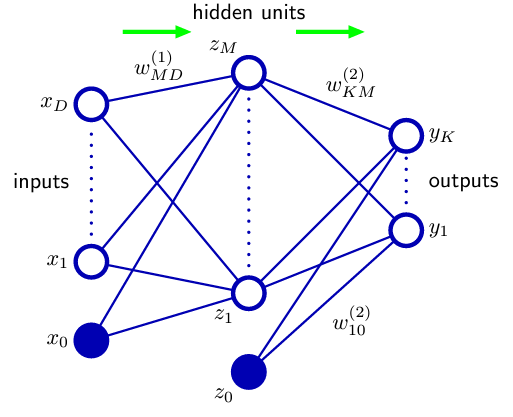
\includegraphics[width=0.5\linewidth]{imgs/neural_network_graph.png}
    \caption{Diagrama de una red neuronal de dos capas (excluyendo la capa de entrada), tomado de \cite{bishop2006pattern}.}
    \label{fig:neuronal_network}
\end{figure} 

Tal como se muestra en la figura \ref{fig:neuronal_network}, una red neuronal es esencialmente un grafo, usualmente de tres capas. Podemos entonces definir cada una de las capas como:

\begin{itemize}
    \item La capa de entrada de $D$ nodos, constituida por los valores $x_1, x_2, x_3,..., x_D$ del arreglo de entrada $\vec{x} \in \mathbb{R}^D$.

    \item La capa oculta de $M$ nodos, constituida por los valores $y_0^{o}, y_1^{o}, y_2^{o},..., y_M^{o}$, en notación vectorial dada por $\vec{y^o} \in \mathbb{R}^M$. Esta capa controla el nivel de generalización de la red (suavidad de la superficie de decisión).
    
    \item La capa de salida, constituida por $K$ nodos $y_1^{s},...,y_K^{s}$, con $\vec{y^s} \in \mathbb{R}^K$, lo cual corresponde al \textbf{número \textit{K} de clases por discriminar}. 
\end{itemize}

\subsubsection{Propagación hacia adelante}\label{sec:forward_details}

Cada una de las capas tiene una matriz de pesos $W^o \in \mathbb{R}^{D \times M}$ y $W^s \in \mathbb{R}^{M \times K}$. La primera matriz de pesos conecta las neuronas de entrada con la capa oculta, y la segunda matriz conecta la capa oculta con la capa de salida. Para cada nodo de la capa oculta, se define el \textbf{peso neto o coeficiente de activación} $p_m^o$, el cual está dado por la combinación lineal de los valores de los nodos de entrada por los pesos de la capa oculta:

\begin{equation}
    p_m^o\left(\vec{x},W^o\right) = \sum_{d=1}^{D}{W_{d,m}^{o} x_d + W_{0,m}^o} \label{eq:p_o_eq},
\end{equation}

\noindent
donde el peso $W_{0,m}^o$ se refiere comúnmente al \textbf{sesgo}, el cual de ignorarse, se puede reescribir la expresión como:

\begin{align*}
    p_m^o\left(\vec{x},W^o\right) = \sum_{d=1}^{D}{W_{d,m}^{o} x_d}
\end{align*}
\noindent
fijando a $x_0=1$, siendo también el \textbf{bias} o \textbf{sesgo}. \\

\noindent
El peso neto $p_m$ es transformado usando una \textbf{función de activación} no lineal y diferenciable:

\begin{equation}
    y_m^o\left(\vec{x},W^o\right) = g^{o}\left(p_m^o\left(\vec{x},W^o\right)\right) \label{eq:y_o_func},
\end{equation}

\noindent
cada uno de los valores de los nodos $\textbf{}y_0^{o}, y_1^{o}, y_2^{o},..., y_M^{o}$, se les llama \textbf{salidas de la capa oculta}. \\

La función de activación $g^o$ denota la condición de una neurona como activada o desactivada ante una entrada específica. Para el caso de este trabajo práctico, se hará uso de la función \textbf{tangente hiperbólica} como función de activación, y está dada por:

\begin{align}
    \tanh(x) &= \frac{e^x - e^{-x}}{e^x + e^{-x}} \label{eq:tanh_fun}\\
    \frac{d}{dx}\tanh(x) &= 1 - \tanh^2(x) \label{eq:tanh_deriv}
\end{align}

Ahora bien, para la capa de salida, siguiendo la figura \ref{fig:neuronal_network}, se define el peso neto para la unidad de salida $k$ como:

\begin{equation}
    p_k^s(\vec{x},W^s) = \sum_{m=0}^{M}{W_{m,k}^s y_m^o} \label{eq:p_s_eq},
\end{equation}

\noindent
donde $y_0^o=1$, siendo la neurona de sesgos en la capa oculta. El peso neto para una neurona en la capa de salida está dada por la combinación lineal de las salidas de la capa oculta por los pesos de la capa de salida. Y de la misma forma, para obtener las salidas de la capa de salida, se pasa cada uno de los pesos netos $p_k^s$ por una función de activación:

\begin{equation}
    y_k^s(\vec{x}, W^s) = g^s(p_k^s(\vec{x}, W^s). \label{eq:y_s_eq}
\end{equation}

\noindent
Si reemplazamos el funcional $y_k^s$ por su definición en la ecuación \ref{eq:p_s_eq}, se tiene que:

\begin{equation}
    y_k^s(\vec{x}, W^s) = g^s\left(\sum_{m=0}^{M}{W_{m,k}^s y_m^o}\right),
\end{equation}
\noindent
y si, de la misma manera reemplazamos $y_m^o$ por su ecuación \ref{eq:y_o_func}, y dentro de esa misma ecuación el funcional $p_m^o$ por su ecuación \ref{eq:p_o_eq}:

\begin{equation}
    y_k^s(\vec{x}, W^o, W^s) = g^s\left( \sum_{m=0}^{M}{W_{m,k}^s g^{o} \left( \sum_{d=1}^{D}{W_{d,m}^{o} x_d + W_{0,m}^o}\right) } + W_{0,k}^s\right). \label{eq:forward_eq}
\end{equation}
\noindent
El proceso de evaluar la ecuación \ref{eq:forward_eq} se le conoce como \textbf{propagación hacia adelante}. \\

\subsubsection{Retropropagación} \label{sec:backpropagation_details}
Después de realizar la propagación hacia adelante, se debe actualizar los pesos de la capa de salida y la capa oculta. Para encontrar mejores pesos que logren minimizar el error, se usa una ténica llamada \textbf{retropropagación} o \textbf{backpropagation}. Para esto se va a utilizar el algoritmo del \textbf{descenso del gradiente}:

\begin{equation}
    \vec{w}(\tau+1) = \vec{w}(\tau) - \alpha\nabla E(\vec{w}(\tau)). \label{eq:grad_des}
\end{equation}
\noindent
Definimos entonces la ecuación del error como:

\begin{equation}
    E(\vec{w}) = \frac{1}{N}\sum_{n=1}^{N}\|y(\vec{x_n},\vec{w}) - \vec{t_n}\|^2, \label{eq:ew_error}
\end{equation}
\noindent
o bien, 

\begin{equation*}
    E(\vec{w}) = \sum_{n=1}^{N}{E_n(\vec{w})},
\end{equation*}
\noindent
con
\begin{equation*}
    E_n(\vec{w}) = \frac{1}{N}\|y(\vec{x_n}, \vec{w}) - \vec{t_n}\|^2.
\end{equation*}

\noindent
\textbf{Capa de salida}
\medskip

Para actualizar los pesos de la\textbf{ capa de salida}, $W^s$, tenemos,

\begin{equation}
    W_{m,k}^s(\tau + 1) = W_{m,k}^s(\tau) - \alpha \nabla W_{m,k}^s(\tau), \label{eq:graddesc_s}
\end{equation}
\noindent
donde, 

\begin{equation}
    \nabla W^s_{m,k}(\tau) = \frac{d}{dW^s_{m,k}}\left(\sum_{n=1}^{N}{E_n(W_{m,k}^s)}\right).
\end{equation}
\noindent
Podemos transformar de igual manera la ecuación de $E_n(\vec{w})$, de la siguiente forma,

\begin{equation*}
    E_n(W^s) = \sum_{k=0}^{K}{E_{k,n}(W^s)},
\end{equation*}
\noindent
con el error por cada unidad de salida k,
\begin{equation*}
    E_{k,n}(W^s) = \frac{1}{N}\left(y_k^s(\vec{x_n}, W^s) - t_{k,n}\right)^2 = \frac{1}{N}\left(g^s(p_{k,n}^s) - t_{k,n}\right)^2.
\end{equation*}
\noindent
Calculando la derivada parcial del error para una muestra $n$ respecto a una entrada de la matriz de pesos $W_{m',k'}^s$, se tiene que:
\begin{equation*}
    \frac{dE_n}{dW_{m',k'}^s} = \frac{d}{dW_{m',k'}^s}\left( \sum_{k=0}^{K}{E_{k,n}(W^s)}\right),
\end{equation*}
\noindent
lo que significa,
\begin{equation}
    \frac{dE_{k,n}}{dW_{m',k'}^s} = \frac{d}{dW_{m',k'}^s}\left( \frac{1}{N}\left(g^s(p_{k',n}^s) - t_{k',n}\right)^2 \right).
\end{equation}
\noindent
Podemos entonces descomponer la derivada parcial usando la regla de la cadena para obtener lo siguiente:
\begin{equation}
    \frac{dE_{k,n}}{dW_{m',k'}^s} = \frac{dE_{k,n}}{dy_{k',n}^s} \frac{dy_{k',n}^s}{dp_{k',n}^s} \frac{dp_{k',n}^s}{dW_{m',k'}^s}. \label{eq:par_deriv_s}
\end{equation}
\noindent
Dado que se está trabajando con la función tangente hiperbólica, $y_{k',n}^s = g^s(p_{k',n}^s) = \tanh(p_{k',n}^s)$, para la cual tenemos su derivada en la ecuación \ref{eq:tanh_deriv}, $\frac{d}{dp_{k',n}^s}\tanh(p_{k',n}^s) = 1 - \tanh^2(p_{k',n}^s)$. Con esto, cada una de las derivadas parciales de la ecuación \ref{eq:par_deriv_s}, se desarrolla de la siguiente manera:
\begin{align}
    \frac{dE_{k,n}}{dy_{k',n}^s} &= \frac{dE_{k,n}}{dy_{k',n}^s}\left( (y_{k',n}^s - t_{k',n})^2 \right) = 2(y_{k',n}^s - t_{k',n}), \\
    \frac{dy_{k',n}^s}{dp_{k',n}^s} &= 1 - \tanh^2(p_{k',n}^s) = 1 - (y_{k',n}^s)^2, \\
    \frac{dp_{k',n}^s}{dW_{m',k'}^s} &= \frac{d}{dW_{m',k'}^s} \left( \sum_{m=0}^{M} W_{m,k'}^s y_{m,n}^o \right) = y_{m',n}^o,
\end{align}
\noindent
por lo cual, la derivada de la ecuación \ref{eq:par_deriv_s}, se puede expresar como:
\begin{equation}
    \frac{dE_{k',n}}{dW_{m',k'}^s} = \left(2(y_{k',n}^s - t_{k',n})\right) \left(1 - (y_{k',n}^s)^2\right) y_{m',n}^o, \label{eq:par_der_s_full}
\end{equation}
\noindent
y podemos tomar, para una muestra $n$, el \textit{delta} o \textit{cambio de aprendizaje} $\delta_k^s$ como:
\begin{equation}
    \delta_{k',n}^s = \left(2(y_{k',n}^s - t_{k',n})\right) \left(1 - (y_{k',n}^s)^2\right). \label{eq:delta_s_equ}
\end{equation}
\noindent
De esta manera, la actualización del peso $W_{m',k'}^s$ vendría dada, según la ecuación \ref{eq:graddesc_s} por cada muestra como:
\begin{equation}
    W_{m',k'}^s(\tau + 1) = W_{m',k'}^s(\tau) - \alpha \nabla W_{m',k'}^s(\tau), \label{eq:grad_desc_s_final}
\end{equation}
\noindent
con
\begin{equation*}
    \nabla W_{m',k'}^s(\tau) = \delta_{k',n}^{s}y_{m',n}^o.
\end{equation*}

\noindent
\textbf{Capa oculta}
\medskip

Por otro lado, para actualizar los pesos de la \textbf{capa oculta} $W^o$, se desarrollará de forma similar, la ecuación:
\begin{equation}
    W_{d',m'}^o(\tau + 1) = W_{d',m'}^o(\tau) - \alpha \nabla W_{d',m'}^o(\tau), \label{eq:graddesc_o}
\end{equation}
\noindent
donde,
\begin{equation*}
    W_{d',m'}^o(\tau) = \frac{d}{dW_{d',m'}^o}\left( \sum_{n=1}^{N}{E_n(W_{d',m'}^o)} \right).
\end{equation*}
\noindent
Tenemos que el error por cada unidad $k$ de la capa de salida:

\begin{align*}
    E_{k,n}(W^o) &= \frac{1}{N}(y_{k}^s(\vec{x}_n, W^o) - t_{k,n})^2 = \frac{1}{N}(y_{k}^s(p_k^s(\vec{x}_n, W^o)) - t_{k,n})^2 \\
    &= \frac{1}{N}\left( g^s\left( \sum_{m=0}^{M}{W_{m,k}^s g^o \left( \sum_{d=1}^{D}{W_{d,m}^o x_d} \right) } \right) - t_{k,n}\right)^2.
\end{align*}
\noindent
Por lo tanto, podemos descomponer la derivada del error usando la regla de la cadena, como:
\begin{equation}
    \frac{dE_{k,n}}{dW_{d',m'}^o} = \frac{dE_{k,n}}{dy_{k,n}^s} \frac{dy_{k,n}^s}{dp_{k,n}^s}  \frac{dp_{k,n}^s}{dy_{m',n}^o} \frac{dy_{m',n}^o}{dp_{m',n}^o} \frac{dp_{m',n}^o}{dW_{d',m'}^o}. \label{eq:par_deriv_o}
\end{equation}
\noindent
Algo importante a tomar en cuenta es que, un cambio en la capa oculta ocasiona un cambio en el error de todas las unidades en la capa de salida, por lo que entonces:
\begin{equation*}
     \frac{dE_{n}}{dW_{d',m'}^o} = \sum_{k=0}^{K}{\frac{dE_{k,n}}{dW_{d',m'}^o}} = \sum_{k=0}^{K}{ \left( \frac{dE_{k,n}}{dy_{k,n}^s} \frac{dy_{k,n}^s}{dp_{k,n}^s}  \frac{dp_{k,n}^s}{dy_{m',n}^o} \right) }  \frac{dy_{m',n}^o}{dp_{m',n}^o} \frac{dp_{m',n}^o}{dW_{d',m'}^o}.
\end{equation*}
\noindent
Y sus derivadas parciales dadas por:
\begin{align}
    &\frac{E_{k,n}}{dy_{k,n}^s} = 2(y_{k,n}^s - t_{k,n}) \\
    &\frac{dy_{k,n}^s}{dp_{k,n}^s} = 1 - \tanh^2(p_{k,n}^s) =  1 - (y_{k,n}^s)^2 \\
    &\frac{dp_{k,n}^s}{dy_{m',n}^o} = W_{m',k}^s \\
    &\frac{dy_{m',n}^o}{dp_{m',n}^o} = 1 - \tanh^2(p_{m',n}^o) = 1 - (y_{m',n}^o)^2 \\
    &\frac{dp_{m',n}^o}{dw_{d',m'}^o} = x_{d'},
\end{align}
\noindent
y así, la derivada parcial del error respecto a un peso específico, para una muestra $n$, está dada por:
\begin{equation}
    \frac{dE_n}{dW_{d',m'}^o} = \sum_{k=0}^{K}{ \left( (2(y_{k,n}^s - t_{k,n})) (1 - (y_{k,n}^s)^2) (W_{m',k}^s) \right) } (1 - (y_{m',n}^o)^2) x_{d'}. \label{eq:outputlayer_der_error}
\end{equation}
\noindent
Se había definido en la ecuación \ref{eq:delta_s_equ}, el $\delta_{k,n}^s$ para la capa de salida, y este término se puede observar en la ecuación \ref{eq:outputlayer_der_error}, por ello, podemos definir el delta en la capa oculta como:
\begin{equation}
    \delta_{m',k}^o = \left( \sum_{k=0}^{K} \delta_{k,n}^sW_{m',k}^s\right) (1- (y_{m',n}^o)), \label{eq:delta_o_equ}
\end{equation}
\noindent
y por ende, para la ecuación \ref{eq:graddesc_o}, $ W_{d',m'}^o(\tau + 1) = W_{d',m'}^o(\tau) - \alpha \nabla W_{d',m'}^o(\tau)$ , se define:
\begin{equation*}
    \nabla W_{d',m'}^o = \delta_{m',n}^{o}x_{d'}.
\end{equation*}

De esta manera, podemos actualizar los pesos de la capa de salida y oculta, usando las ecuaciones \ref{eq:grad_desc_s_final} y \ref{eq:graddesc_o}, respectivamente.


\newpage
\subsection{Clase \texttt{Multi\_layer\_perceptron}}

Como se detalló al inicio de este informe, se decide definir una \textit{clase} en el lenguaje de programación Python para abordar la implementación de la red neuronal realimentada, a continuación, en la figura \ref{fig:classes_diagram} se presenta un diagrama de clases que muestra los atributos y métodos asociados a la clase de la red, así como su relación con la clase \textit{TestMultiLayerPerceptron}, la cuál fue definida para realizar las respectivas pruebas unitarias la clase principal; para dicha labor se utilizará la biblioteca \texttt{unittest}.

\begin{figure}[h!]
    \centering
    \includesvg[width=0.6\textwidth]{imgs/classes.svg}
    \caption{Diagrama de las clases implementadas.}
    \label{fig:classes_diagram}
\end{figure} 

\subsection{Implementación de la función \texttt{\textit{\rule{0.8em}{.1pt}init\rule{0.8em}{.1pt}}()}}\label{sec:_init_}

Esta función es la encargada de inicializar un perceptrón multicapa, debe inicializar los pesos de la capa oculta y salida de manera completamente aleatoria en un rango entre $-1$ y $1$. Se debe colocar la neurona de entrada extra que representa el \textit{bias} ($D+1$), así como la neurona \textit{bias} ($M+1$) en la capa oculta, en donde sus pesos se representan como \textit{NaN}, por el hecho de no tener conexiones con las neuronas de la capa de entrada. Para su implementación se tomaron en cuenta las siguientes indicaciones: 

\begin{itemize}
    \item \texttt{neurons\_per\_layer} es un arreglo con las neuronas por cada capa, de la forma [\textit{D, M, K}], con \textit{D} las neuronas de entrada, \textit{M} las neuronas en la capa oculta, y \textit{K} las neuronas de la capa de salida.

    \item \texttt{alpha} es el coeficiente de aprendizaje \(\alpha\).

    \item \texttt{gamma} es el coeficiente de momentum \(\gamma\).

    \item \texttt{max\_weights} es el valor máximo que puede tomar cualquiera de los pesos en las dos capas.
\end{itemize}

Otro punto a tomar en cuenta según las indicaciones del trabajo práctico, es que se puede guardar como atributos de clase los pesos netos de la capa oculta y salida ($P^o, P^s$), los deltas ($\delta^o, \delta^s$), así como los tamaños para cada capa ($D, M, K$), los cuáles son definidos en la figura \ref{fig:classes_diagram}. \\


\subsubsection{Código}
Ahora bien, como se puede observar en la figura \ref{code:_init_}, se tiene la implementación, con algunas omisiones, de lo mencionado anteriormente.

% texcl=true : Permite usar tildes
\begin{figure}[h!]
\begin{lstlisting}[language=Python, texcl=true] 
def __init__(self, neurons_per_layer, alpha = 0.01, gamma = 0.9, max_weights = 1):
    # Número de neuronas por capa
    self.neurons_per_layer = neurons_per_layer
    self.D, self.M, self.K = neurons_per_layer
        
    # Neuronas de sesgo
    self.D += 1
    self.M += 1
    
    self.alpha = alpha
    self.gamma = gamma
    self.max_weights = max_weights
    
    # Inicialización de pesos de forma aleatoria dentro del rango permitido
    self.W_o = (torch.rand(self.D, self.M) * 2) - 1
    self.W_o = torch.min(self.W_o, torch.tensor(max_weights))
    
    self.W_s = (torch.rand(self.M, self.K) * 2) - 1
    self.W_s = torch.min(self.W_s, torch.tensor(max_weights))
    
    # Colocamos la neurona de sesgos en la capa oculta
    self.W_o[:, 0] = torch.nan
    
    # Inicialización de los valores de momentum para cada conjunto de pesos
    self.momentum_W_o = torch.zeros_like(self.W_o)
    self.momentum_W_s = torch.zeros_like(self.W_s)
\end{lstlisting}
    \caption{Implementación en código de la función \textit{\rule{0.8em}{.1pt}init\rule{0.8em}{.1pt}()}}
    \label{code:_init_}
\end{figure}



\newpage
\subsubsection{Pruebas unitarias: \textit{\rule{0.8em}{.1pt}init\rule{0.8em}{.1pt}()}}

A continuación, se detalla la prueba de inicialización de la clase del perceptrón multicapa, la cuál busca comprobar la correcta creación del objeto, validando los siguientes aspectos:

\begin{itemize}
    \item \textbf{Límites válidos:} Validar que la capa de pesos no exceda el límite establecido por el atributo \texttt{max\_weights.}

    \item \textbf{Dimensiones válidas:} Validar que las dimensiones de las capas de pesos sea la correcta, $D \times M$ para la capa oculta y $M \times K$ para la de salida.

    \item \textbf{Columna de sesgo correcta:} Validar que la columna del sesgo sea correctamente inicializada. \\
\end{itemize}

\noindent
\textbf{Datos de entrada}
\label{inputs}
\\
Para efectos de esta prueba se definirá un único perceptrón multicapa, se llamará a dicho objeto como \texttt{TESTED\_MLP}, del cual se muestran algunos de sus atributos a continuación:

\begin{itemize}
    \item \texttt{neurons\_per\_layer} = \{3, 3, 2\}.
    \item \texttt{alpha} = 0.01.
    \item \texttt{gamma} = 0.9.
    \item \texttt{max\_weights} = 0.5.
    
    \item \texttt{W\_o} = \{ una matriz aleatoria $W^{o}\in\mathbb{R}^{D \times M}$ $|$ $\forall x \in W^{o} :$ \texttt{-max\_weights} $<= x <=$ \texttt{max\_weights}\}.
    
    \item \texttt{W\_s} = \{ una matriz aleatoria $W^{s}\in\mathbb{R}^{M \times K}$ $|$ $\forall x \in W^{s} :$ \texttt{-max\_weights} $<= x <=$ \texttt{max\_weights}\}.    
\end{itemize}


\noindent
\textbf{Resultados esperados}
\\
Para esta prueba, se espera que una inicialización correcta del perceptrón, más específicamente, se espera que las capas de peso tengan correctamente asignadas las dimensiones que se establecen en el atributo \texttt{neurons\_per\_layer}. Es decir, de la siguiente forma:

\begin{itemize}
    \item $W^{o}\in\mathbb{R}^{4 \times 4}$, recordando que fue agregada la columna de sesgo, por eso se suma 1 a $D$ y $M$.
    \item $W^{s}\in\mathbb{R}^{4 \times 2}$
\end{itemize}

\noindent
Además, se debe validar que los valores aleatorios de las capas de peso estén acotados en un rango establecido,, que en este caso es [-0.5, 0.5]. Y por último, se espera que la capa oculta de pesos tenga correctamente inicializada la columna del sesgo con valores NaN en la primer columna.\\

\noindent
\textbf{Resultados obtenidos}
\\
A continuación en el \textit{Cuadro \ref{tab:init_test}} se observan los datos obtenidos al inicializar el objeto \textbf{\texttt{TESTED\_MLP}}, además se detalla en la última columna las dimensiones obtenidas de las respectivas capas de pesos.

\begin{table}[htbp]
\centering
\resizebox{\textwidth}{!}{%
\begin{tabular}{@{}cccc@{}}
\toprule
\textbf{Datos de entrada} & \textbf{W\_o obtenido} & \textbf{W\_s obtenido} & \textbf{\begin{tabular}[c]{@{}c@{}}Dimensiones\\obtenidas\end{tabular}} \\ \midrule
    \texttt{TESTED\_MLP}
    & \begin{tabular}[c]{@{}c@{}}
        $\left[\begin{array}{cccc}
        NaN & \textbf{-0.5000} & -0.3958 & 0.0390\\
        NaN & 0.4139 & -0.3631 & -0.3337\\
        NaN & 0.1877 & 0.1377 & \textbf{0.5000}\\
        NaN & 0.3099 & 0.4860 & \textbf{-0.5000}\\
        \end{array}\right]$
    \end{tabular}

    & \begin{tabular}[c]{@{}c@{}}
        $\left[\begin{array}{cc}
        -0.0893 & -0.4776\\
        \textbf{-0.5000} & -0.2983\\
        \textbf{0.5000} & -0.0185\\
        -0.4422 &  \textbf{0.5000}
        \end{array}\right]$
    \end{tabular}
    
    & \begin{tabular}[c]{@{}c@{}}
        $W^{o}\in\mathbb{R}^{4 \times 4}$ \\
        $W^{s}\in\mathbb{R}^{4 \times 2}$
    \end{tabular} \\ \bottomrule
    
\end{tabular}%
}
\caption{Resultados obtenidos de la prueba unitaria de la función \textit{\rule{0.8em}{.1pt}init\rule{0.8em}{.1pt}()}}
\label{tab:init_test}
\end{table}


\noindent
De los anteriores resultados obtenidos en el \textit{Cuadro \ref{tab:init_test}}, se puede evidenciar que:

\begin{itemize}
    \item Se resaltan \textbf{en negrita} los valores mínimos y máximos obtenidos en las capas de pesos, los cuales respetan estar en el rango establecido.
    \item Las dimensiones de las capas de peso son correctas, y respetan el número de neuronas que entra por parámetro de inicialización.
    \item El \texttt{W\_o} obtenido cumple que su primer columna es puros datos NaN, por ende, la prueba es aprobada satisfactoriamente.
\end{itemize}

\newpage
\subsection{Propagación hacia adelante: función \texttt{\textit{forward(X)}}}

Partiendo de lo explicado en la sección \ref{sec:neural_net} y la ecuación \ref{eq:forward_eq}, se puede entonces implementar la propagación hacia adelante, no obstante, primero se debe convertir los cálculos a su forma matricial. En primer lugar, se tiene la matriz de entrada $X$, donde cada fila es un vector de observaciones, de modo $\vec{x}_1, \vec{x}_2,...,\vec{x}_D \in \mathbb{R}^{NxD}$. Del mismo modo, se definió que la matriz de pesos para la capa oculta está dada por $W^o \in \mathbb{R}^{DxM}$, por lo tanto para obtener la matriz de pesos netos $P^o$ de la capa oculta:

\begin{equation}
    P^o = X \cdot W^o,
\end{equation}

\noindent
de manera que $P^o \in \mathbb{R}^{NxM}$. Y esta matriz de pesos netos para la capa oculta se pasa a la función de activación \textbf{tangente hiperbólica}:

\begin{equation}
    Y^o = \tanh{(P^o)},
\end{equation}
\noindent
dando como resultado la salida de la capa oculta $Y^o \in \mathbb{R}^{NxM}$.

Luego de esto, como la primera columna de la matriz de pesos $W^o$ es inicializada con \textit{NanN}, la matriz $Y^o$ también contiene \textit{NaN} en su primer columna, por ello se cambian por $1$, y ya se podría continuar con el siguiente paso, el cual es realizar la combinación lineal que genera los pesos netos $P^s$.

Se sabe que la matriz de pesos para la capa de salida está dada por $W^s \in \mathbb{R}^{MxK}$, y para obtener $P^s$ se debe realizar la combinación lineal entre las salidas de la capa oculta $Y^o$ por los pesos $W^s$, tal que,

\begin{equation}
    P^s = Y^o \cdot W^s,
\end{equation}
\noindent
donde $P^s \in \mathbb{R}^{NxK}$. Y por último, se pasan los pesos netos de la capa de salida por la función de activación, dando como resultado las salidas de la capa de salida,

\begin{equation}
    Y^s = \tanh{(P^s)},
\end{equation}

\noindent
de tal manera que, $Y^s \in \mathbb{R}^{NxK}$. Por medio de estas ecuaciones se puede entonces hacer la implementación de la función \texttt{forward(X)}, tal y como se muestra en la figura \ref{code:fwd}.
%% Esto de acá lo veo redundante, ya su explicación de arrbia está más coompleta xd

% Esta función actualiza los pesos netos y salidas de cada capa, usando el algoritmo de propagación hacia adelante. Se recibe como entrada la matriz \textit{X} con \textit{n} observaciones de entrada. Recordando, se estableció que la red debe utilizar la función \textit{tangente hiperbólico} como función de activación para las capas.

\begin{figure}[htbp]
\begin{lstlisting}[language=Python, texcl=true]
def calculate_tanh(p):
    return (torch.exp(p) - torch.exp(-p)) / (torch.exp(p) + torch.exp(-p))

def forward(self, X):
    # Calcular la salida de la capa oculta
    self.P_o = X.mm(self.W_o)
    self.Y_o = calculate_tanh(self.P_o)

    # Reemplazar valores NaN con 1's
    tmpY_o = self.Y_o
    tmpY_o[torch.isnan(tmpY_o)] = 1.

    # Calcular la salida de la capa de salida
    self.P_s = tmpY_o.mm(self.W_s)
    self.Y_s = calculate_tanh(self.P_s)

    # Retornar la salida de la capa de salida
    return self.Y_s
\end{lstlisting}
    \caption{Implementación en código de la función forward}
    \label{code:fwd}
\end{figure}
    

\subsubsection{Pruebas unitarias: \textit{forward(X)}}

A continuación, se detalla la prueba de la función \texttt{forward}, la cuál busca comprobar el correcto comportamiento de la función, validando los siguientes aspectos:

\begin{itemize}
    \item \textbf{Dimensiones correctas:} Validar que las dimensiones de la capa de salida sea la correcta, es decir, $M \times K$.

    \item \textbf{Ausencia de valores NaN:} Validar que la capa de salida no tenga valores en NaN.
    
    \item \textbf{Rangos correctos:} Validar que la capa de salida tenga sólo valores entre -1 y 1, . \\
\end{itemize}

\noindent
\textbf{Datos de entrada} 
\\
Al igual que en la \textit{Sección \ref{inputs}}, se utilizará el objeto \texttt{TESTED\_MLP} para realizar las pruebas, teniendo los mismos parámetros de inicialización. Además se utilizará una matriz aleatoria de neuronas de entrada $X$, la cuál es de la forma $X \in \mathbb{R}^{5 \times 2}$. \\


\noindent
\textbf{Resultados esperados}
\\
Para esta prueba, se espera el correcto funcionamiento de la función \textit{forward}, más específicamente, se espera que la capa de salida tenga las dimensiones $N \times K$ correctas, las cuáles son en este caso $5 \times 2$. Además, se espera que en la capa de salida presente ausencia de valores NaN, y que dichos valores estén en el rango [-1, 1], el cuál es dado por la función de activación tangente hiperbólico. \\

\noindent
\textbf{Resultados obtenidos}
\\
A continuación en el \textit{Cuadro \ref{tab:fwd_test}} se observan los datos obtenidos al inicializar el objeto \textbf{\texttt{TESTED\_MLP}}, además se detalla en la última columna las dimensiones obtenidas de las respectivas capas de pesos.

\begin{table}[h]
\centering

\begin{tabular}{@{}ccc@{}}
\toprule
\textbf{Datos de entrada} & \textbf{Y\_s obtenido} & \textbf{Dimensiones obtenidas} \\ \midrule
    \begin{tabular}[c]{@{}l@{}}- \texttt{TESTED\_MLP}\\  - $X \in \mathbb{R}^{5 \times 2}$\end{tabular}
    & \begin{tabular}[c]{@{}c@{}}
        $\left[\begin{array}{cc}
        -0.3239 & -0.8920\\
        0.3210 & -0.0904\\
        0.1181 & -0.6024\\
        0.0111 & -0.7714\\
        0.0207 & -0.8440
        \end{array}\right]$
    \end{tabular}
    & $Y^{s} \in \mathbb{R}^{5 \times 2}$ \\ \bottomrule
\end{tabular}%
 
\caption{Resultados obtenidos de la prueba unitaria de la función \textit{forward(X)}}
\label{tab:fwd_test}
\end{table}

\noindent
De los anteriores resultados obtenidos en el \textit{Cuadro \ref{tab:fwd_test}}, se puede evidenciar que:

\begin{itemize}
    \item Las dimensiones obtenidas en \texttt{Y\_s} son correctas.
    \item La capa de salida no cuenta con valores NaN.
    \item Los valores de la capa de salida están dentro del rango de la función de activación.
\end{itemize}

\subsection{Entrenamiento de la red: función \texttt{train\_mlp()}}

En la presente sección, se explica cómo se logra el entrenamiento de la red. Dicho proceso se realiza a través de la función \texttt{train\_mlp()}, la cuál se encarga de entrenar al perceptrón multicapa mediante un algoritmo basado en el descenso del gradiente y usará como función de activación la función tangente hiperbólica para las capas. Esta función se construirá a partir de las siguientes funciones:

\begin{itemize}
    \item \texttt{get\_error(X, T):} La cuál calcula el error medio cuadrático para un conjunto de salidas y objetivos.
    
    \item \texttt{back\_propagate\_deltas(X, T):} La cuál calcula los deltas de error para las capas oculta y de salida.

    \item \texttt{update\_weights(X, T):} La cuál actualiza los pesos de las capas según los deltas de la red.
\end{itemize}

\noindent
Antes de detallar cómo se realiza el entrenamiento, se procede a explicar cómo se construyen cada una de las funciones que componen a la función \texttt{train\_mlp()}.

\subsubsection{Función \textit{get\_error(X, T)}}

La función de error de Cuadrados Medios o Mean Squared Error (MSE) es un criterio estadístico usado para medir la calidad de estimadores y modelos predictivos. El MSE calcula la media de los cuadrados de las diferencias entre los valores estimados y los reales, proporcionando una medida cuantitativa de la precisión del modelo. Es especialmente útil en contextos donde las diferencias grandes entre los valores predichos y los reales son particularmente indeseables, ya que el elevar al cuadrado los errores hace que estas diferencias tengan un impacto mayor en el MSE. En los materiales del curso, vimos la siguiente definición de la función de error:


\begin{equation}
E(\vec{w})=\frac{1}{N}\sum_{n=1}^{N}\left\Vert y(\vec{x_{n},}\vec{w})-\vec{t_{n}}\right\Vert ^{2} \label{eq:MSE}
\end{equation}


\noindent
En base a ello, se define en código la función de la siguiente manera:

\begin{figure}[htbp]
\begin{lstlisting}[language=Python, texcl=true]
def get_error(self, Y_s, T):
    # Calcular el error utilizando la función de error E(w)
    error = torch.sum(torch.norm(Y_s - T, p=2, dim=1)**2) * (1 / Y_s.shape[0])
    return error.item()\end{lstlisting}
    \caption{Implementación en código de la función de error $E(\Vec{w})$}
    \label{code:MSE}
\end{figure}

\newpage
\subsubsection{Función \textit{backpropagate\_deltas(X, T)}}

La retro-propagación, o propagación hacia atrás, es un método fundamental en el entrenamiento de redes neuronales artificiales. Este método consiste en ajustar los pesos de las conexiones de la red de manera eficiente, calculando los gradientes de una función de error respecto a los pesos de la red mediante una propagación hacia atrás desde la capa de salida hasta la de entrada. Este proceso permite que la red aprenda de los errores cometidos en predicciones anteriores, ajustándose para mejorar en iteraciones futuras. 
\medskip

\noindent
\textbf{Ecuaciones de los deltas}
\medskip

Tomando como base las ecuaciones \ref{eq:delta_s_equ} y \ref{eq:delta_o_equ}, podemos calcular los $\delta$ de cada una de las capas. Recordando que el $\delta_{k,n}^s = \left(2(y_{k',n}^s - t_{k',n})\right) \left(1 - (y_{k',n}^s)^2\right)$, para un $k$ en específico dado una muestra $n$, podemos convertir la ecuación a su versión matricial de la siguiente manera:
\begin{equation}
     \delta^{s} = 2(Y^{s} - T) \times (1 - (Y^{s})^{2}),\label{eq:delta_s_matrix}
\end{equation}
\noindent
como se mencionó anteriormente, $Y^s \in \mathbb{R}^{NxK}$, además, $T \in \mathbb{R}^{NxK}$, por lo tanto, $\delta^s \in \mathbb{R}^{NxK}$; y de manera similar, la ecuación $\delta_{m',k}^o = \left( \sum_{k=0}^{K} \delta_{k,n}^sW_{m',k}^s\right) (1- (y_{m',n}^o))$, 

\begin{equation}
    \delta^{o} = (\delta^{s} \cdot (W^{s})^{T}) \times (1 - (Y^{o})^{2}), \label{eq:delta_o_matrix}
\end{equation}
\noindent
como $\delta^s \in \mathbb{R}^{NxK}$ y $W^s \in \mathbb{R}^{MxK}$, se debe tomar la transpuesta de la matriz $W^s$ para dicha operación, dando como resultado una matriz de tamaño $NxM$, lo cual coincide con el tamaño de $Y^o$, por lo tanto se tiene que $\delta^o \in \mathbb{R}^{NxM}$.
\medskip

\noindent
\textbf{Código}
\medskip

Usando entonces las ecuaciones \ref{eq:delta_s_matrix} y \ref{eq:delta_o_matrix}, se implementa el código mostrado en la figura \ref{code:deltas}.

\begin{figure}[htbp]
\begin{lstlisting}[language=Python, texcl=true]
def backpropagate_deltas(self, X, T):
    # Calcular los deltas de la capa de salida
    self.delta_s = (2 * (self.Y_s - T)) * (1 - (self.Y_s**2))
    
    # Calcular los deltas de la capa oculta
    self.delta_o = self.delta_s.mm(self.W_s.t()) * (1 - (self.Y_o**2))
    return\end{lstlisting}
    \caption{Implementación en código de la función \textit{backpropagate\_deltas}}
    \label{code:deltas}
\end{figure}


\subsubsection{Función \textit{update\_weights(X, T)}}

Para actualizar los pesos de ambas capas se va hacer uso de las ecuaciones \ref{eq:delta_s_matrix} y \ref{eq:delta_o_matrix}, podemos entonces transformar las ecuaciones de los gradientes para los pesos de las dos capas, definidas en las ecuaciones \ref{eq:grad_desc_s_final} y \ref{eq:graddesc_o}, en su forma matricial como:

\begin{equation}
    W^s(\tau + 1) = W^s(\tau) - \alpha \nabla W^s(\tau), \label{eq:grad_s_matrix}
\end{equation}
\noindent
con $\nabla W^s(\tau) = (Y^o)^T \cdot \delta^s$, colocando primera la transpuesta de $Y^o$, dado que $Y^o \in \mathbb{R}^{NxM} \implies (Y^o)^T \in \mathbb{R}^{MxN}$ y $\delta^s \in \mathbb{R}^{NxK}$, por lo que $\nabla W^s(\tau) \in \mathbb{R}^{MxK}$, y en general dando un resultado correspondiente al tamaño de la matriz de pesos de la capa de salida. De la misma forma, tenemos entonces, 
\begin{equation}
    W^o(\tau + 1) = W^o(\tau) - \alpha \nabla W^o(\tau), \label{eq:grad_o_matrix}
\end{equation}
\noindent
con $\nabla W^o(\tau) = X^T \cdot \delta^o$, donde de manera similar a lo anterior, se coloca primero la transpuesta de la matriz de entradas $X$, ya que, $X \in \mathbb{R}^{NxD} \implies X^T \in \mathbb{R}^{DxN}$ y $\delta^o \in \mathbb{R}^{NxM}$, por lo que $\nabla W^o(\tau) \in \mathbb{R}^{DxM}$, y en general, siendo el tamaño correspondiente a la matriz de pesos de la capa oculta. 
\medskip

Ahora bien, en el proyecto se hizo la implementación del \textbf{gradiente con momentum}, de lo cual la única modificación es usar el parámetro $\gamma$. Para ello simplemente se crean dos matrices del mismo tamaño de las matrices de pesos tanto para la capa oculta y salida, se multiplica el coeficiente de momentum $\gamma$ a esas matrices y se suma el gradiente de los pesos $W$ con el coeficiente de aprendizaje $\alpha$. Esto y las ecuaciones \ref{eq:grad_s_matrix} y \ref{eq:grad_o_matrix}, se ven reflejadas en la implementación en código de la figura \ref{code:update}. 

\begin{figure}[htbp]
\begin{lstlisting}[language=Python, texcl=true]
def update_weights(self, X, T):
    # Calcular los gradientes para los pesos
    dW_o = X.t().mm(self.delta_o)
    dW_s = self.Y_o.t().mm(self.delta_s)

    # Aplicar momentum
    self.momentum_W_o = self.gamma * self.momentum_W_o + self.alpha * dW_o
    self.momentum_W_s = self.gamma * self.momentum_W_s + self.alpha * dW_s

    # Actualizar los pesos
    self.W_o -= self.momentum_W_o
    self.W_s -= self.momentum_W_s
    return\end{lstlisting}
    \caption{Implementación en código de la función \textit{update\_weights}}
    \label{code:update}
\end{figure}

\subsubsection{Función \textit{train\_mlp()}}

Para esta función, se hace uso de las funciones explicadas en las secciones anteriores a esta. El objetivo principal es realizar el proceso de entrenamiento de la red neuronal, actualizando los pesos de las capas, y también llevando un historial de los errores por épocas. En la figura \ref{code:train_mlp}, se puede observar una versión simplificada de la implementación para esta función. La idea principal es que dado una matriz observaciones $X \in \mathbb{R}^{NxD}$, y sus targets $T \in \mathbb{R}^{NxK}$, se realice el proceso de \textbf{propagación hacia adelante} y \textbf{retropropagación}, dando como resultado el entrenamiento continuo de la red durante un número determinado de épocas. Dentro de la función se agrega la columna de sesgos a las entradas, se llama a la función \textit{forward(X)} para obtener la salida de la red neuronal, i.e., $Y^s \in \mathbb{R}^{NxK}$, luego se realiza la retropropagación para actualizar los pesos de la capa de salida y oculta, y por último, verificamos el error de la predicción del modelo y si el modelo converge, esto es, si $Y^s$ tiene datos muy cercanos a los presentes en $T$. 

\begin{figure}[h!]
\begin{lstlisting}[language=Python, texcl=true]
def train_mlp(self, num_epochs, X, T):
        # Agregar columna de 1s a las entradas
        X = self.addones(X)
        # Almacenar los errores de entrenamiento en cada época
        errors = []
        epoch_converge = None
        # Ciclo de entrenamiento
        for epoch in range(num_epochs):
            self.forward(X)
            self.backpropagate_deltas(X, T)
            self.update_weights(X, T)
            error = self.get_error(self.Y\_s, T)
            errors.append(error)
            adjusted_Y_s = torch.where(self.Y_s > 0.9, torch.tensor(1.), 
                                torch.where(self.Y_s < -0.9, torch.tensor(-1.), self.Y_s))
            # Verificar si las salidas ajustadas son iguales a los objetivos T
            if epoch_converge is None and torch.equal(adjusted_Y_s, T):
                print(f"Red converge en {epoch} con un error de {error}, 
                                    el Y_s ajustado es \n{adjusted_Y_s}")
                epoch_converge = epoch

        return errors, epoch_converge
\end{lstlisting}
\caption{Implementación en código de la función \textit{train\_mlp()}}
\label{code:train_mlp}
\end{figure}

%% No creo que sea eso



\newpage
\section{Clasificación de función XOR}

En esta sección se procederá a construir una red neuronal para resolver el problema del XOR. El problema del XOR es un problema no lineal. El XOR es una operación lógica binaria que toma dos entradas y produce una salida basada en la siguiente regla: la salida es verdadera (1), si y solo si, exactamente una de las entradas es verdadera, de lo contrario es falsa (0). En términos más simples, la salida es verdadera si las dos entradas son diferentes. En la tabla \ref{tab:xor_truth_table} podemos ver la tabla de verdad del XOR. 

\begin{table}[h]
\centering
\begin{tabular}{c|c|c}
\hline
\textbf{Entrada 1} & \textbf{Entrada 2} & \textbf{Salida} \\
\hline
0 & 0 & 0 \\
0 & 1 & 1 \\
1 & 0 & 1 \\
1 & 1 & 0 \\
\hline
\end{tabular}
\caption{Tabla de verdad del XOR}
\label{tab:xor_truth_table}
\end{table}

En la figura \ref{fig:xor_plot}, se puede ver el XOR como un problema de clasificación no lineal. Es decir, que no se puede resolver usando una única neurona que pueda dividir las dos clases existentes.

\begin{figure}[htbp]
    \centering
    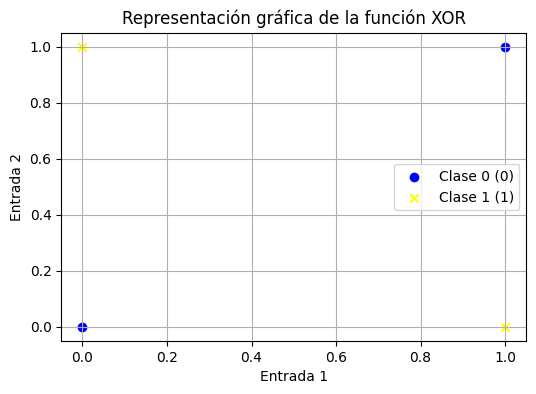
\includegraphics[width=0.5\textwidth]{imgs/XOR/XOR_grafica.png}
    \caption{XOR como un problema de clasificación no lineal}
    \label{fig:xor_plot}
\end{figure}

Para poder construir la red neuronal que resuelva el problema, vamos a utilizar las entradas del XOR como las muestras $\vec{x}\in \mathbb{R}^2$; y las salidas como el conjunto $T$ u objetivos (\textit{targets}).

\subsection{Arquitectura de la red XOR}

Para resolver el problema del XOR, se define una arquitectura de $D=2$ neuronas de entrada; $M=2$ neuronas en la capa oculta; y $K=1$ neuronas en la capa de salida. Esto se puede ver representado en la figura \ref{fig:xor_arqui}.

\begin{figure}[htbp]
    \centering
    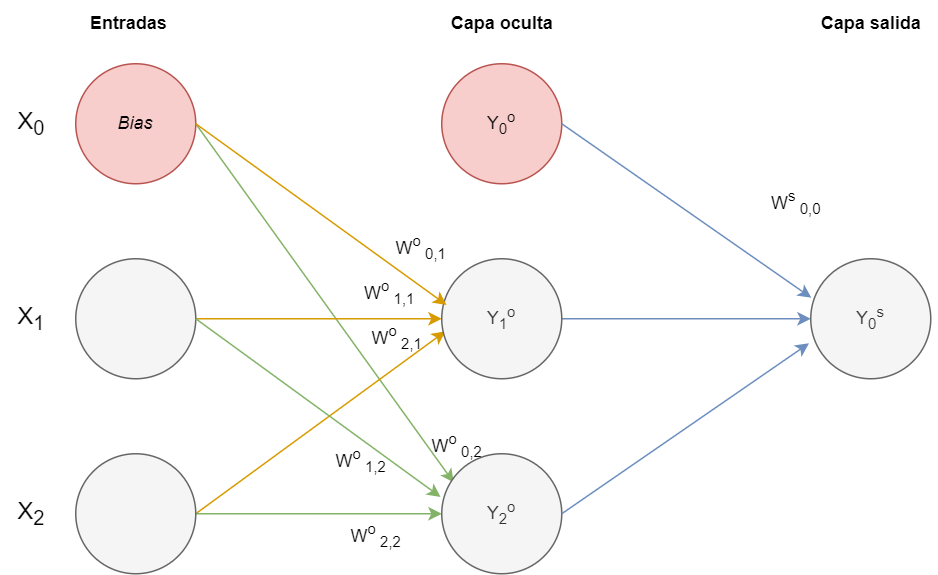
\includegraphics[width=0.5 \textwidth]{imgs/XOR/xor_arquitecture.png}
    \caption{Arquitectura de la red del XOR}
    \label{fig:xor_arqui}
\end{figure}

\subsection{Entrenamiento de la red  XOR y convergencia}

Se entrenó la red con distintas combinaciones de parámetros para encontrar cuáles producían la salida esperada. En el cuadro \ref{tab:xor_converge_table}, se documentan los parámetros para los cuales la red tuvo una convergencia, es decir, se alcanzó un error de $0$ (o al menos cercano a 0).

\begin{table}[!ht]
\centering
\begin{tabular}{c|c|c|c}
\hline
\textbf{Configuración} & \textbf{$\alpha$} & \textbf{$\gamma$} & \textbf{Épocas} \\
\hline
1 & 0.05 & 0.7 & 150 \\
2 & 0.05 & 0.9 & 75 \\
3 & 0.1 & 0.0001 & 200 \\
4 & 0.1 & 0.3 & 150 \\
5 & 0.1 & 0.08 & 200 \\
6 & 0.1 & 0.7 & 50 \\
7 & 0.1 & 0.9 & 50 \\
\hline
\end{tabular}
\caption{Hiperparámetros probados para la red neuronal del XOR que presentaron convergencia}
\label{tab:xor_converge_table}
\end{table}

Para la configuración 1: $\alpha=0.05, \gamma=0.7$; con $150$ épocas, se tiene que la red converge alcanzadas las $90$ épocas de entrenamiento, tal y como se muestra en la figura \ref{fig:conf1_lr_con_xor}.

% config 1 XOR
\begin{figure}[h!]
    \centering
    \begin{subfigure}{0.49\textwidth}
        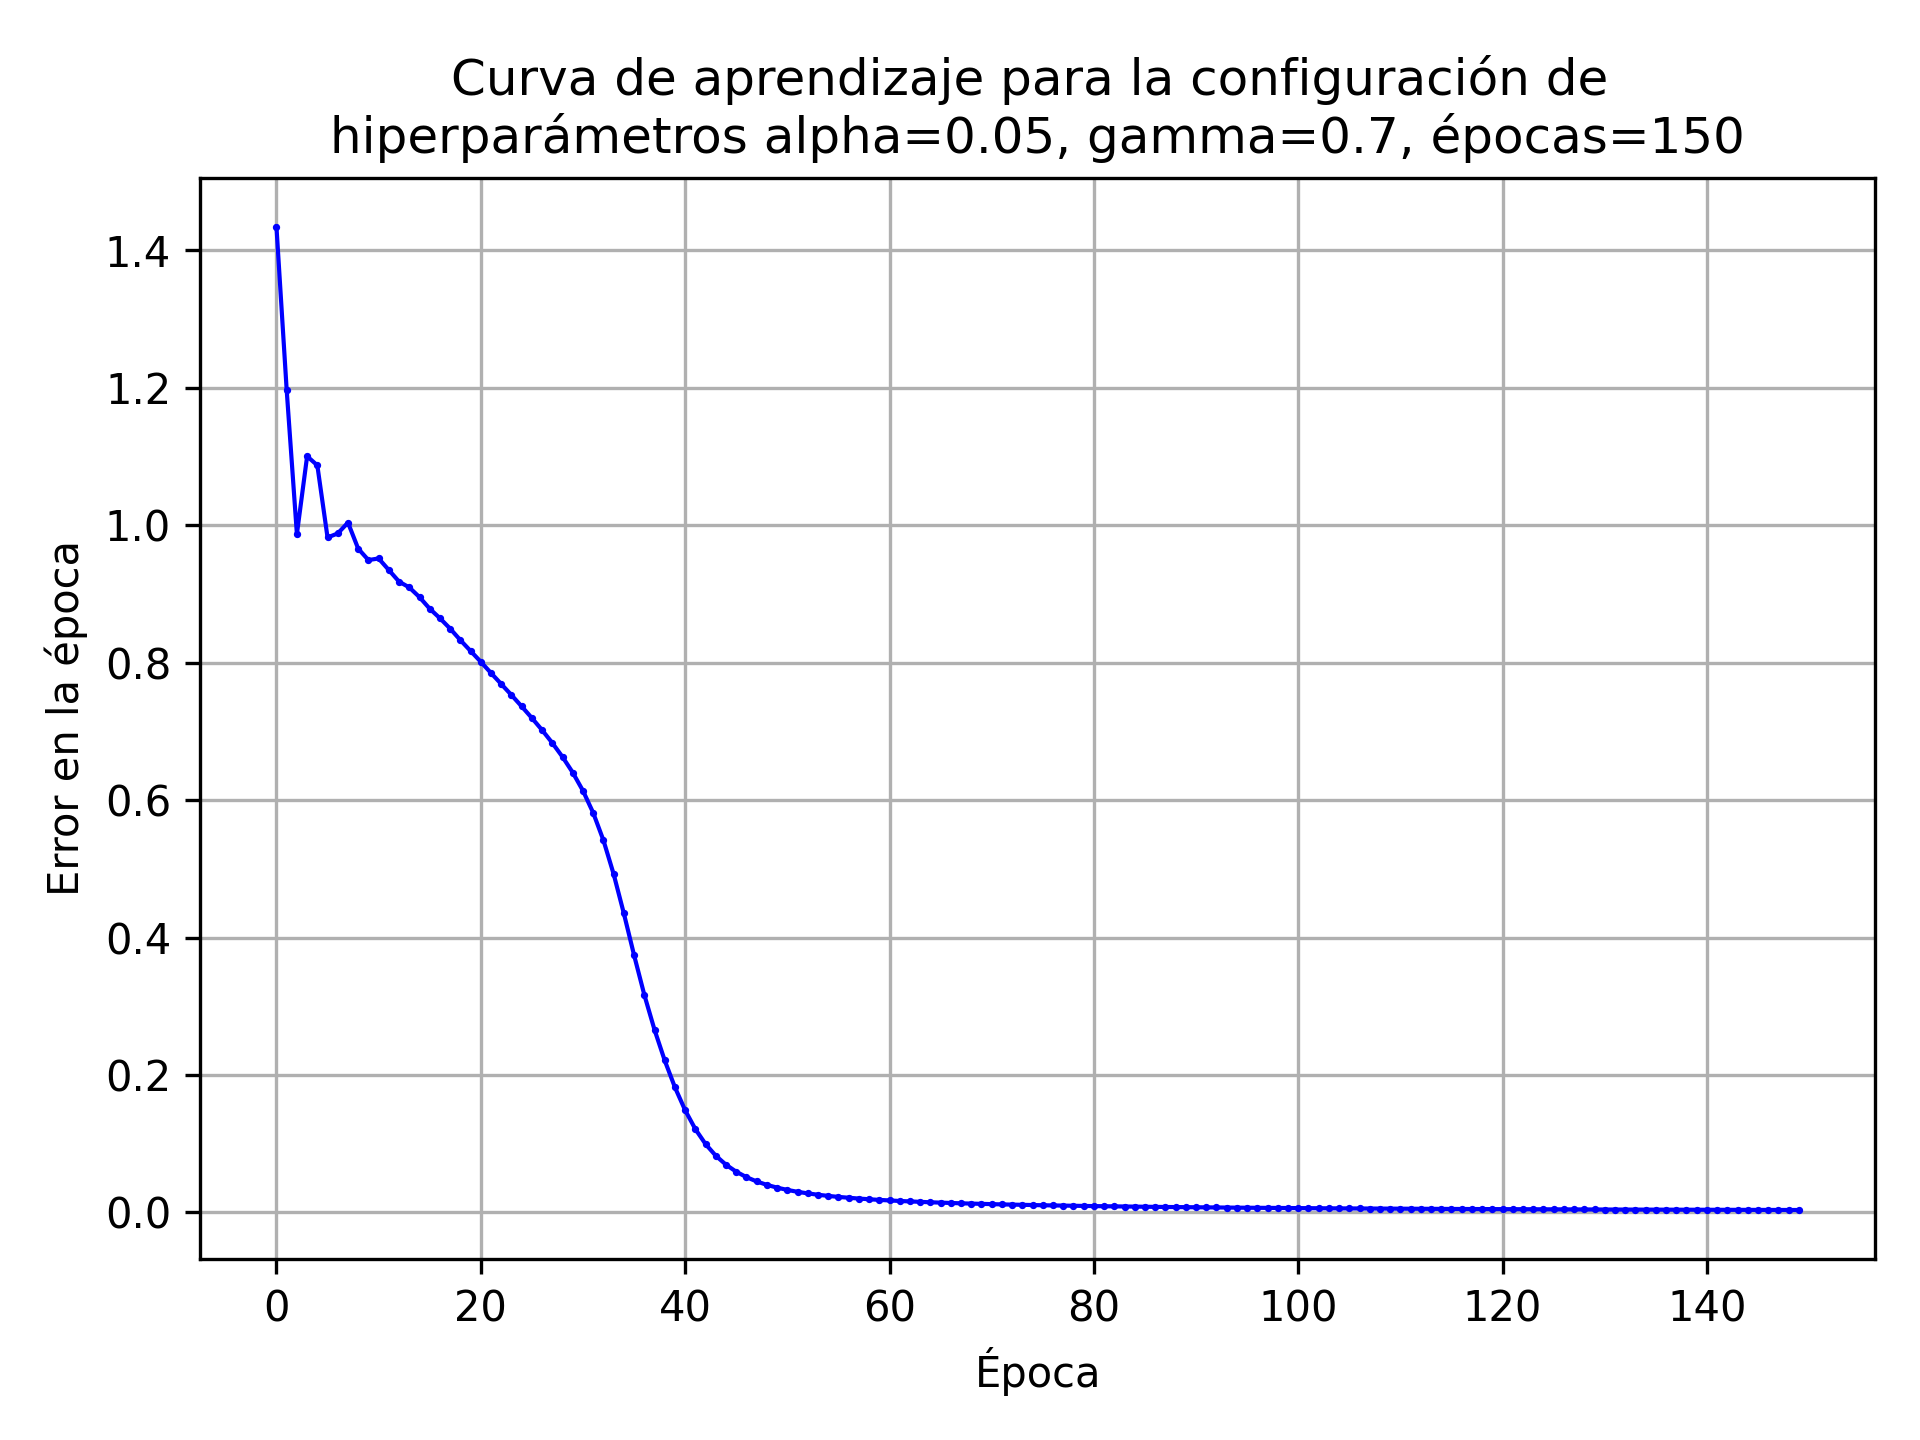
\includegraphics[width=\textwidth]{imgs/XOR/configs/curva_aprendizaje_alpha_0.05_gamma_0.7_epochs_150.png}
        \caption{Curva de aprendizaje de la configuración 1}
        \label{fig:conf_1_xor_lr}
    \end{subfigure}
    \hfill
    \begin{subfigure}{0.49\textwidth}
        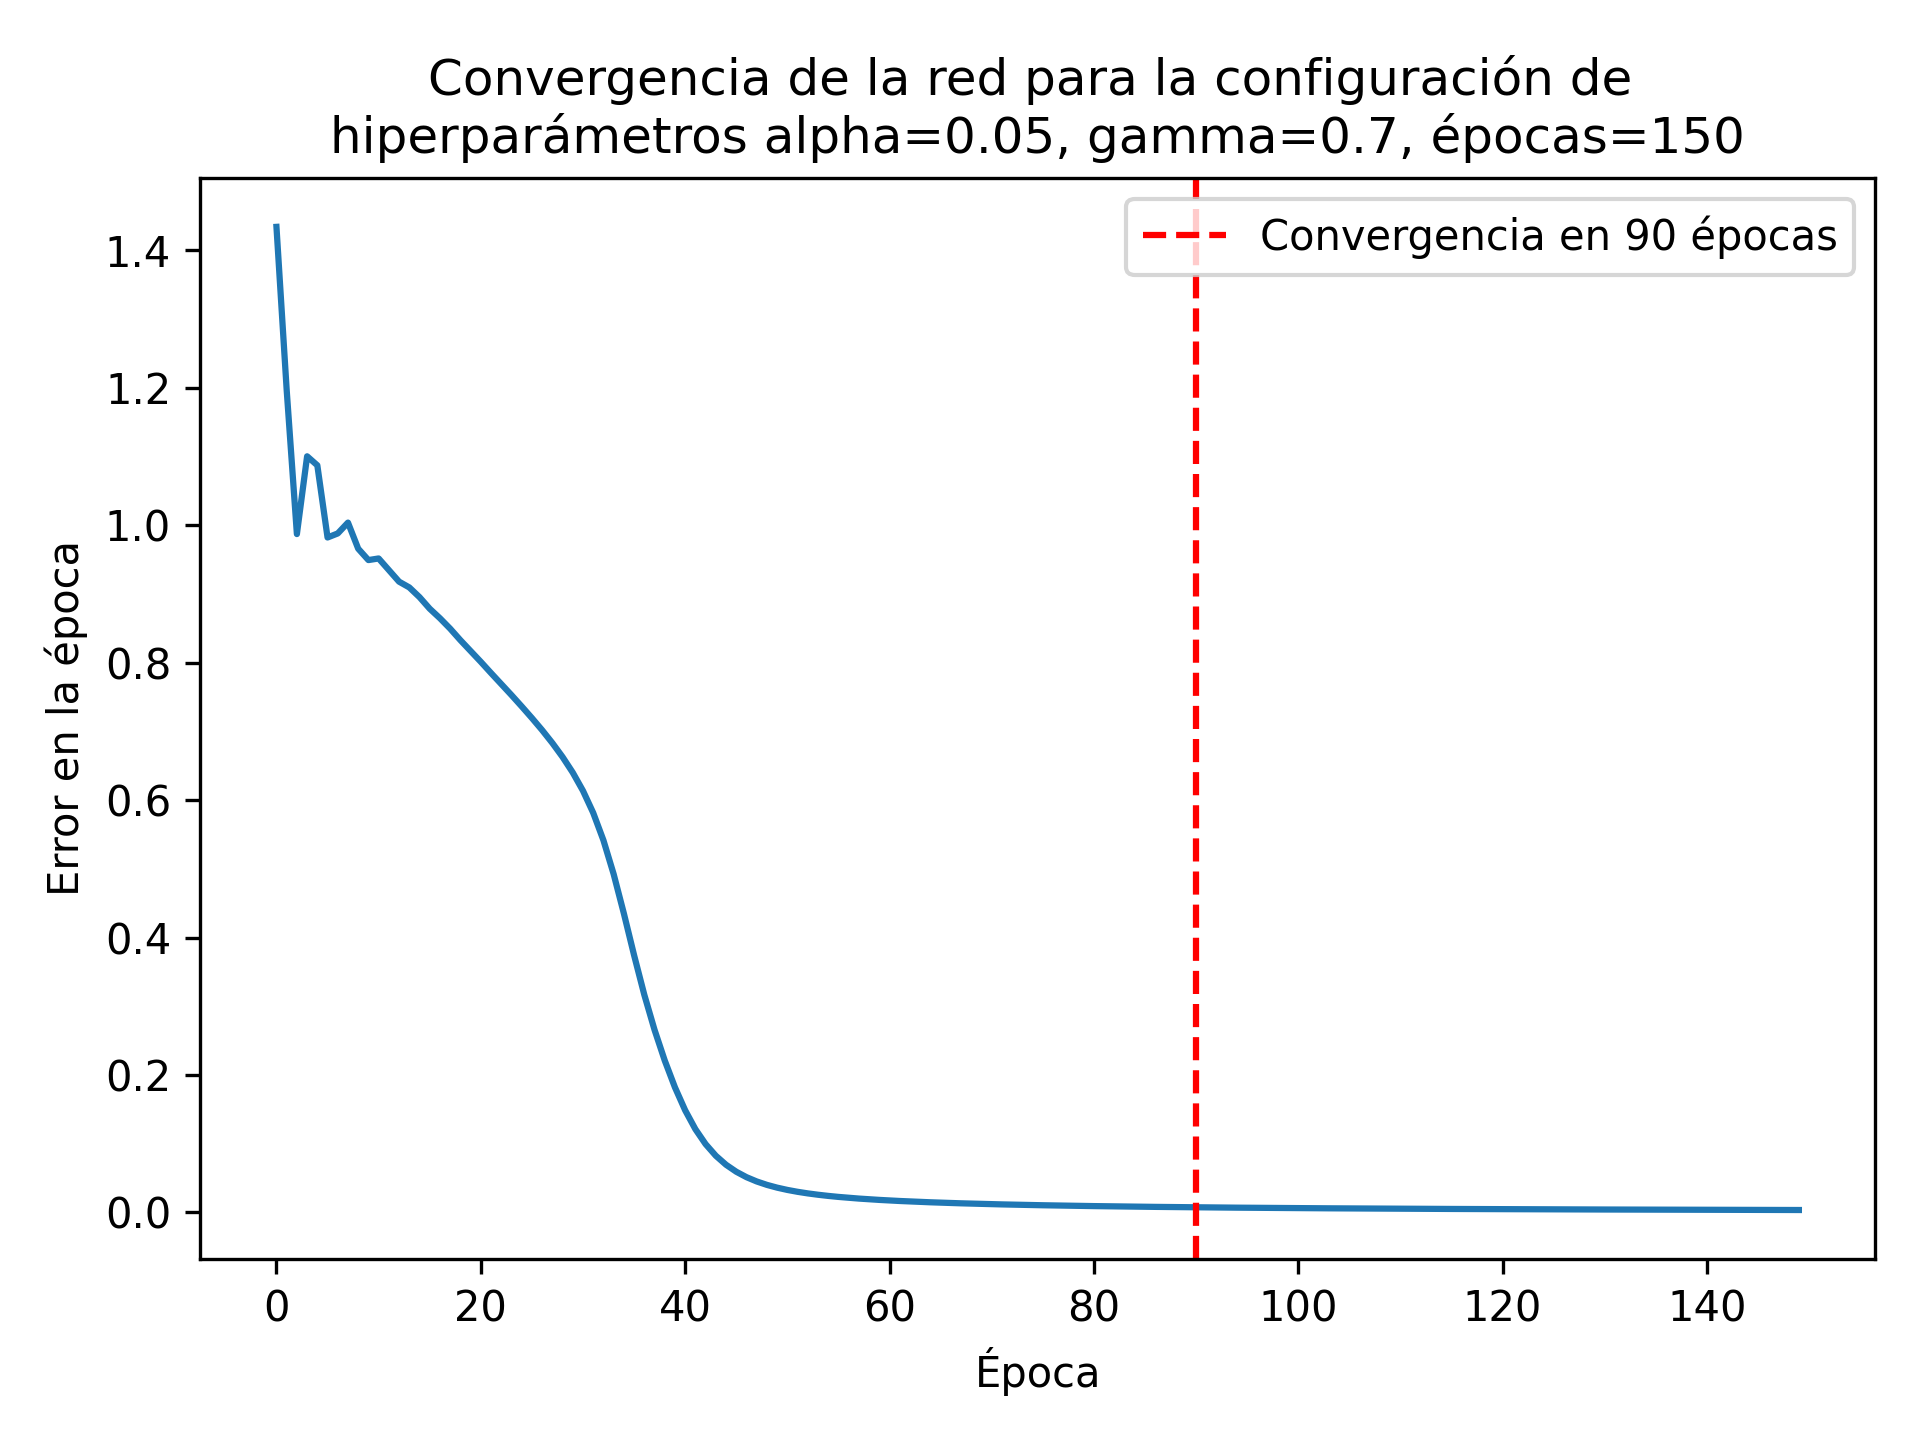
\includegraphics[width=\textwidth]{imgs/XOR/configs/convergencia_alpha_0.05_gamma_0.7_epochs_150.png}
        \caption{Convergencia de la configuración 1}
        \label{fig:conf1_xor_con}
    \end{subfigure}
    \caption{Curva de aprendizaje y convergencia para la configuración 1}
    \label{fig:conf1_lr_con_xor}
\end{figure}

Para la configuración 2: $\alpha=0.05, \gamma=0.9$; con $75$ épocas, la red converge alcanzadas las $40$ épocas. Si vemos la figura \ref{fig:conf2_lr_con_xor}, se puede deducir que al modificar el hiperparámetro $\gamma$ y colocar uno más grande, la red converge en una menor cantidad de épocas para el mismo valor de $\alpha$. 

\newpage
% Config 2 XOR
\begin{figure}[h!]
    \centering
    \begin{subfigure}{0.49\textwidth}
        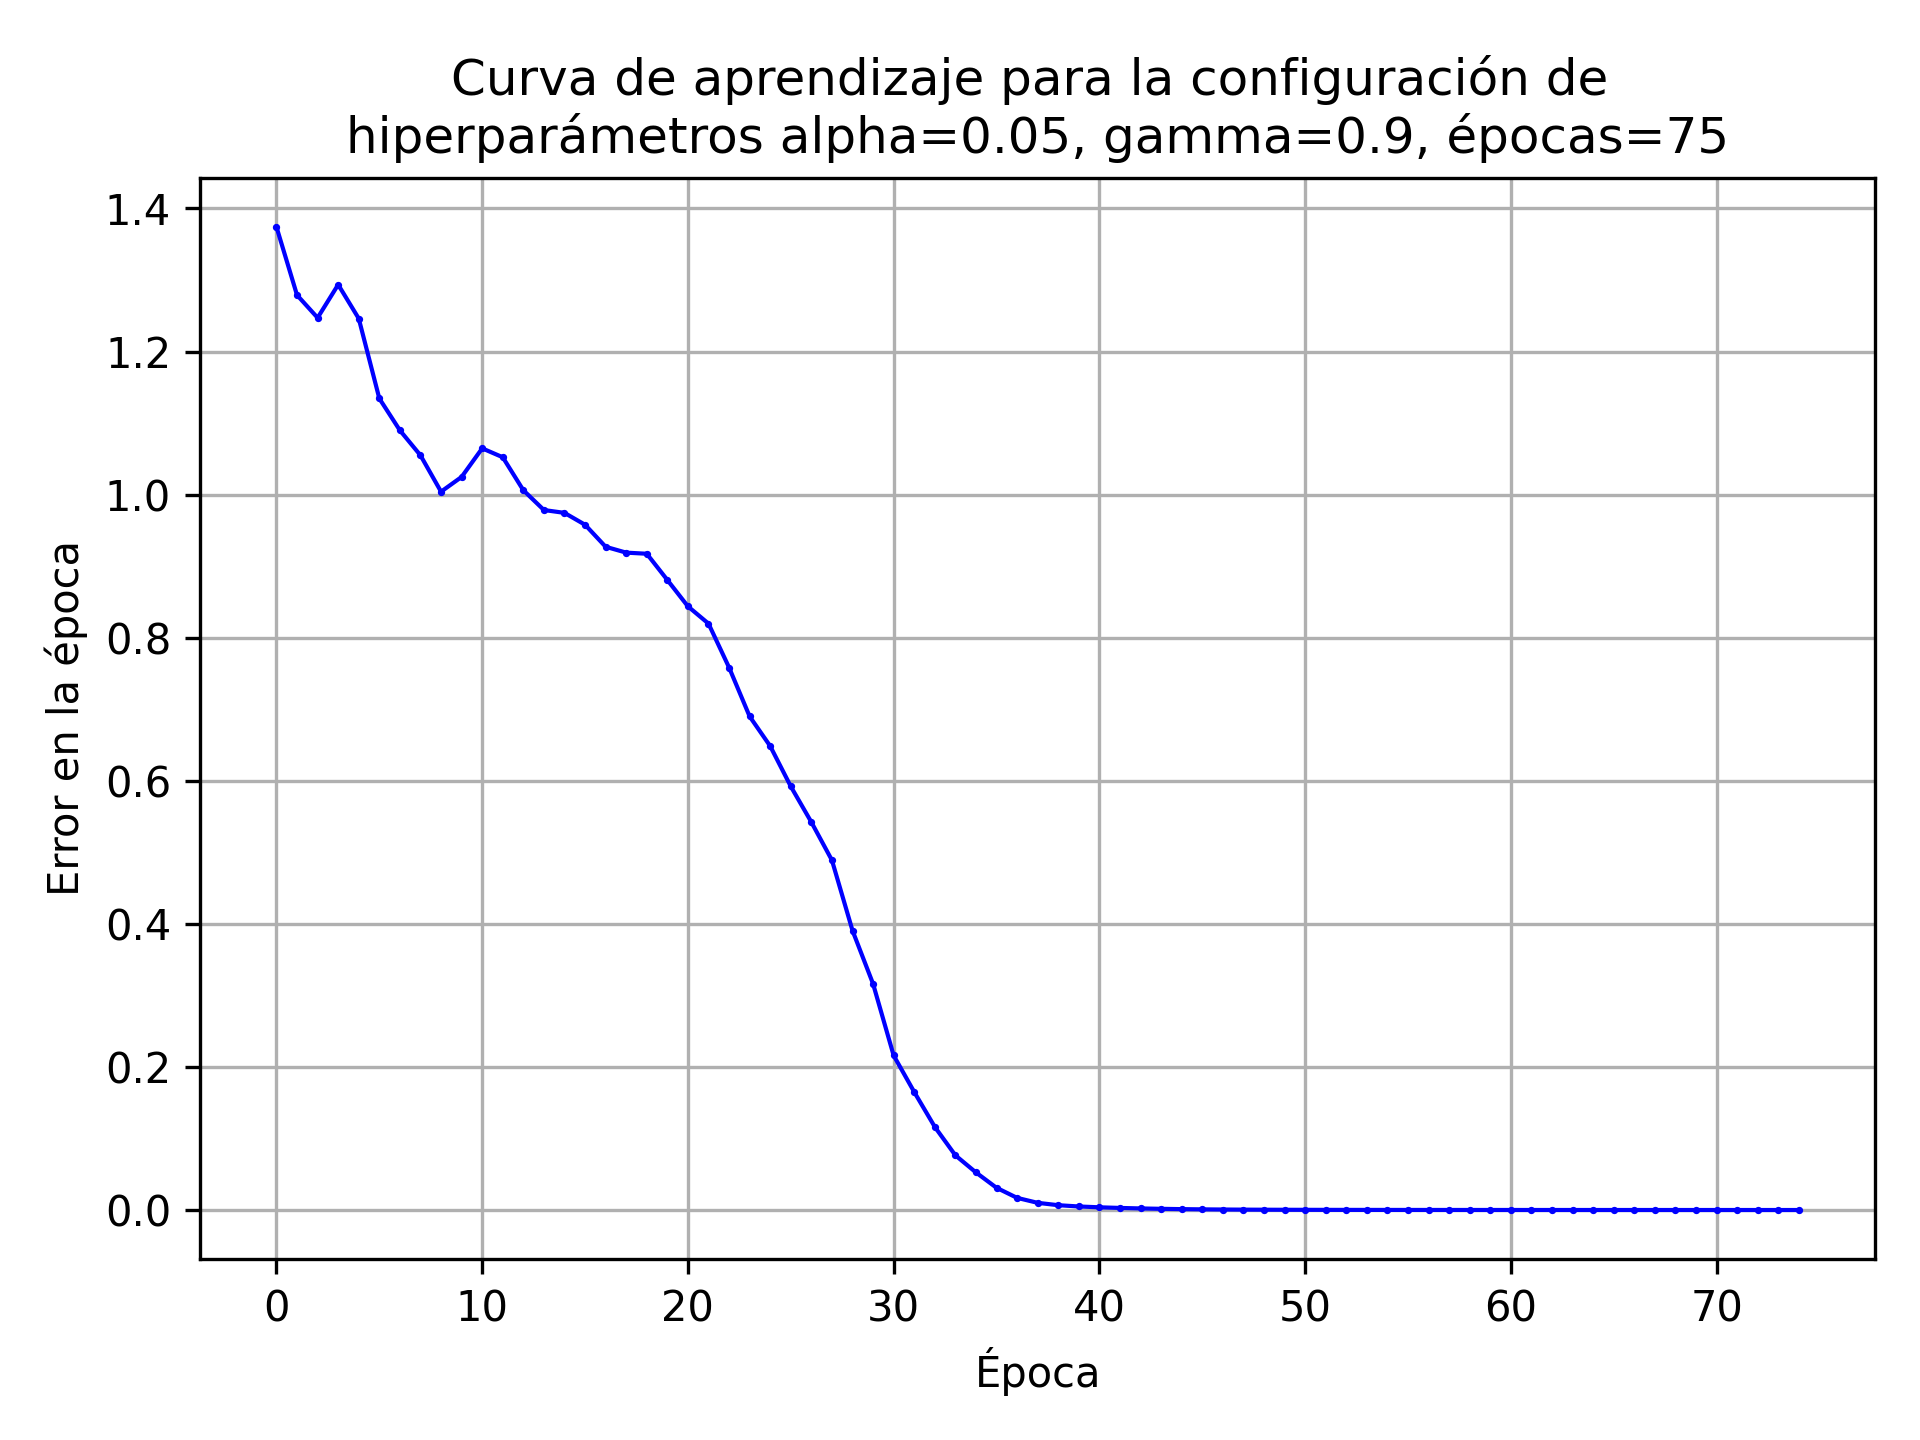
\includegraphics[width=\textwidth]{imgs/XOR/configs/curva_aprendizaje_alpha_0.05_gamma_0.9_epochs_75.png}
        \caption{Curva de aprendizaje de la configuración 2}
        \label{fig:conf_2_xor_lr}
    \end{subfigure}
    \hfill
    \begin{subfigure}{0.49\textwidth}
        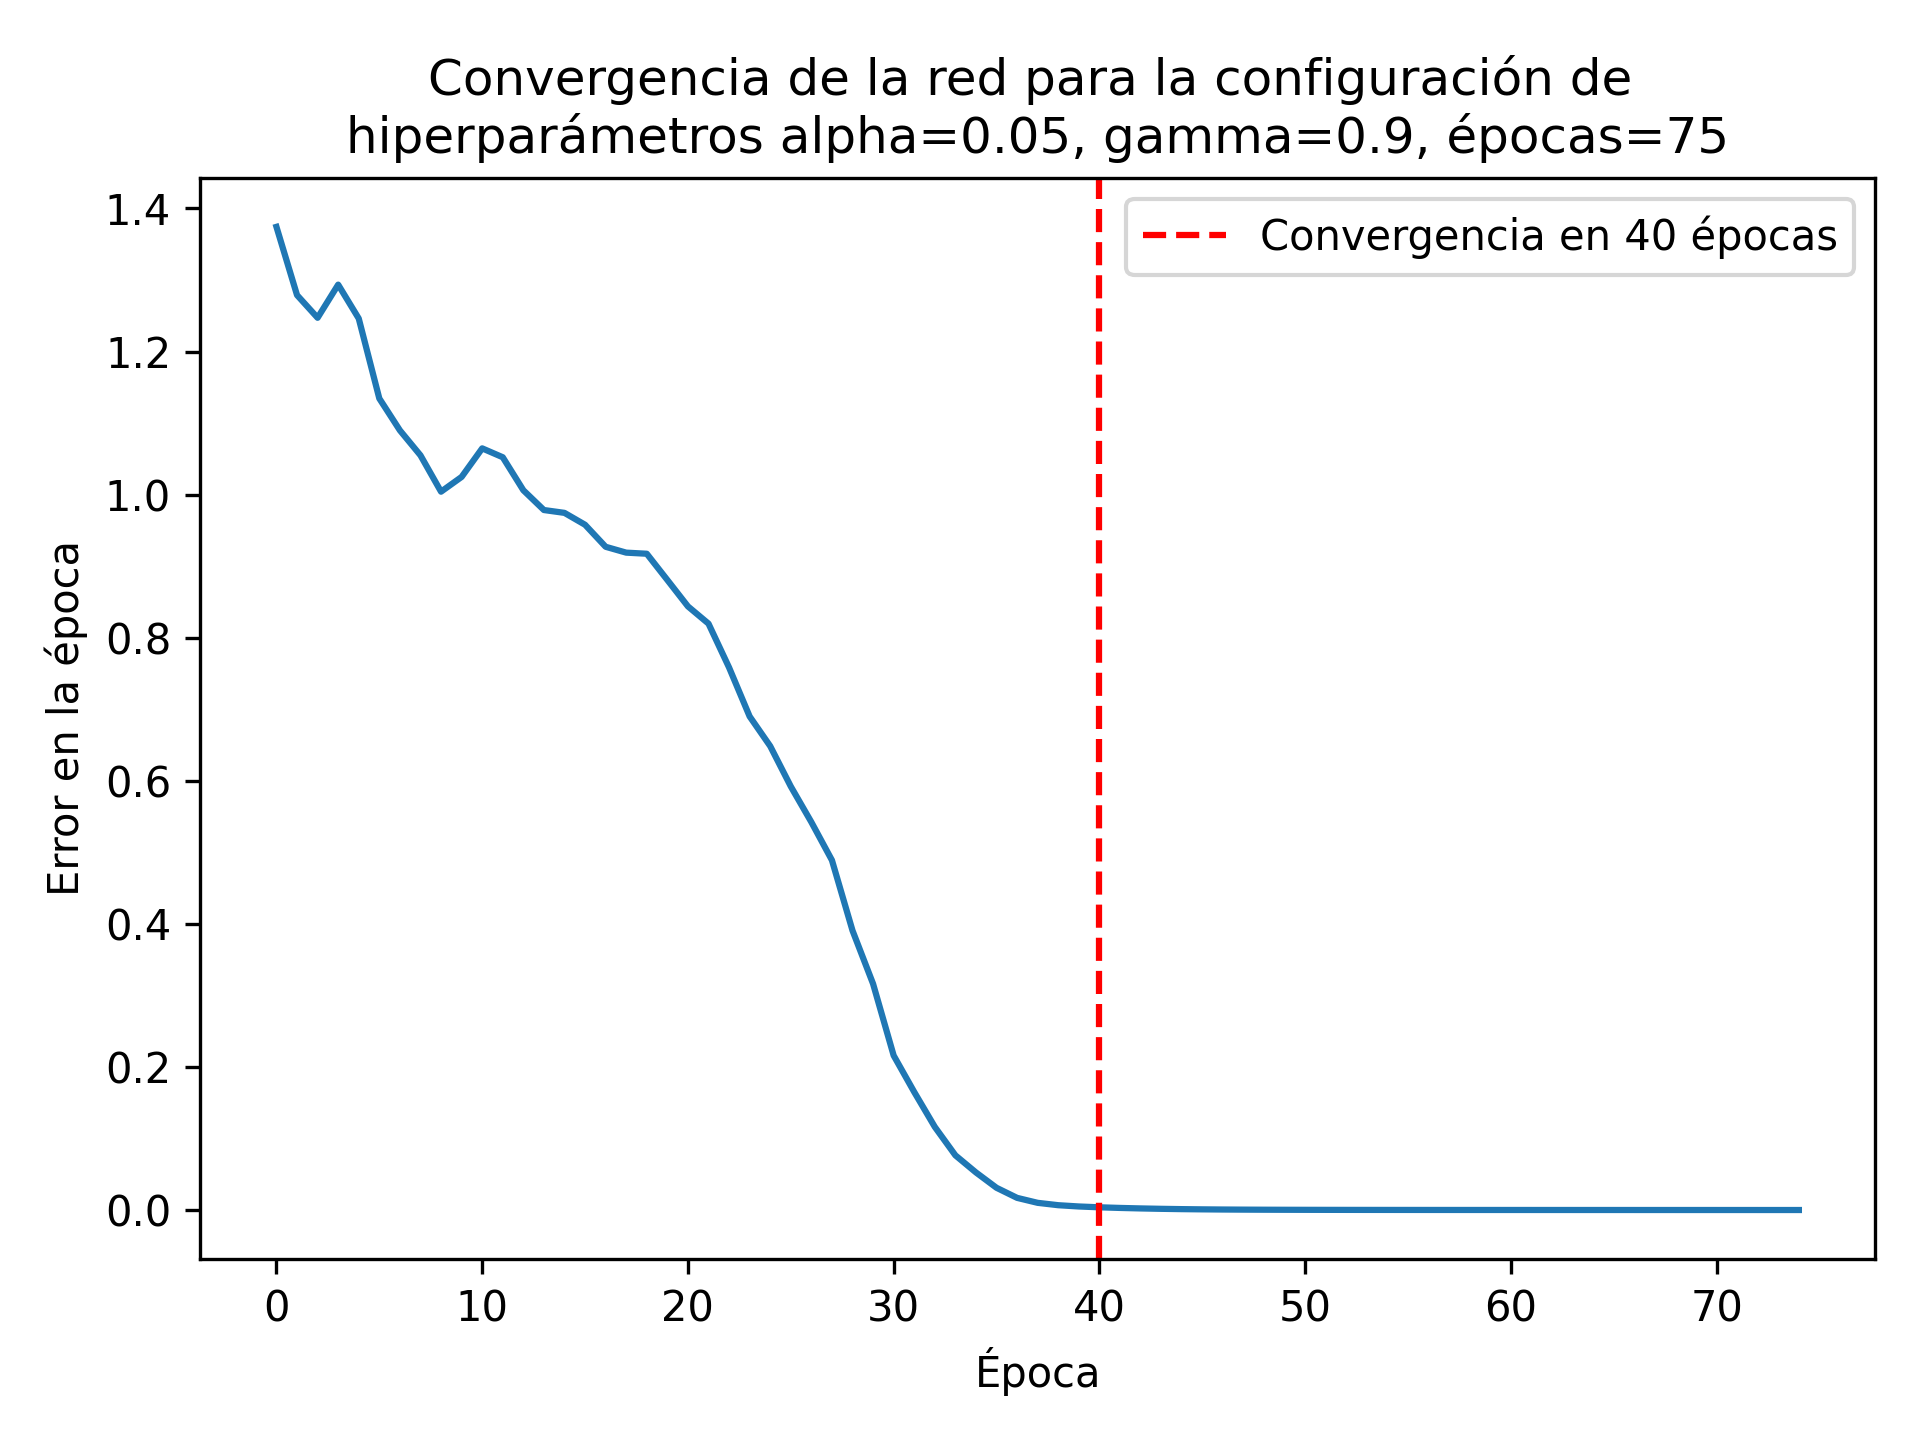
\includegraphics[width=\textwidth]{imgs/XOR/configs/convergencia_alpha_0.05_gamma_0.9_epochs_75.png}
        \caption{Convergencia de la configuración 2}
        \label{fig:conf2_xor_con}
    \end{subfigure}
    \caption{Curva de aprendizaje y convergencia para la configuración 2}
    \label{fig:conf2_lr_con_xor}
\end{figure}

Ahora bien, para la configuración 3: $\alpha=0.1, \gamma=0.0001$; con $200$ épocas, se puede observar que con un $\alpha$ un poco más grande, la red de igual forma converge aún si el parámetro $\gamma$ es muy cercano a $0$. Esto se puede apreciar en la figura \ref{fig:conf3_lr_con_xor}. 

% Config 3 XOR
\begin{figure}[h!]
    \centering
    \begin{subfigure}{0.49\textwidth}
        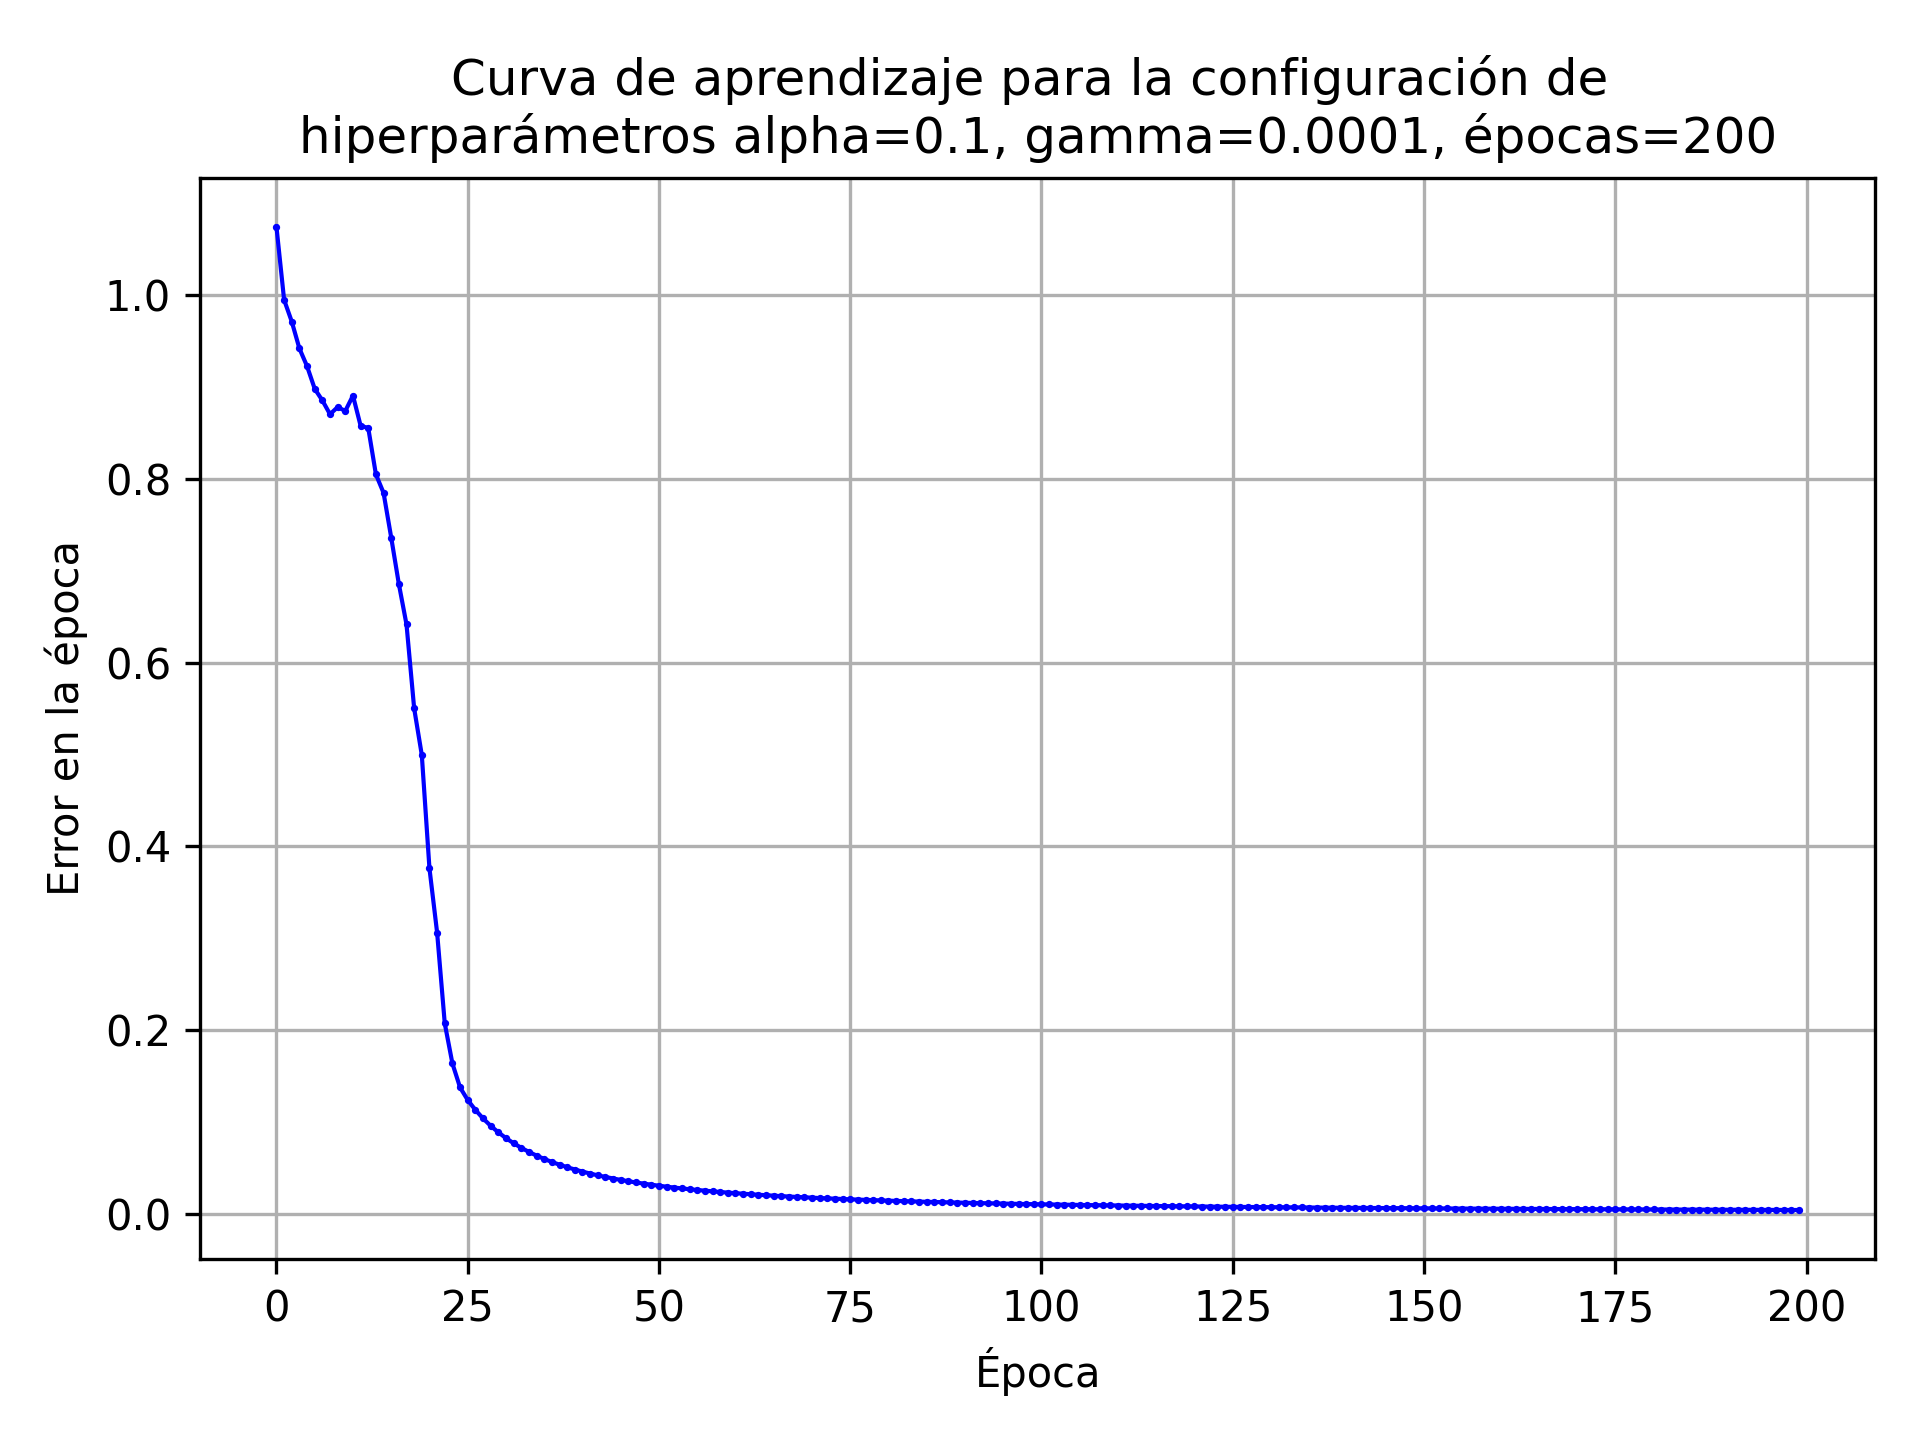
\includegraphics[width=\textwidth]{imgs/XOR/configs/curva_aprendizaje_alpha_0.1_gamma_0.0001_epochs_200.png}
        \caption{Curva de aprendizaje de la configuración 3}
        \label{fig:conf_3_xor_lr}
    \end{subfigure}
    \hfill
    \begin{subfigure}{0.49\textwidth}
        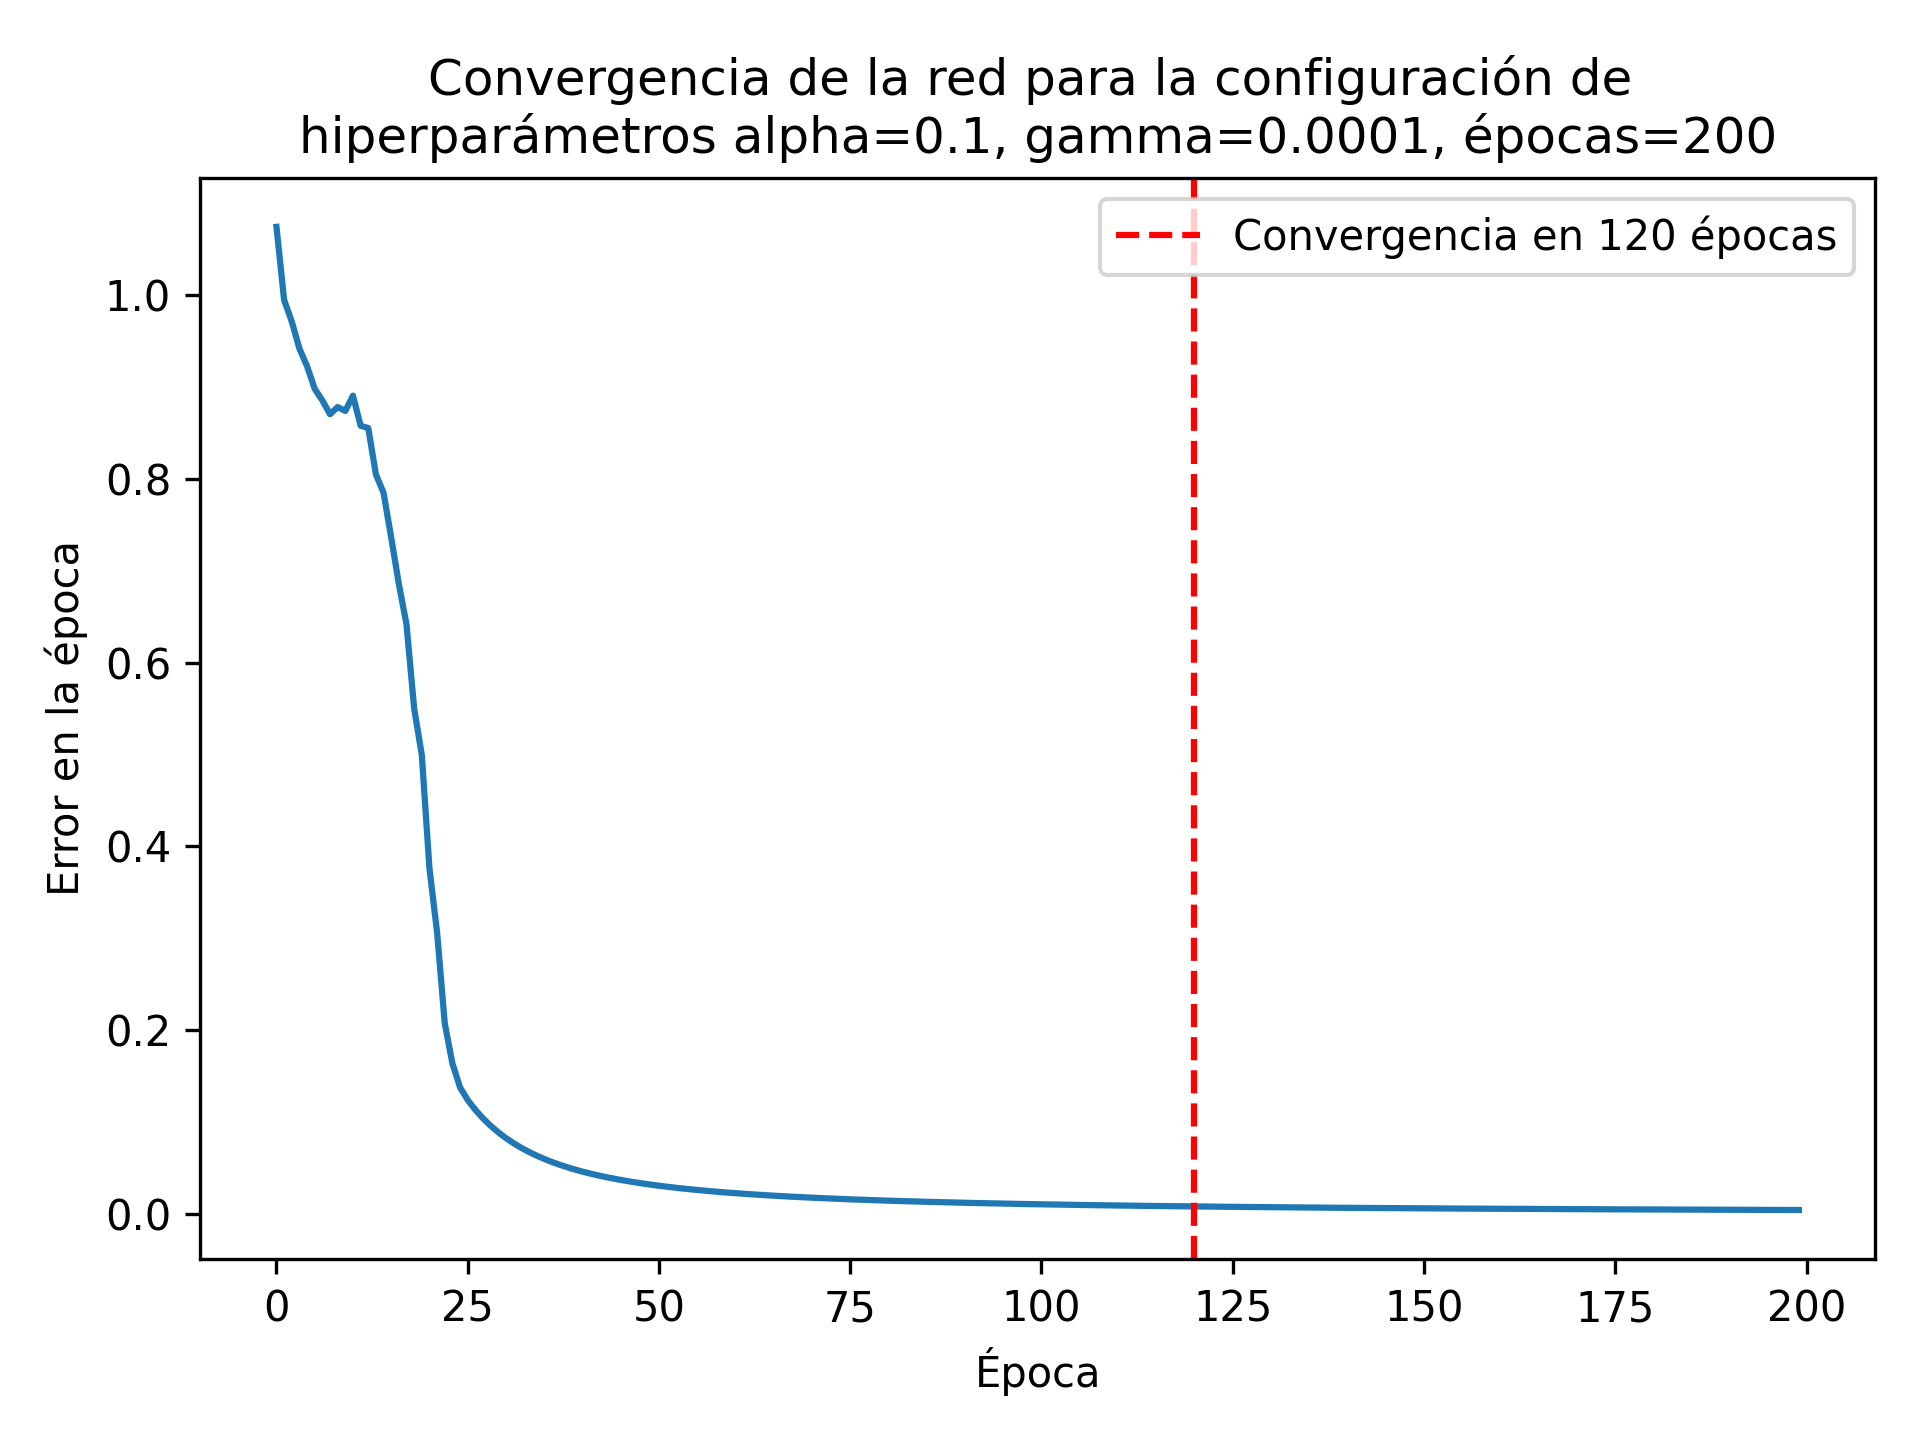
\includegraphics[width=\textwidth]{imgs/XOR/configs/convergencia_alpha_0.1_gamma_0.0001_epochs_200.png}
        \caption{Convergencia de la configuración 3}
        \label{fig:conf3_xor_con}
    \end{subfigure}
    \caption{Curva de aprendizaje y convergencia para la configuración 3}
    \label{fig:conf3_lr_con_xor}
\end{figure}

Con la configuración 4: $\alpha=0.1, \gamma=0.3$; y épocas igual a 150, se puede observar en la figura \ref{fig:conf4_lr_con_xor} que, pareciera que el hiperparámetro $\gamma$ no tiene influencia significativa cuando el valor $\alpha$ es igual a $0.1$, esto debido a que no se presenta una diferencia importante con lo presentado en la figura \ref{fig:conf3_lr_con_xor}.

% Config 4 XOR
\begin{figure}[h!]
    \centering
    \begin{subfigure}{0.49\textwidth}
        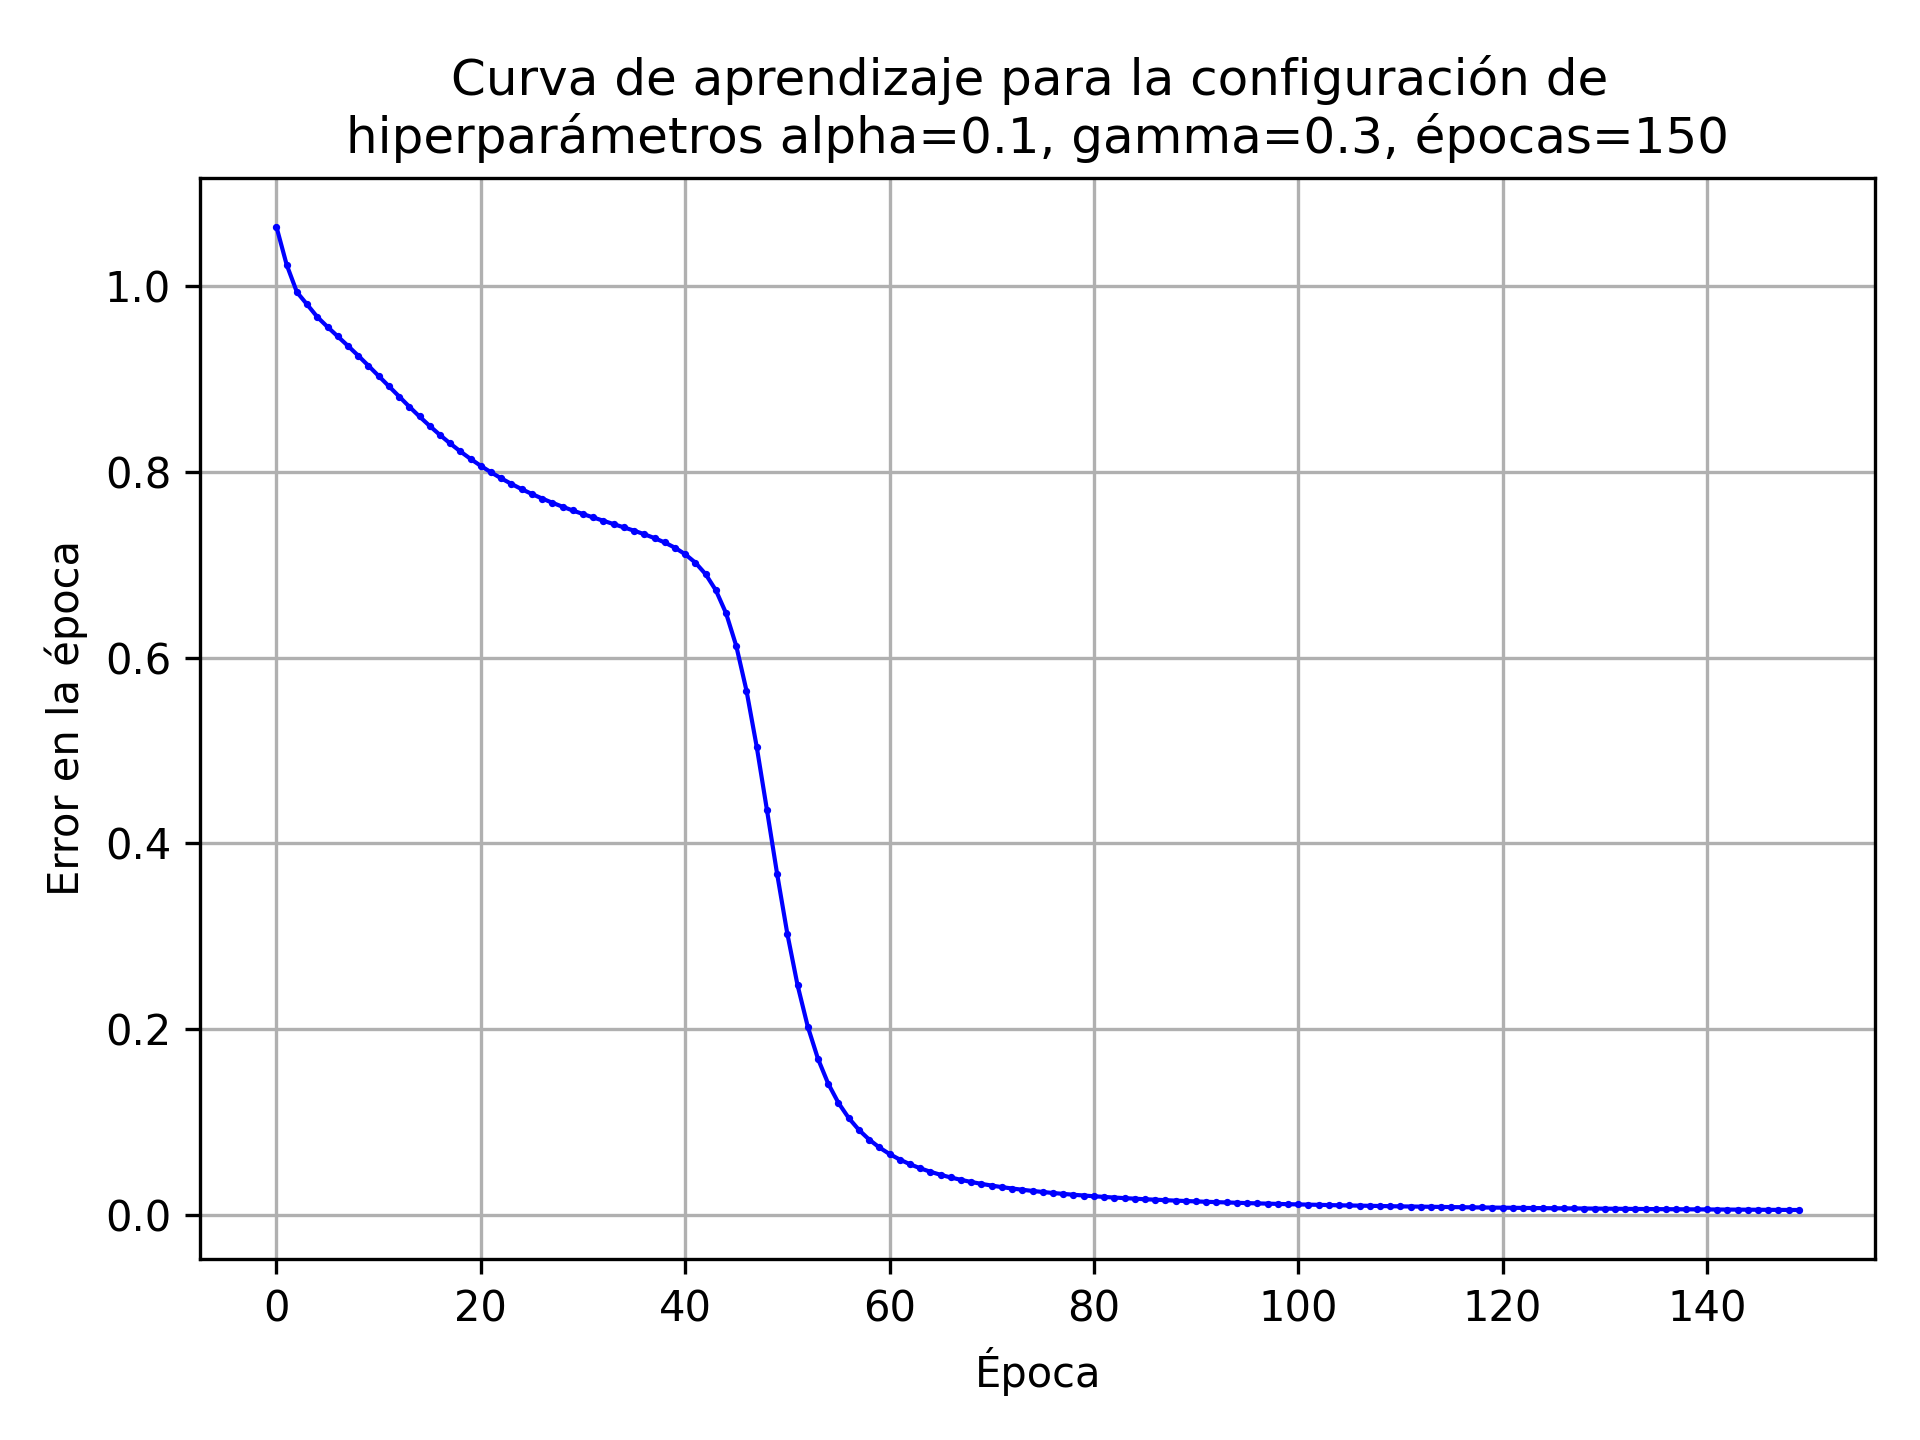
\includegraphics[width=\textwidth]{imgs/XOR/configs/curva_aprendizaje_alpha_0.1_gamma_0.3_epochs_150.png}
        \caption{Curva de aprendizaje de la configuración 4}
        \label{fig:conf_4_xor_lr}
    \end{subfigure}
    \hfill
    \begin{subfigure}{0.49\textwidth}
        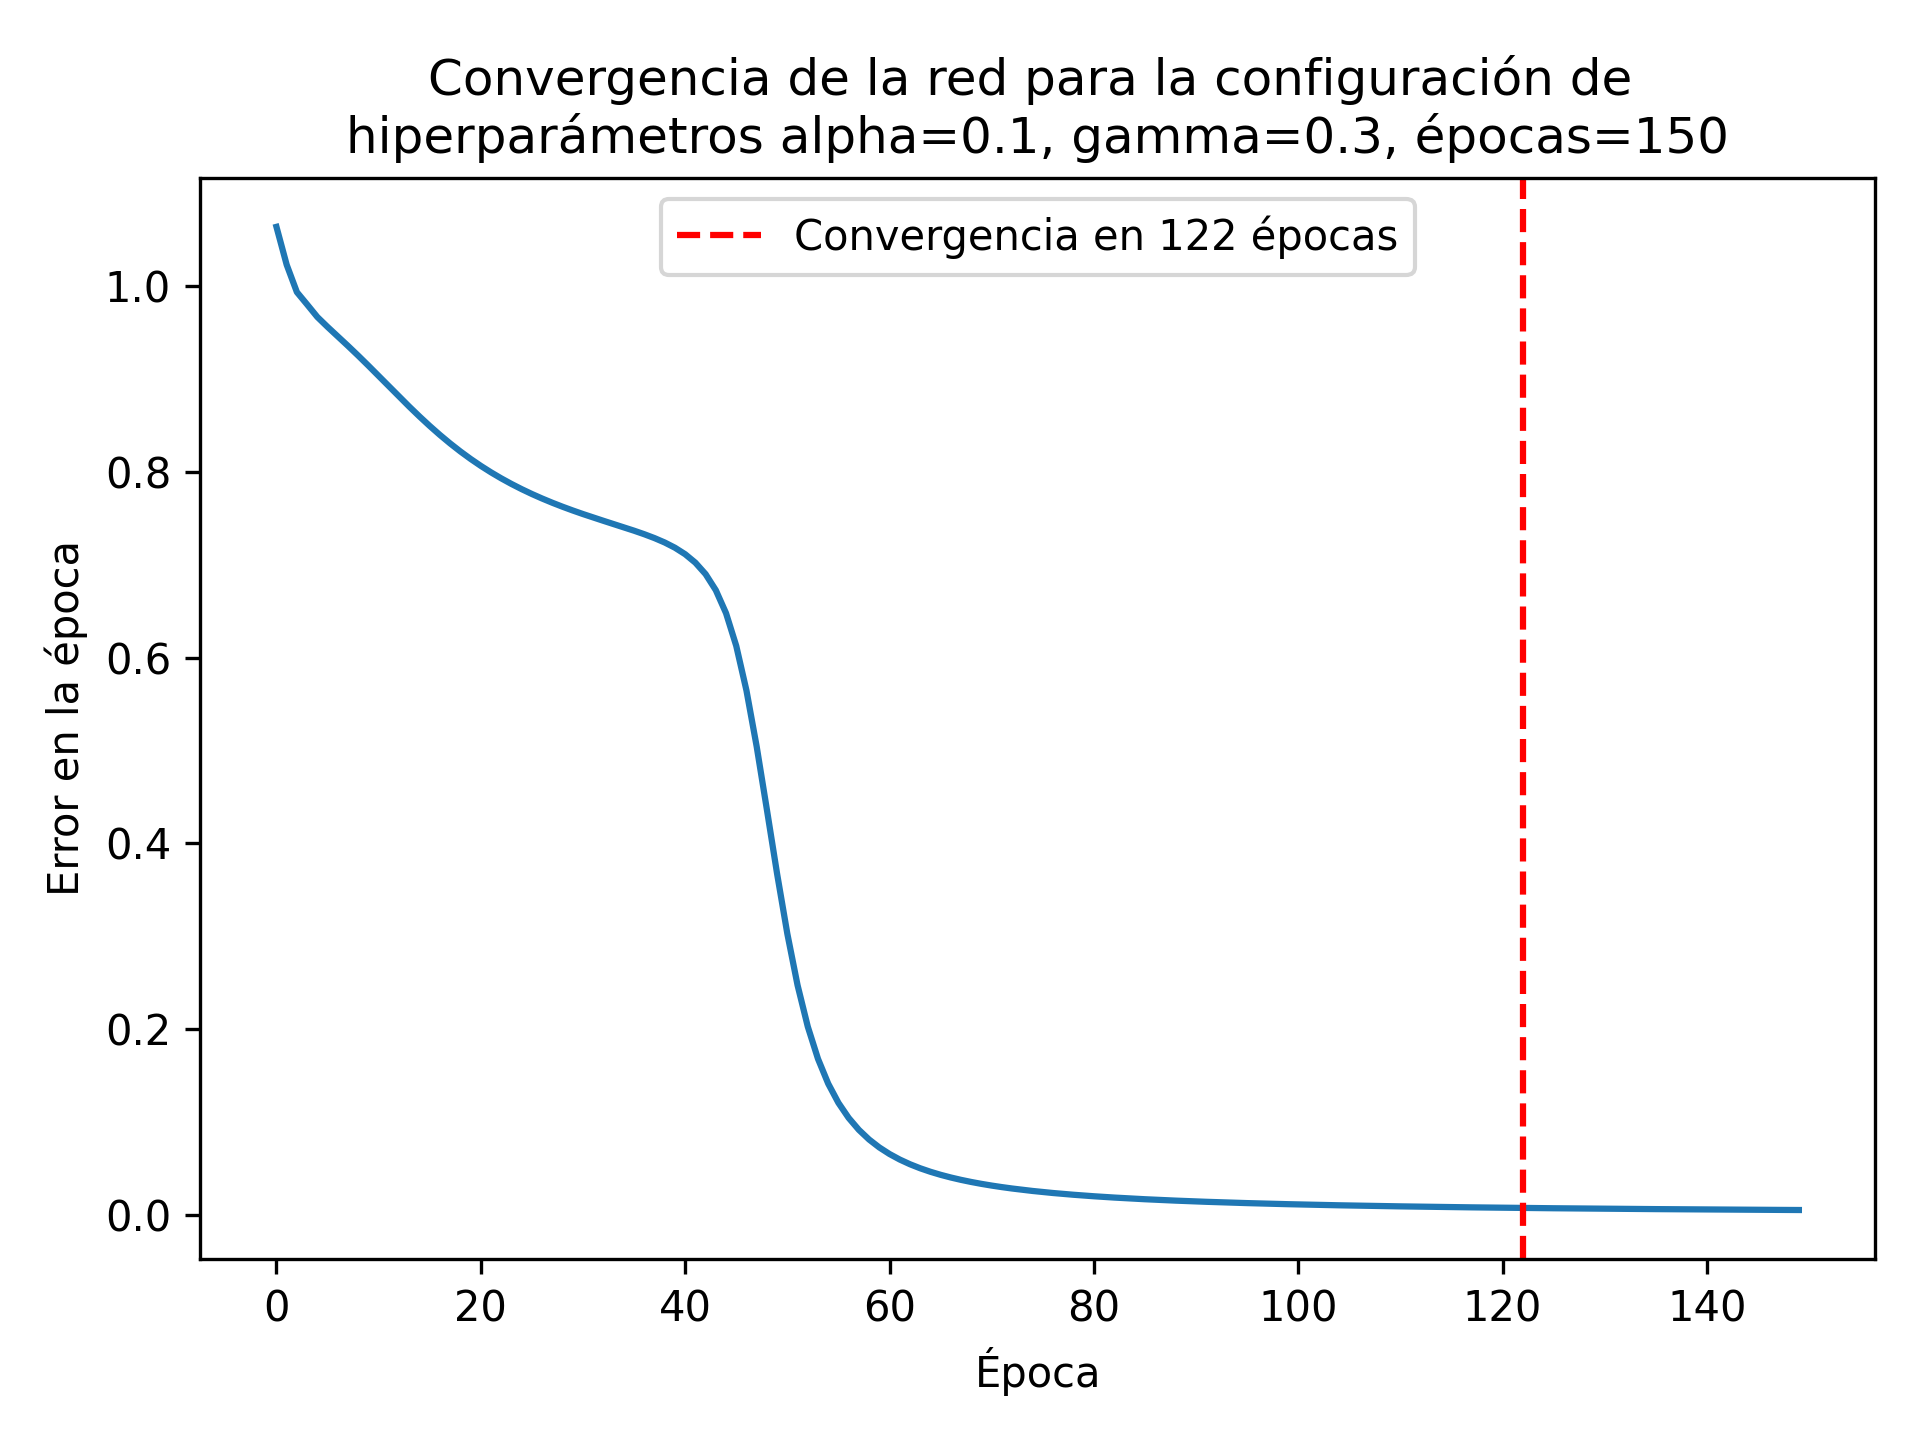
\includegraphics[width=\textwidth]{imgs/XOR/configs/convergencia_alpha_0.1_gamma_0.3_epochs_150.png}
        \caption{Convergencia de la configuración 4}
        \label{fig:conf4_xor_con}
    \end{subfigure}
    \caption{Curva de aprendizaje y convergencia para la configuración 4}
    \label{fig:conf4_lr_con_xor}
\end{figure}
\newpage

No obstante, como podemos observar en las figuras  \ref{fig:conf5_lr_con_xor}, \ref{fig:conf6_lr_con_xor} y \ref{fig:conf7_lr_con_xor}; para las configuraciones 5, 6 y 7; se determina que, para un $\alpha=0.1$, el presentar un $\gamma$ más alto, hace que la red converja en una menor cantidad de épocas, más aún con un $\gamma=0.9$, como se presenta en la figura \ref{fig:conf7_lr_con_xor}.
% Config 5 XOR
\begin{figure}[h!]
    \centering
    \begin{subfigure}{0.49\textwidth}
        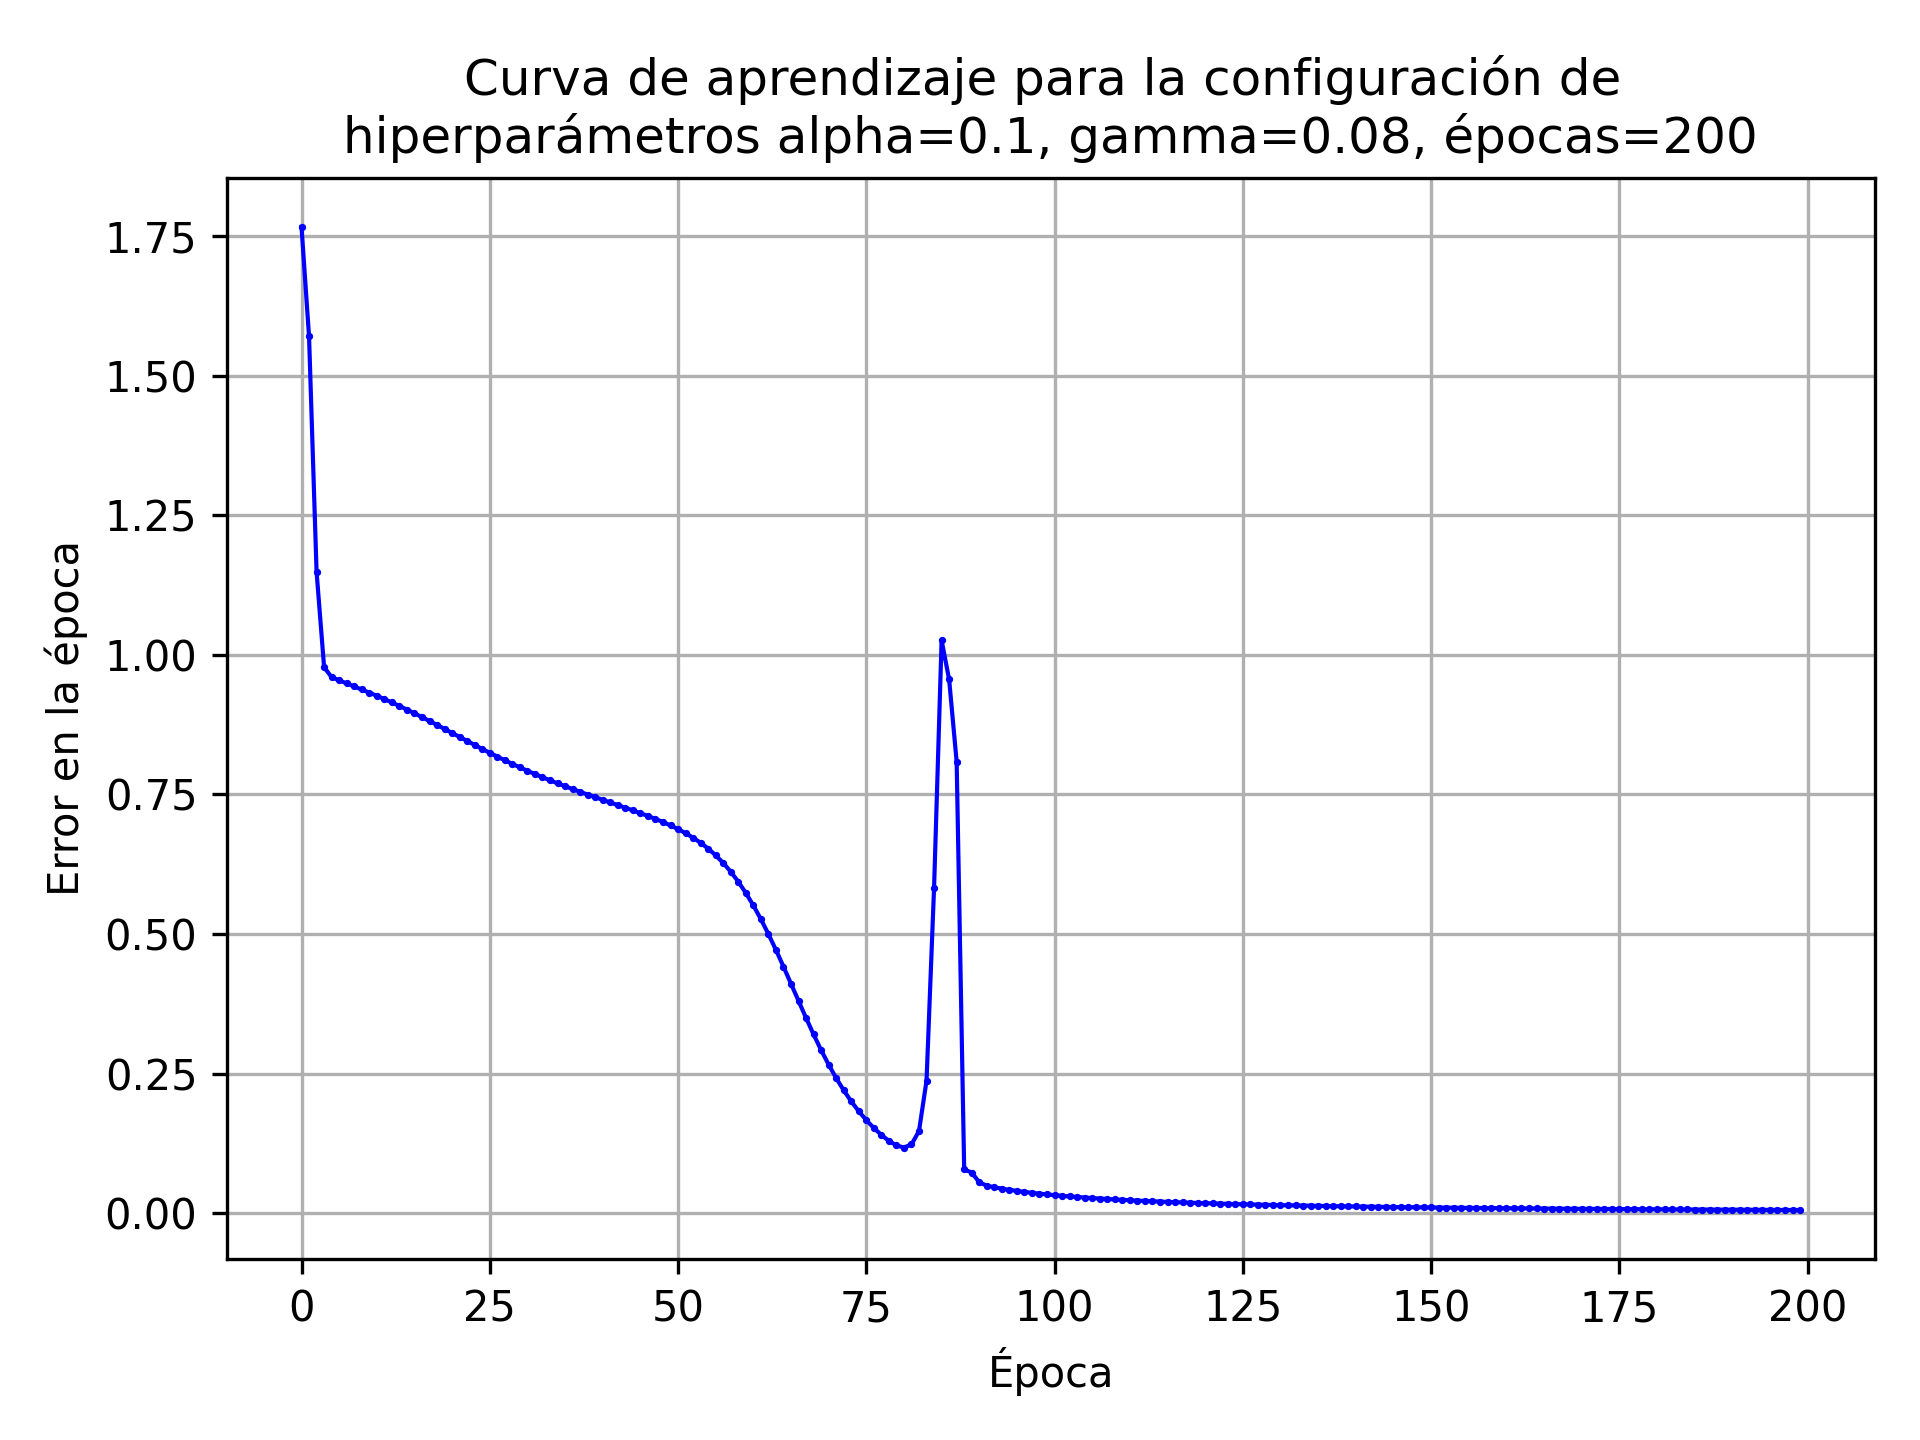
\includegraphics[width= \textwidth]{imgs/XOR/configs/curva_aprendizaje_alpha_0.1_gamma_0.08_epochs_200.png}
        \caption{Curva de aprendizaje de la configuración 5}
        \label{fig:conf_5_xor_lr}
    \end{subfigure}
    \hfill
    \begin{subfigure}{0.49\textwidth}
        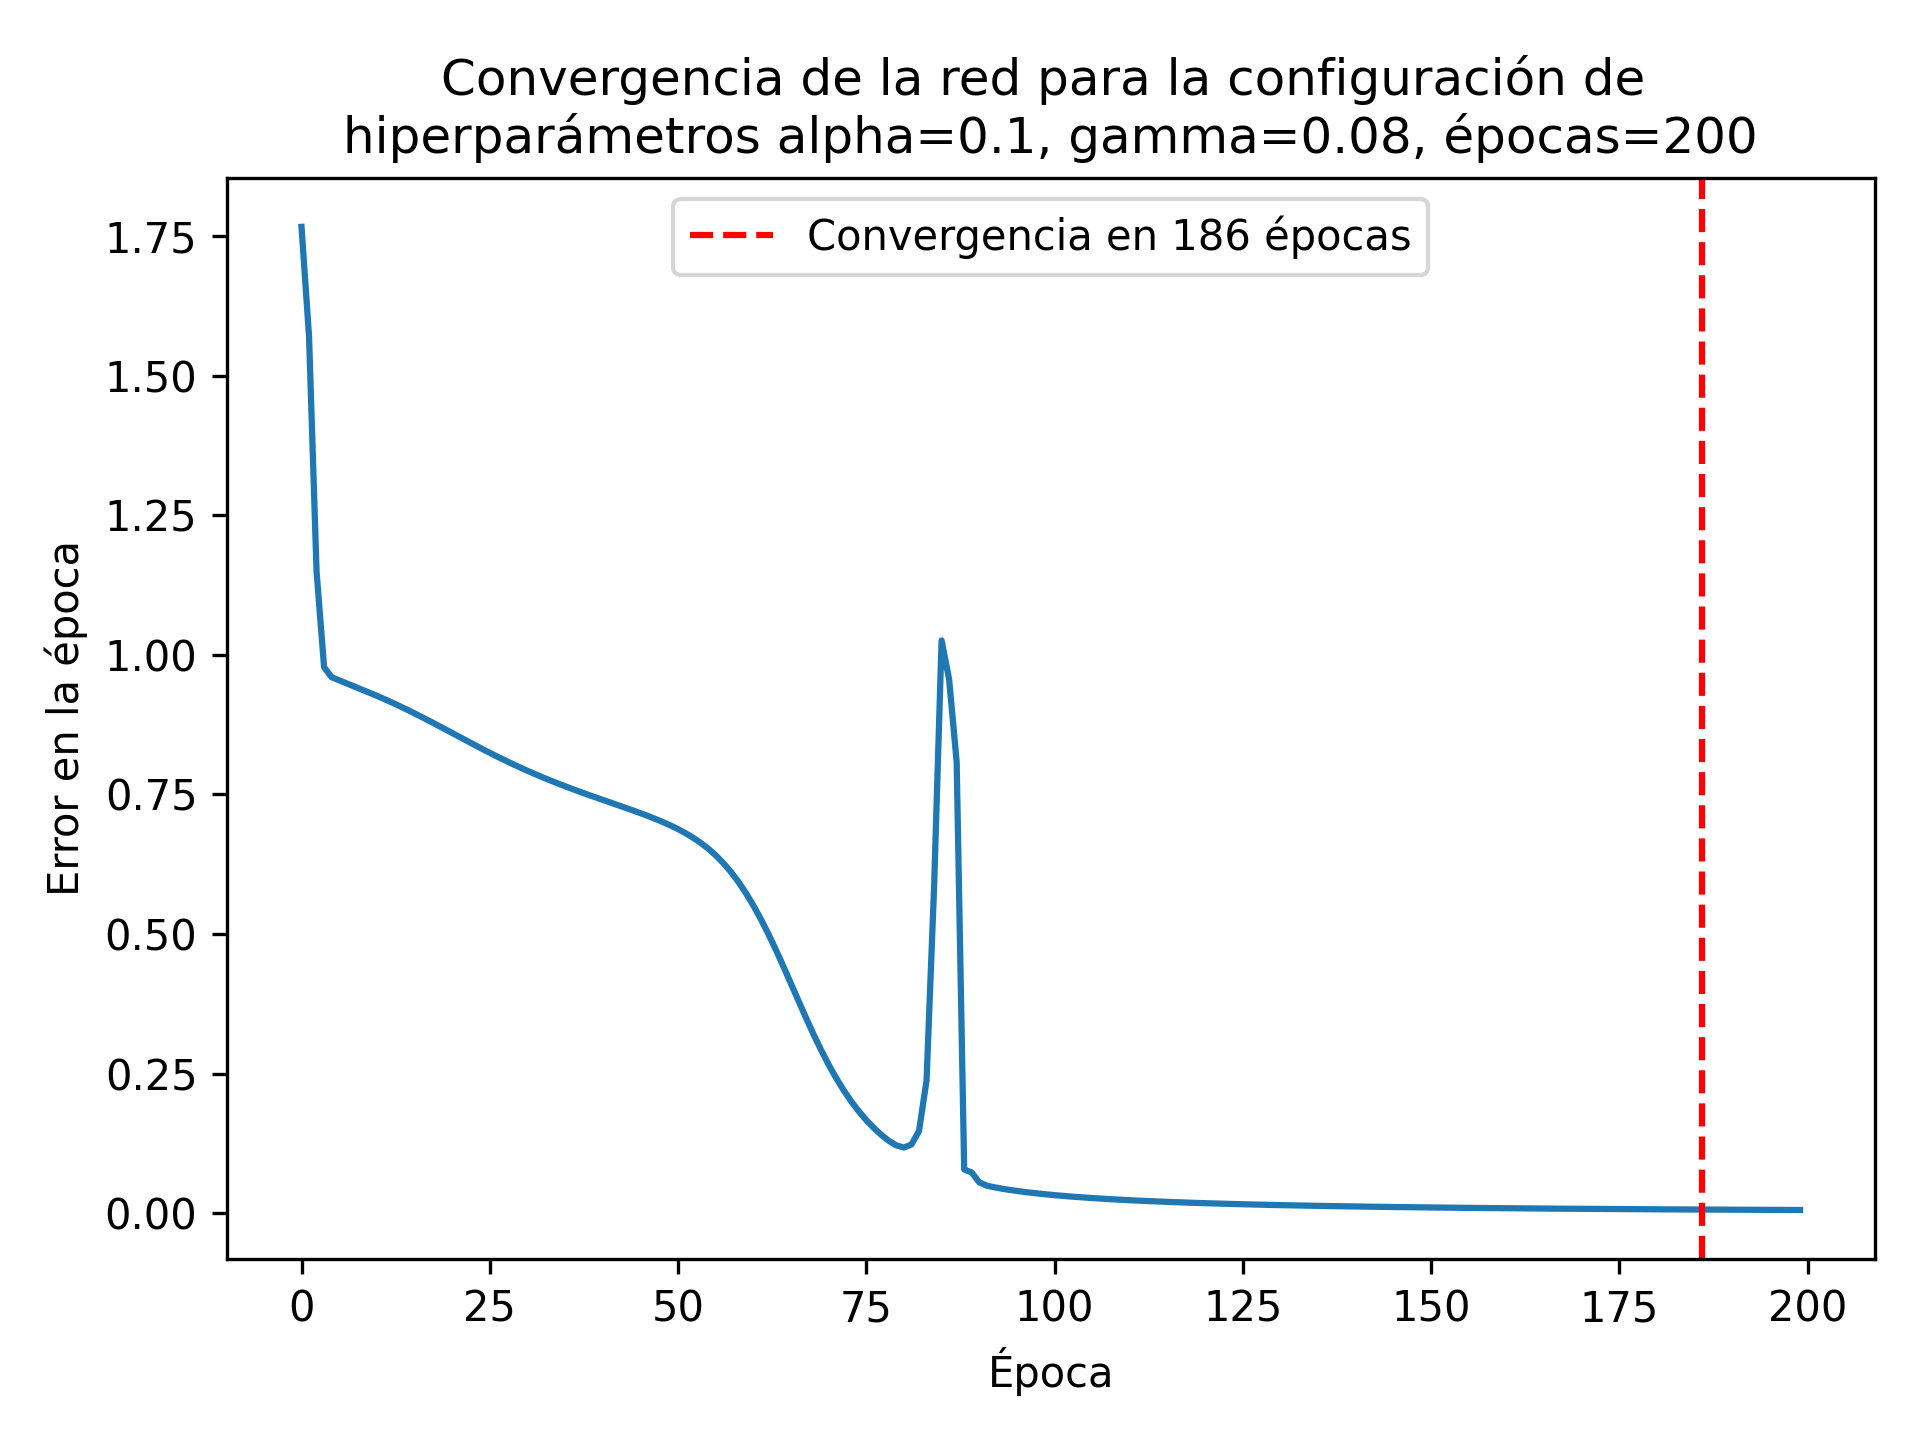
\includegraphics[width=\linewidth]{imgs/XOR/configs/convergencia_alpha_0.1_gamma_0.08_epochs_200.png}
        \caption{Convergencia de la configuración 5}
        \label{fig:conf5_xor_con}
    \end{subfigure}
    \caption{Curva de aprendizaje y convergencia para la configuración 5}
    \label{fig:conf5_lr_con_xor}
\end{figure}

\newpage
% Config 6 XOR
\begin{figure}[h!]
    \centering
    \begin{subfigure}{0.49\textwidth}
        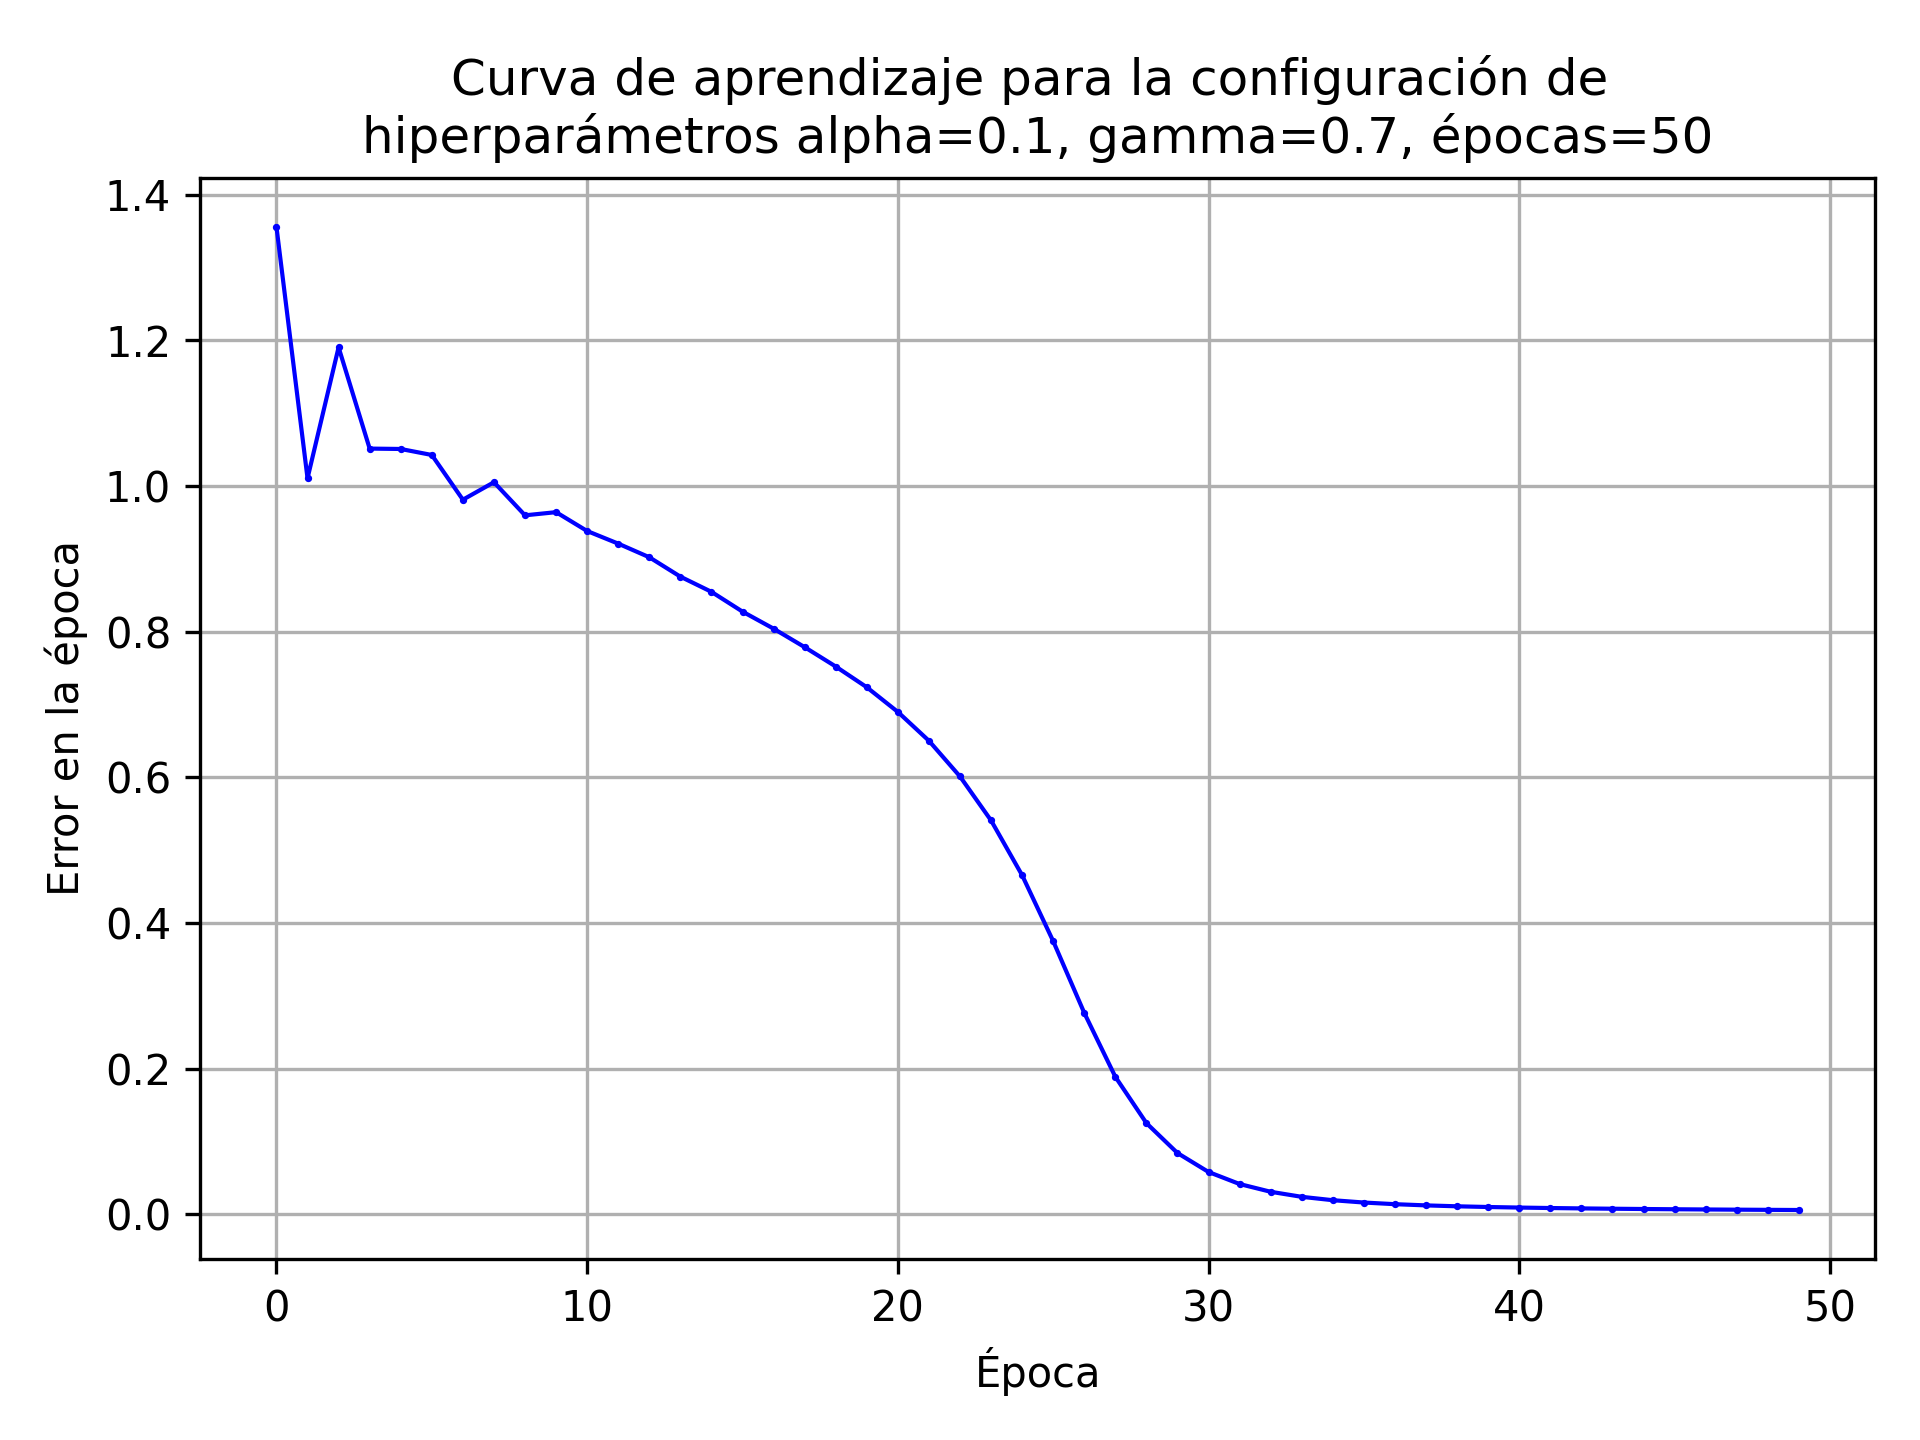
\includegraphics[width=\linewidth]{imgs/XOR/configs/curva_aprendizaje_alpha_0.1_gamma_0.7_epochs_50.png}
        \caption{Curva de aprendizaje de la configuración 6}
        \label{fig:conf_6_xor_lr}
    \end{subfigure}
    \hfill
    \begin{subfigure}{0.49\textwidth}
       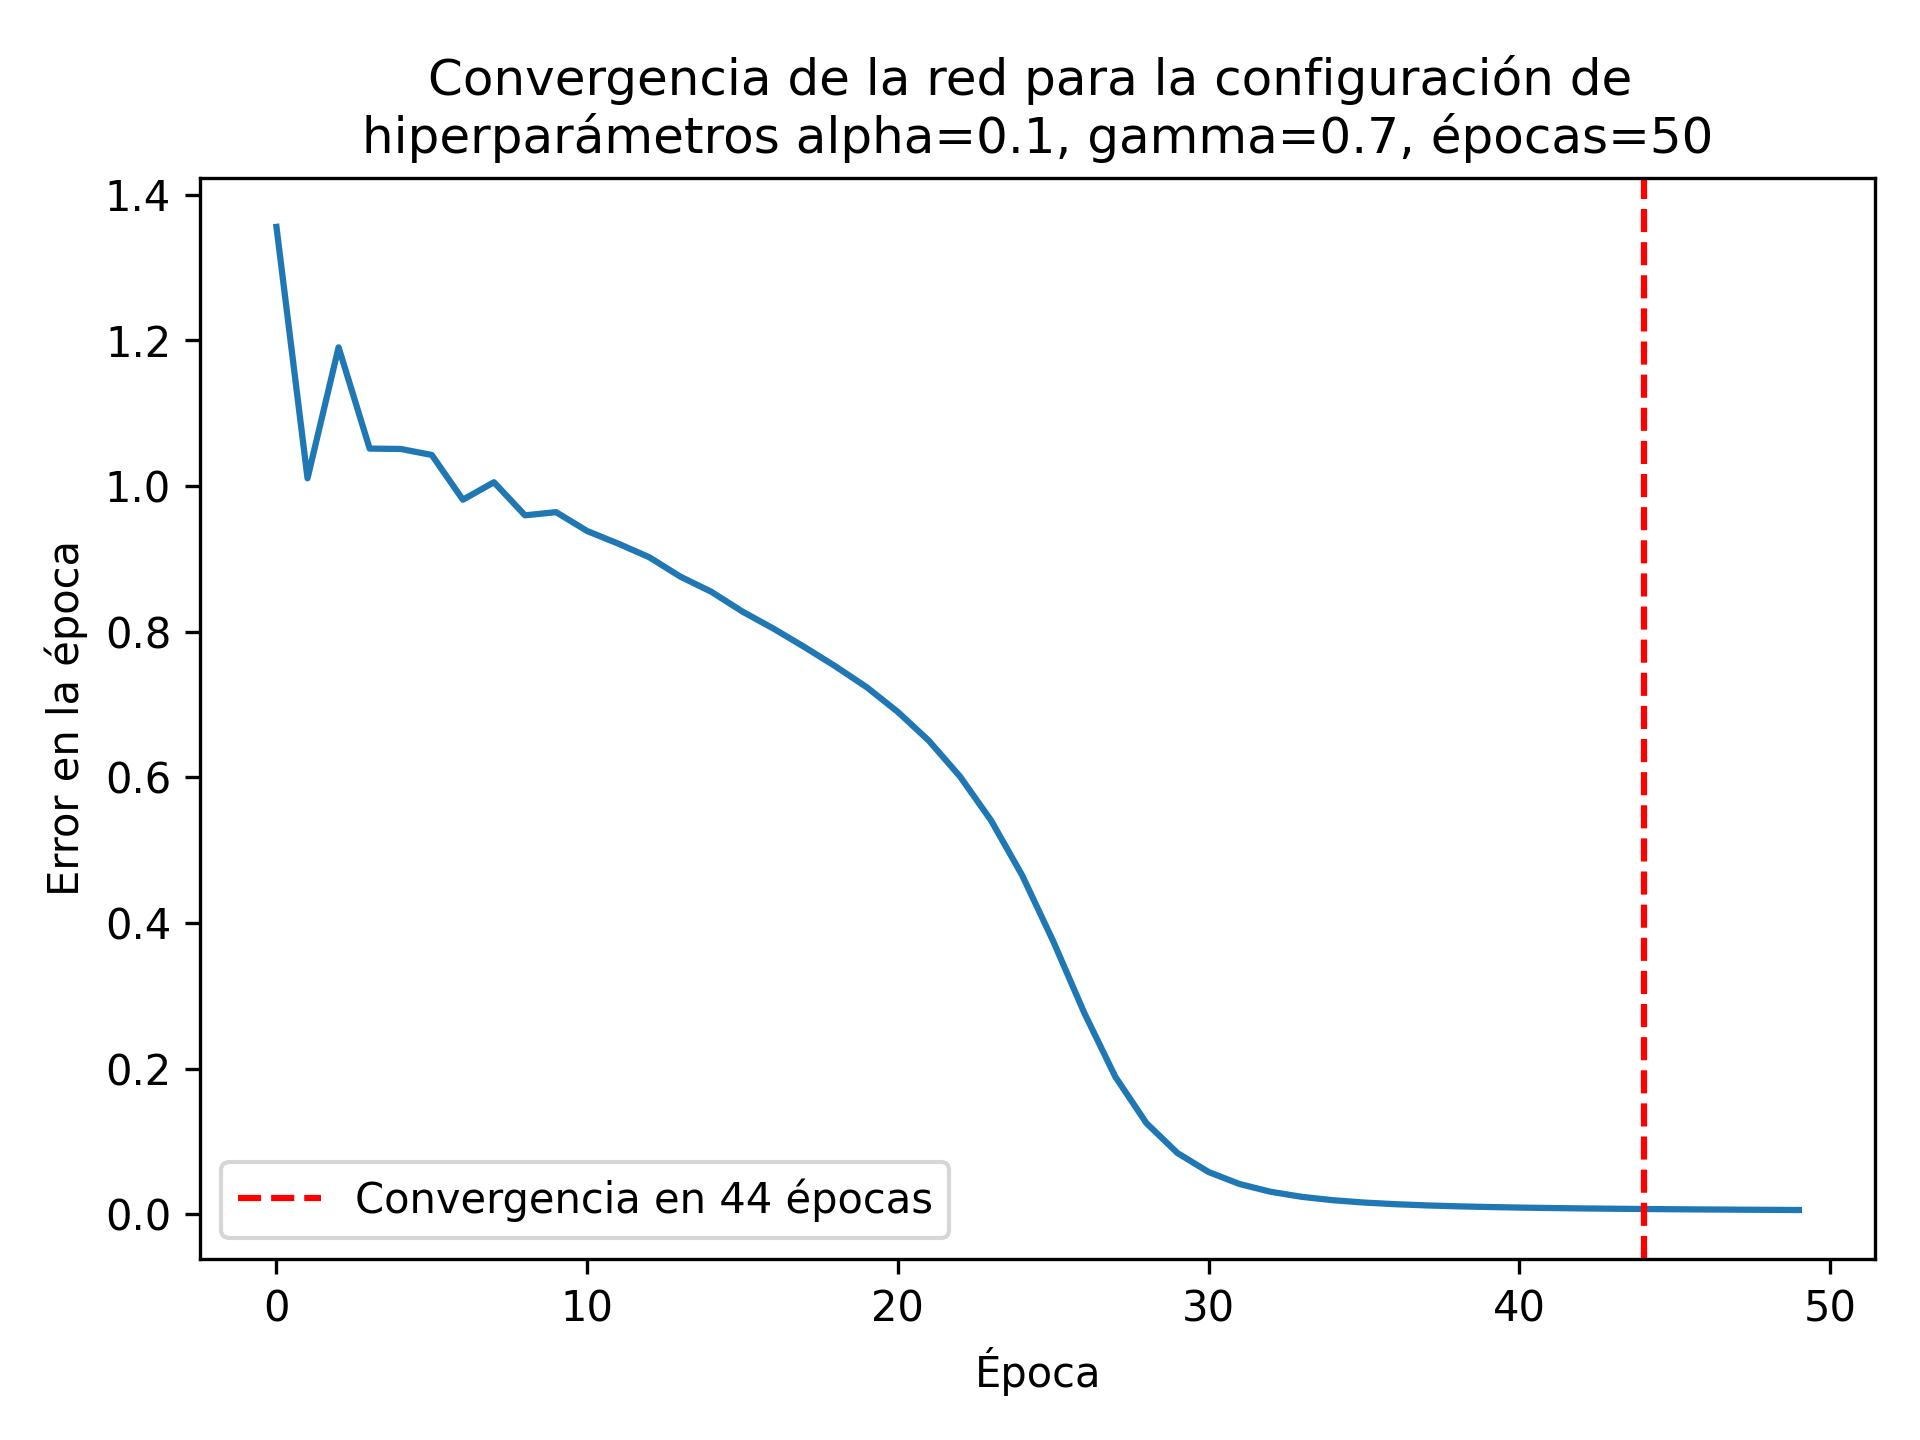
\includegraphics[width=\linewidth]{imgs/XOR/configs/convergencia_alpha_0.1_gamma_0.7_epochs_50.png}
        \caption{Convergencia de la configuración 6}
        \label{fig:conf6_xor_con}
    \end{subfigure}
    \caption{Curva de aprendizaje y convergencia para la configuración 6}
    \label{fig:conf6_lr_con_xor}
\end{figure}

% Config 7 XOR
\begin{figure}[h!]
    \centering
    \begin{subfigure}{0.49\textwidth}
        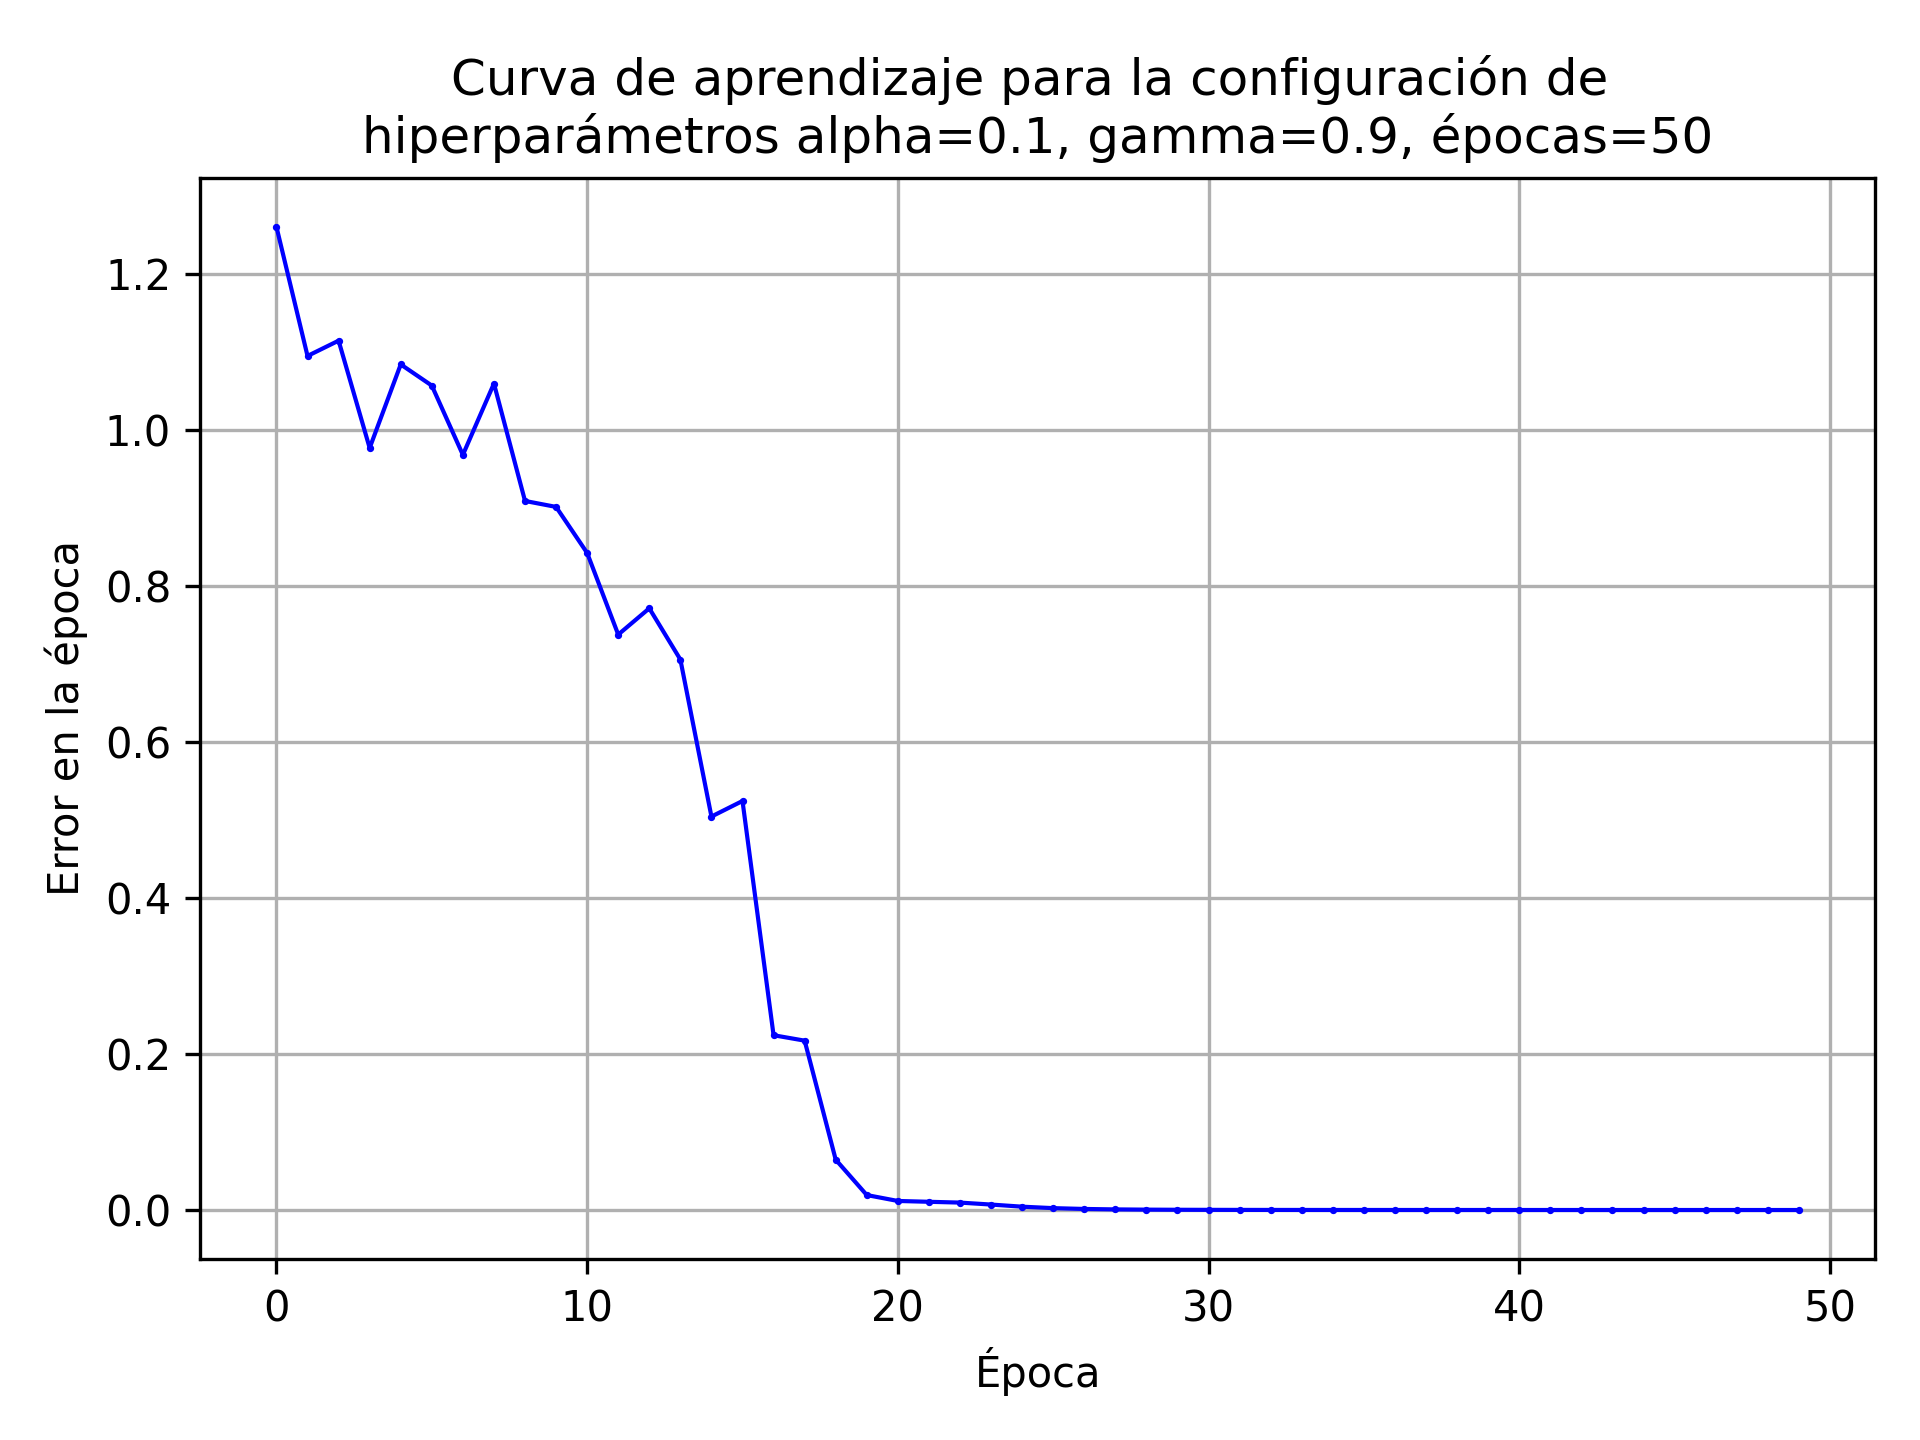
\includegraphics[width=\linewidth]{imgs/XOR/configs/curva_aprendizaje_alpha_0.1_gamma_0.9_epochs_50.png}
        \caption{Curva de aprendizaje de la configuración 7}
        \label{fig:conf_7_xor_lr}
    \end{subfigure}
    \hfill
    \begin{subfigure}{0.49\textwidth}
        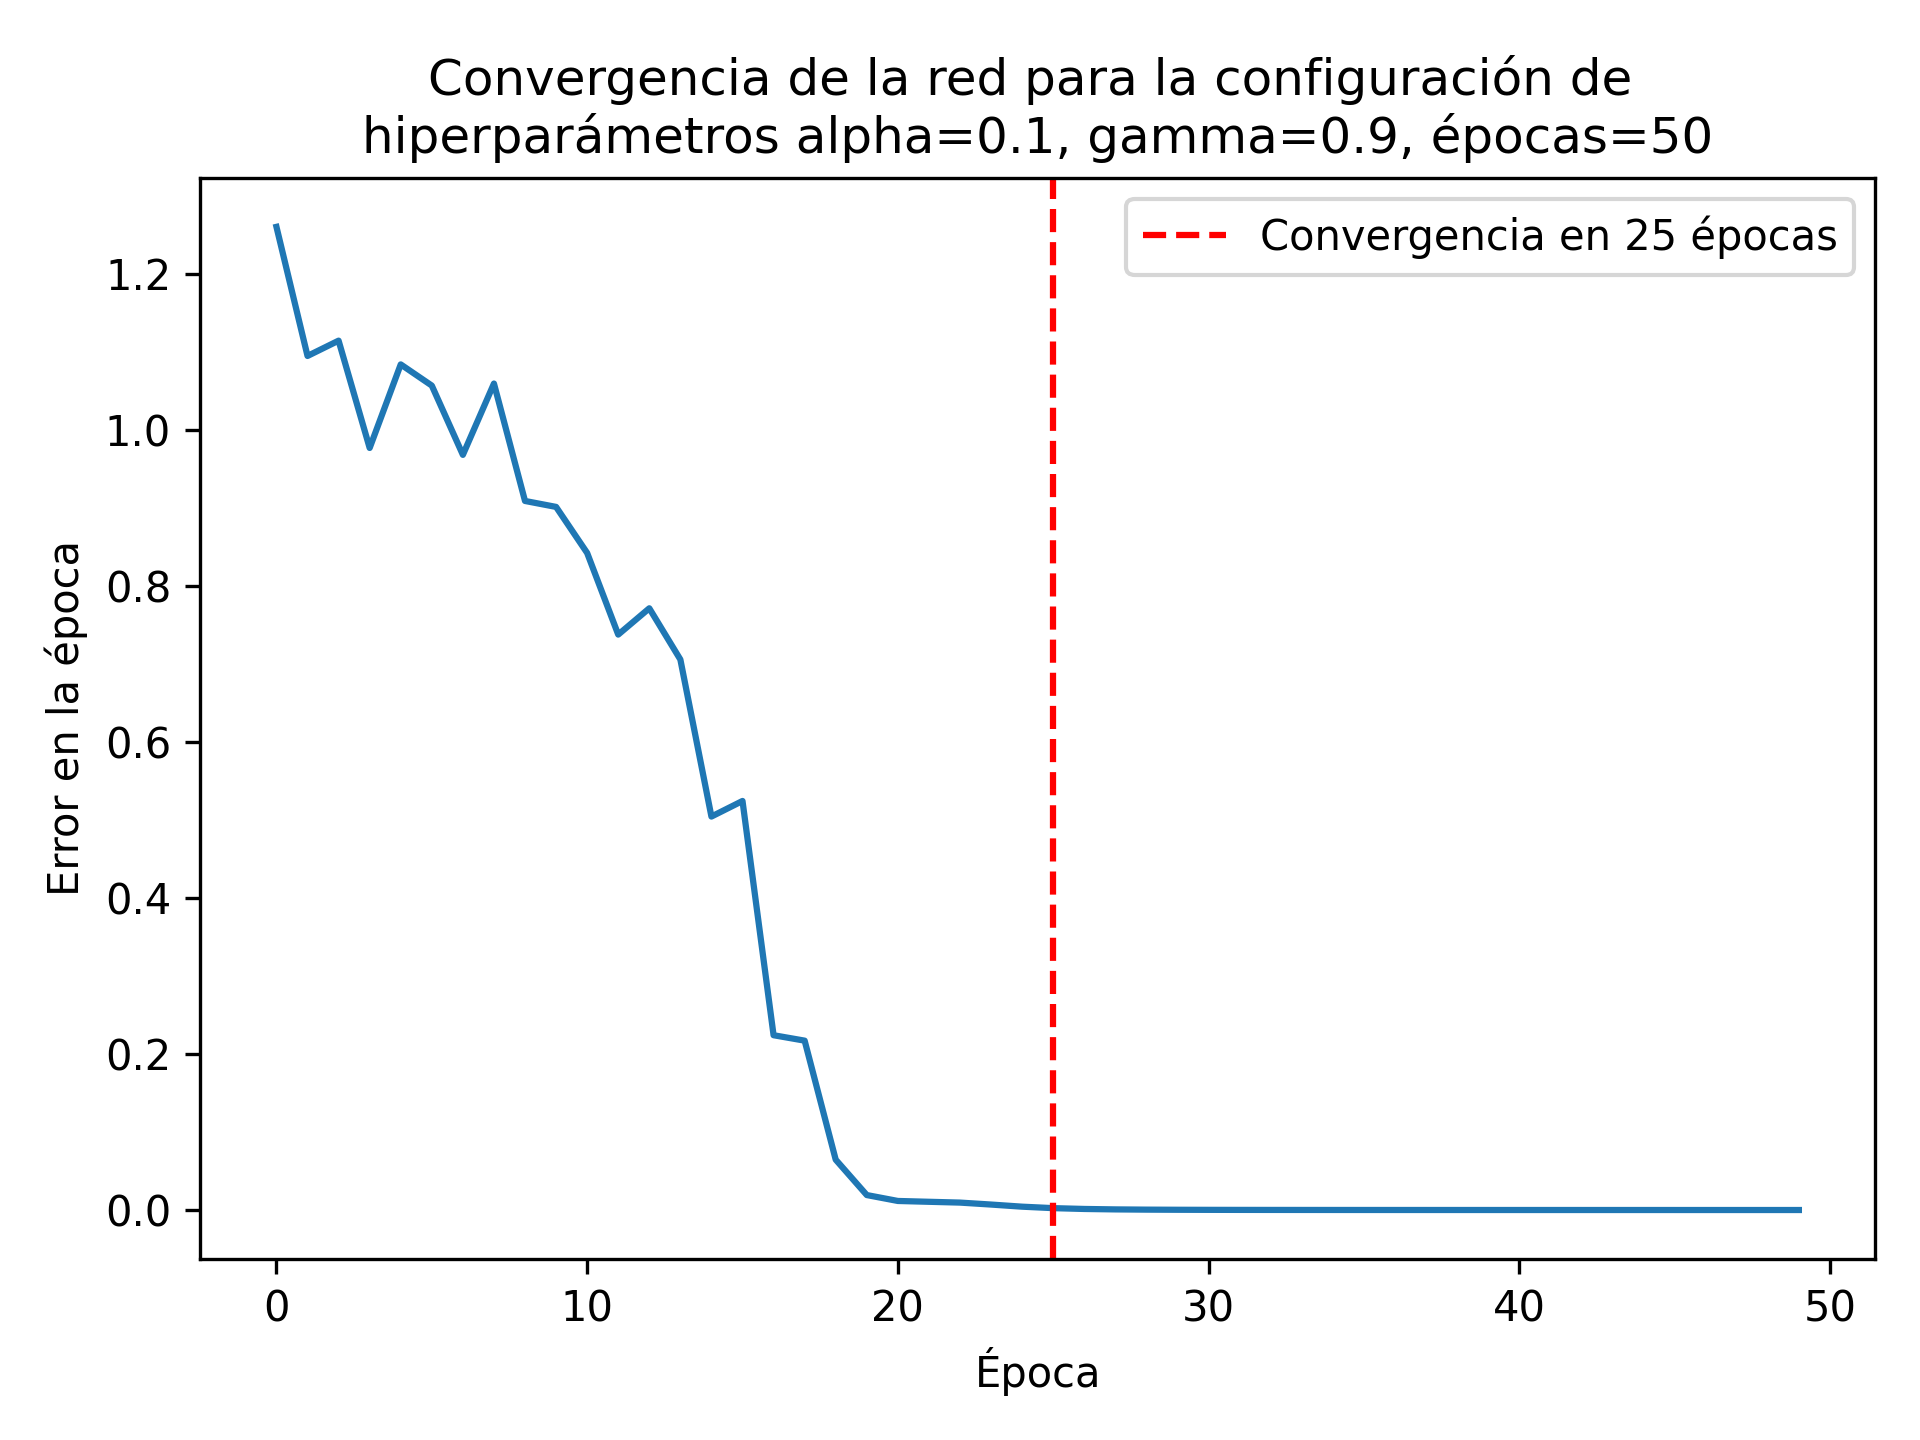
\includegraphics[width=\linewidth]{imgs/XOR/configs/convergencia_alpha_0.1_gamma_0.9_epochs_50.png}
        \caption{Convergencia de la configuración 7}
        \label{fig:conf7_xor_con}
    \end{subfigure}
    \caption{Curva de aprendizaje y convergencia para la configuración 7}
    \label{fig:conf7_lr_con_xor}
\end{figure}

Luego de las pruebas realizadas con los diferentes hiperparámetros mostrado en el cuadro \ref{tab:xor_converge_table}, se puede concluir que para el problema del XOR, un $\alpha=0.1$, es un valor bastante bueno para que la red aprenda y disminuya el error eficientemente; y además, probando diferentes configuraciones del $\gamma$, se puede controlar qué tan rápido la red converge, donde con un valor mayor, la red tiende a converger en menos de $50$ épocas. 


\newpage
\section{Clasificador de datos en $\mathbb{R}^2$}

La presente sección busca entrenar al perceptrón multicapa para clasificar datos en un espacio $\mathbb{R}^2$. Se abordarán los siguientes dos escenarios: datos que son linealmente separables y aquellos que no lo son; para ello se hará uso de la función provista \textit{generar\_datos\_R2},  para generar estos dos conjuntos de datos y posteriormente se detallará la configuración de la red para su entrenamiento.

\subsection{Generación de los dos conjuntos de datos}

Para crear conjuntos de datos sintéticos que se puedan utilizar en el entrenamiento, se emplea un enfoque basado en modelos de mezclas gaussianas (GMM). Este método permite generar datos con características estadísticamente controladas, como la media y la desviación estándar, que definen cómo se distribuyen los puntos de datos en el espacio bidimensional $\mathbb{R}^{2}$. El código implementado para la generación de datos fue brindado por el profesor del curso en el respectivo cuaderno de jupyter del trabajo práctico. 
\medskip

Para generar el conjunto de datos linealmente separables se usaron los parámetros presentados en el cuadro \ref{tab:linear_params}:
\begin{table}[h!]
    \centering
    \begin{tabular}{@{}lll@{}}
    \toprule
    Parámetro & Clase 1 & Clase 2 \\ \midrule
    Media ($\mu_1$) & $[5, 5]$ & $[19, 19]$ \\
    Desviación estándar ($\sigma_1$) & $[5, 2]$ & $[5, 2]$ \\ \bottomrule
    \end{tabular}
    \caption{Parámetros para generar datos linealmente separables}
    \label{tab:linear_params}
\end{table}

\noindent
Y de la misma forma, para generar los datos linealmente no separables, se usaron los parámetros presentados en el cuadro \ref{tab:nonlinear_params}.
\begin{table}[h!]
    \centering
    \begin{tabular}{@{}lll@{}}
    \toprule
    Parámetro & Clase 1 & Clase 2 \\ \midrule
    Media ($\mu_2$) & $[5, 8]$ & $[4, 7]$ \\
    Desviación estándar ($\sigma_2$) & $[2, 3]$ & $[2, 5]$ \\ \bottomrule
    \end{tabular}
    \caption{Parámetros para generar datos no linealmente separables}
    \label{tab:nonlinear_params}
\end{table}
\noindent
Se debe notar que para ambos conjuntos de datos se usaron $25$ observaciones por clase, es decir, cada conjunto tiene un tamaño de $50$ observaciones. Las gráficas correspondientes a cada conjunto de datos se pueden observar en la figura \ref{fig:R2_data}:

\begin{figure}[h!]
    \centering
    \begin{subfigure}{0.49\textwidth}
        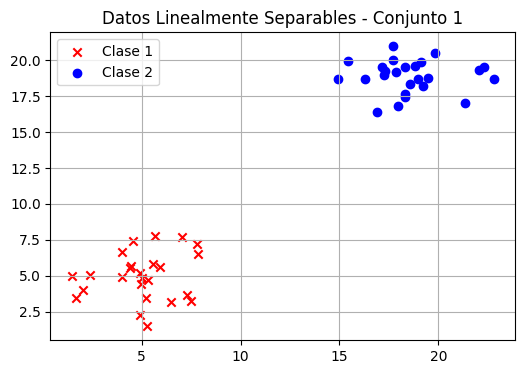
\includegraphics[width=\linewidth]{imgs/R2/data/Dataset1_lineal.png}
        \caption{Conjunto 1: Datos linealmente separables}
        \label{fig:lineal}
    \end{subfigure}
    \hfill
    \begin{subfigure}{0.49\textwidth}
       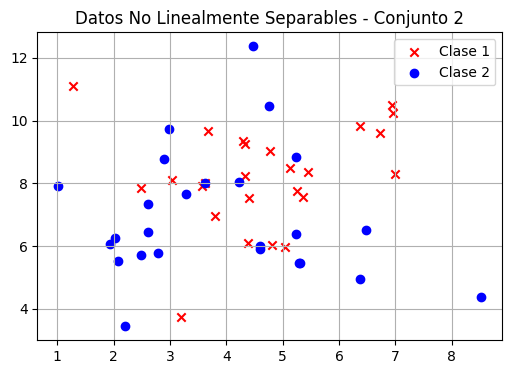
\includegraphics[width=\linewidth]{imgs/R2/data/Dataset2_no_lineal.png}
        \caption{Conjunto 2: Datos no linealmente separables}
        \label{fig:non_lineal}
    \end{subfigure}
    \caption{Gráficos de la generación de datos en $\mathbb{R}^2$.}
    \label{fig:R2_data}
\end{figure}

 

\subsection{Construcción de las redes neuronales}

Dadas las indicaciones del proyecto, se procede a detallar la construcción de cuatro redes neuronales las cuales comparten los datos: $D=2$ neuronas de entrada, y $K=1$ neuronas en la capa de salida. Las distinciones entre cada una se documentan en el cuadro \ref{tab:neural_net_arquis},

\newpage
\begin{table}[h!]
    \centering
    \begin{tabular}{@{}cccc@{}}
    \toprule
    Arquitectura & M & $\alpha$ & $\gamma$ \\ \midrule
    1 & 25 & 0.0003 & 0.5 \\
    2 & 25 & 0.001 & 0.02 \\
    3 & 4 & 0.0004 & 0.76 \\
    4 & 4 & 0.0003 & 0 \\ \bottomrule
    \end{tabular}
    \caption{Parámetros de las arquitecturas de redes neuronales}
    \label{tab:neural_net_arquis}
\end{table}

\subsection{Entrenamiento y convergencia de la red}

Dadas las arquitecturas definidas en el cuadro \ref{tab:neural_net_arquis}, se procede a entrenar cada red neuronal, tanto para el conjunto de datos linealmente separables de la figura \ref{fig:lineal}, como para el conjunto de datos no linealmente separables de la figura \ref{fig:non_lineal}, para $P=50$ iteraciones. Además, usando \textit{sklearn}, se separa cada conjunto de datos en un $80\%$ para el entrenamiento de la red, y un $20\%$ para validación. 

En el cuadro \ref{tab:r2_summary_table}, se presenta los resultados del entrenamiento para las cuatro arquitecturas creadas. Dentro del cuadro se separan en dos columnas las gráficas de los conjuntos linealmente separables y los no linealmente separables, además, cada fila representa la red neuronal detallada de la misma manera, y en el mismo orden, en el cuadro \ref{tab:neural_net_arquis}.

\newpage
% tabla de gráficas de los resultados de entrenamiento de datos en r2
\begin{table}[h!]
    \centering
    \begin{tabular}{|c|M{68mm}|M{68mm}|}
        \toprule
        Arquitectura & Linealmente separables & No linealmente separables \\
        \midrule
        1 & 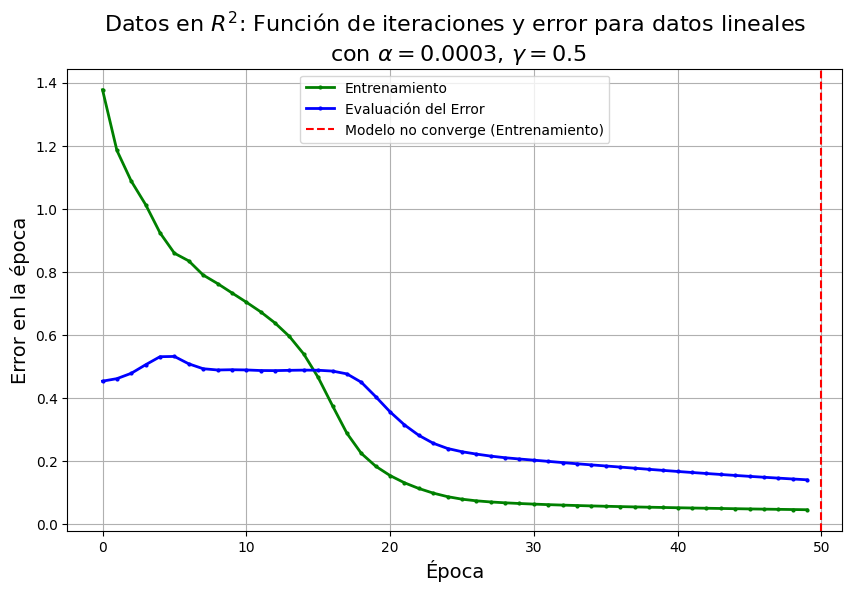
\includegraphics[width=\linewidth]{imgs/R2/Lineal_1.png} & 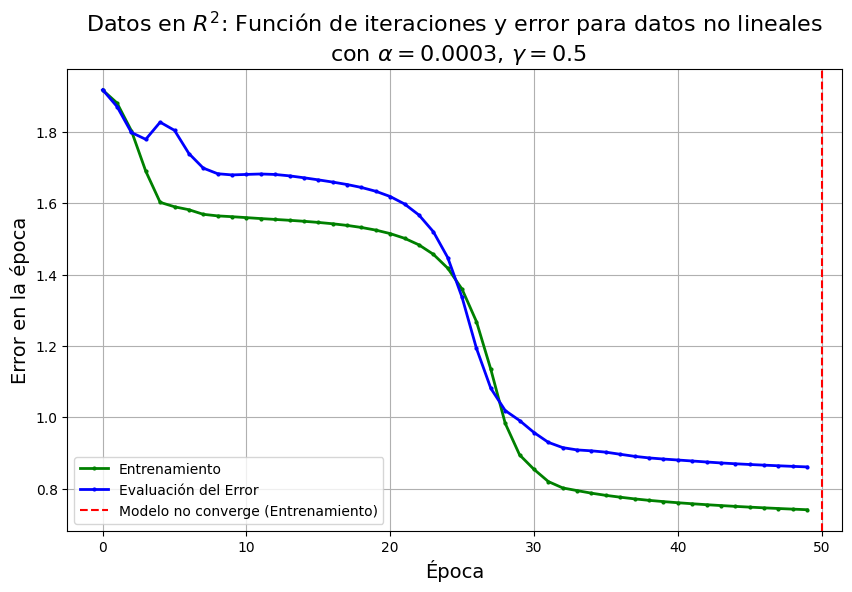
\includegraphics[width=\linewidth]{imgs/R2/Nonlineal_1.png} \\
        \hline
        2 & 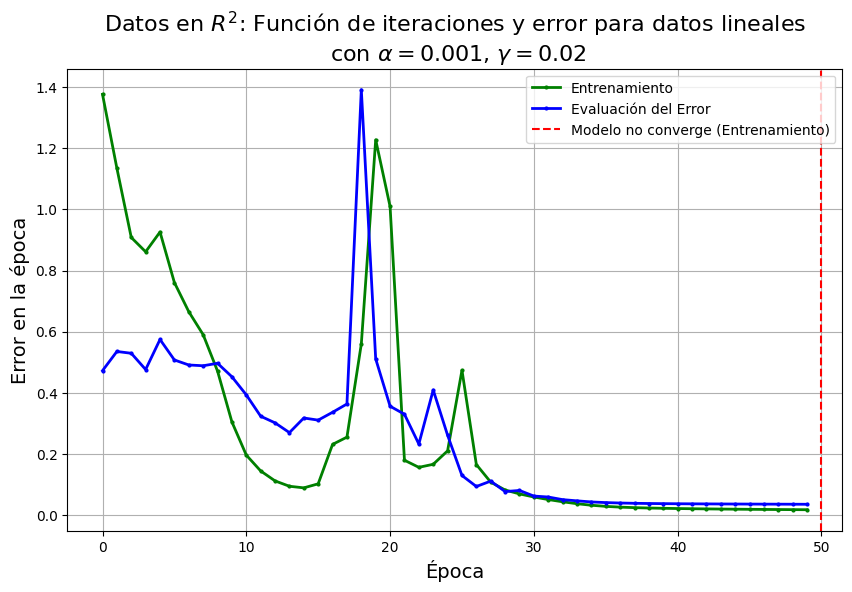
\includegraphics[width=\linewidth]{imgs/R2/Lineal_2.png} & 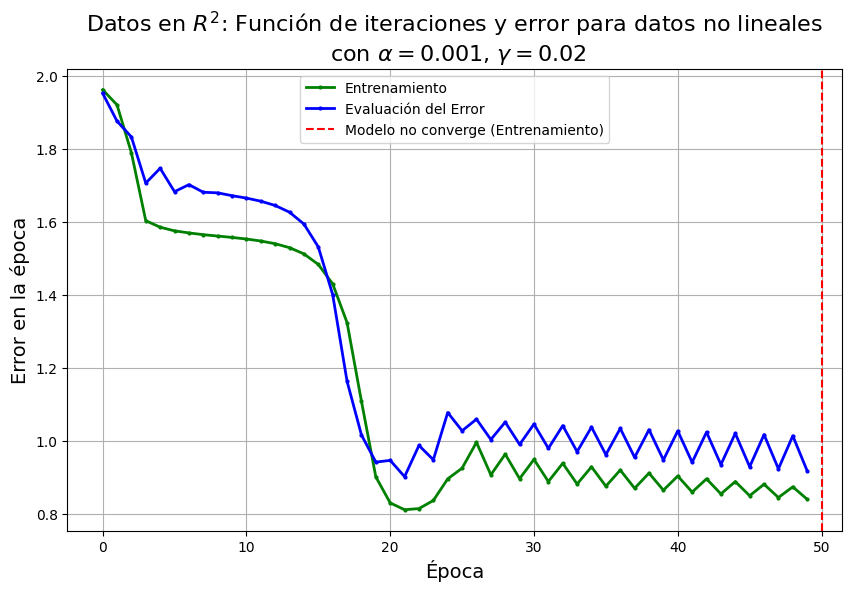
\includegraphics[width=\linewidth]{imgs/R2/Nonlineal_2.png} \\
        \hline
        3 & 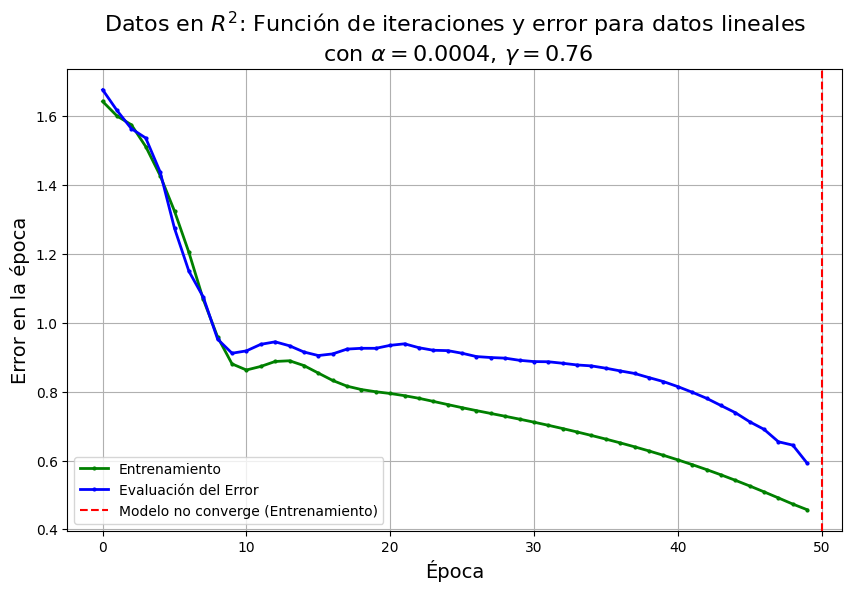
\includegraphics[width=\linewidth]{imgs/R2/Lineal_3.png} & 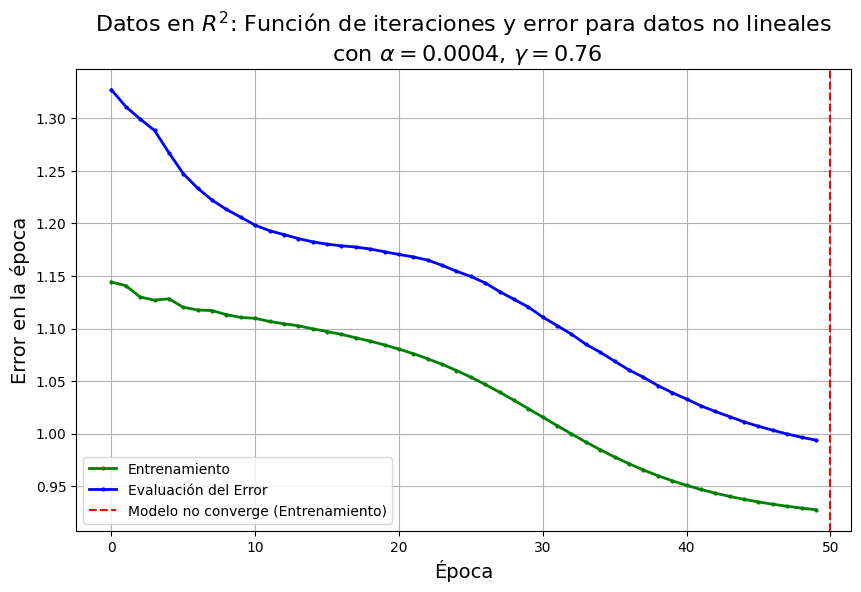
\includegraphics[width=\linewidth]{imgs/R2/Nonlineal_3.png} \\
        \hline
        4 & 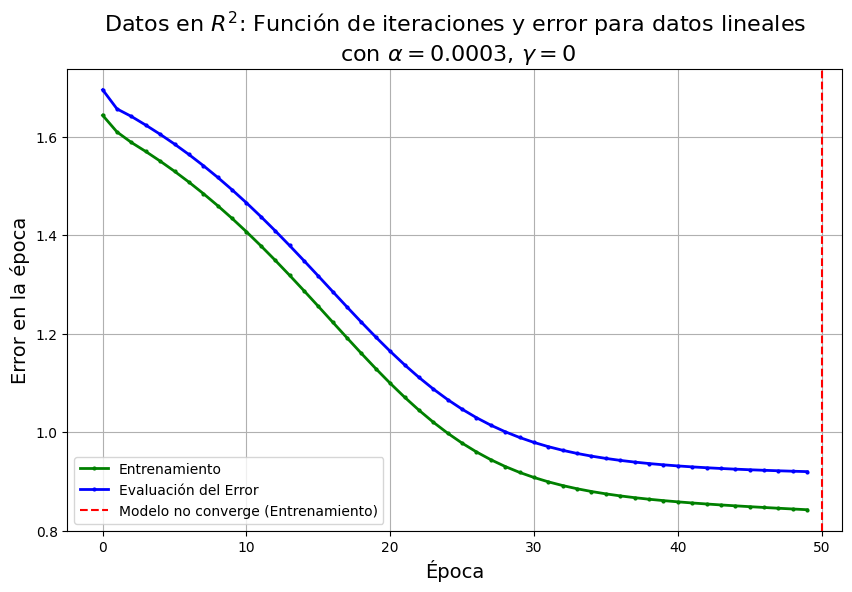
\includegraphics[width=\linewidth]{imgs/R2/Lineal_4.png} & 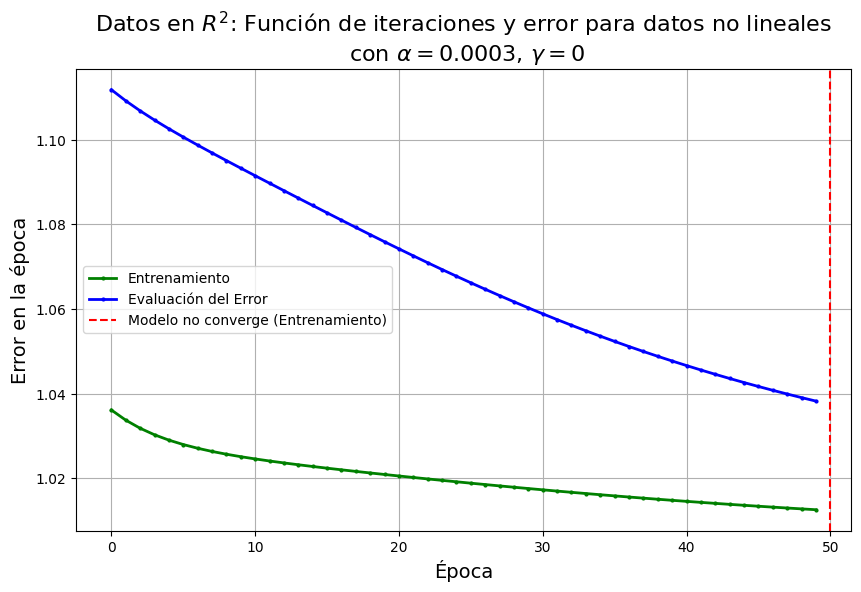
\includegraphics[width=\linewidth]{imgs/R2/Nonlineal_4.png}\\
        \bottomrule
    \end{tabular}
    \caption{Gráficas de resultado del entrenamiento para los datos en $\mathbb{R}^2$}
    \label{tab:r2_summary_table}
\end{table}

Ahora bien, en el cuadro \ref{tab:error_convergence_r2}, se detalla cada arquitectura del cuadro \ref{tab:neural_net_arquis}, junto con su error final de convergencia.

\newpage
\begin{table}[h!]
\centering
\begin{tabular}{c|c|c|c|c}
\hline
\textbf{Neuronas} & \textbf{Configuración} & \textbf{Hiperparámetros} & \textbf{Tipo} & \textbf{Loss} \\ 
\hline
\multirow{4}{*}{Neuronas {[}2, 25, 1{]}} & \multirow{2}{*}{1} & \multirow{2}{*}{$\alpha=0.0003$ , $\gamma=0.5$} & Lineal & 0.0467 \\  
 & & & No lineal & 0.7416 \\ 
 \cline{2-5}
 & \multirow{2}{*}{2} & \multirow{2}{*}{$\alpha=0.001$ , $\gamma=0.02$} &  Lineal & 0.0164 \\ 
 & & & No lineal & 0.8394 \\ 
 \hline
\multirow{4}{*}{Neuronas [2, 4, 1]} & \multirow{2}{*}{3} & \multirow{2}{*}{$\alpha=0.0004$ , $\gamma=0.76$ } & Lineal & 0.4572 \\ 
 & & & No lineal & 0.9275 \\ 
 \cline{2-5}
 & \multirow{2}{*}{4} & \multirow{2}{*}{$\alpha=0.0003$ , $\gamma=0$} & Lineal & 0.8424 \\ 
 & & & No lineal & 1.0126 \\ 
 \hline
\end{tabular}

\caption{Error final de convergencia para diferentes configuraciones}
\label{tab:error_convergence_r2}
\end{table}

Luego del entrenamiento y la obtención de resultados, los cuales son detallados tanto en el cuadro \ref{tab:r2_summary_table}, como en el cuadro \ref{tab:error_convergence_r2}, se procederá a realizar un análisis de estos. 

En primer lugar, podemos observar que, para las gráficas de la \textbf{configuración 1}, tanto para los datos lineales, como los no lineales, la red pareciera que se aproxima a una convergencia, al menos para los datos lineales, los cuales presentan un error final de $0.0467$, pero que al mismo tiempo, los datos no lineales siguen una misma tendencia donde su error baja de una manera similar pero un poco más lenta. Para esta configuración se usan 25 neuronas en la capa oculta, junto con un $\alpha=0.0003$ y un $\gamma=0.5$. 

La \textbf{configuración 2} es un poco similar a la \textbf{configuración 1}, no obstante, se usa un $\alpha$ más grande, lo que pareciera que, para los datos lineales, ayuda a mejorar la convergencia, pero que para los no lineal, no existe un cambio muy significativo. 

Ahora bien, para la \textbf{configuración 3} y \textbf{configuración 4}, se usa menos neuronas en la capa oculta, pero de la misma manera, se sigue usando un $\alpha$ muy similar a la \textbf{configuración 1}. Con esta combinación se puede notar que el error final de convergencia es mucho mayor para los datos lineales y no lineales. 

Con estos resultados se puede decir que la cantidad de neuronas en la capa oculta afecta a la convergencia de la red de una manera bastante significativa, que además, donde a mayor número de neuronas, un $\alpha$ más pequeño es necesario, esto debido a que, si se observa las gráficas del cuadro \ref{tab:r2_summary_table}, se puede ver una diferencia muy grande entre las gráficas de las primeras dos filas, con las filas 3 y 4. Donde las primeras dos filas presentan una convergencia más cercana a 0 que las otras dos. Dada la complejidad de los datos no lineales, quizás se presenta lo que se conoce como \textbf{under fitting} \cite{panchal2011behaviour} en la red neuronal. Y de igual manera, el presentar una enorme cantidad de neuronas en la capa oculta, puede llevar a un \textbf{sobreajuste} o incluso que se tome una gran cantidad de tiempo para procesar los datos \cite{panchal2011behaviour}. 

Para lidiar con los problemas mencionados anteriormente, existen métodos para escoger la cantidad correcta de neuronas en la capa oculta. Un punto de inicio puede ser:
\begin{itemize}
    \item El número de neuronas de la capa oculta debería estar entre el tamaño de la capa de entrada y el tamaño de la capa de salida.
    
    \item El número de neuronas de la capa oculta debería ser 2/3 del tamaño de la capa de entrada, más el tamaño de la capa de salida.
    
    \item  El número de neuronas de la capa oculta debería ser menor que el doble del tamaño de la capa de entrada. \cite{panchal2011behaviour}
\end{itemize}

Si nos basamos en alguno de los puntos anteriores, por ejemplo, segundo punto, podríamos entonces escoger un número de neuronas para la capa oculta de la siguiente manera:

\begin{equation*}
    M = \frac{2}{3} (D+K),
\end{equation*}

Para nuestro caso, tenemos que, $D=2$ y $K=1$, por ende:
\begin{align*}
    M &= \frac{2}{3}(2+1)\\
    M &= \frac{2}{3} \cdot 3 \\
    M &= 2
\end{align*}

Entonces se puede decir que, existen métodos para poder determinar el número de neuronas en la capa oculta dado el número de neuronas en la capa de entrada. Además, el coeficiente de aprendizaje $\alpha$ es dependiente del número de neuronas en la capa oculta de igual manera, ya que, de usar un menor número de neuronas, se puede tomar un $\alpha$ inclusive más pequeño, esto para que el modelo no realice 'saltos' muy grandes en la búsqueda de un mínimo. 


\newpage

\newpage
\section{Clasificador de ataques usando datos estructurados}

La presente sección busca entrenar al perceptrón multicapa para clasificar datos estructurados obtenidos del dataset \textit{UNSW-NB15: A Comprehensive Data set for Network Intrusion Detection systems}, codificando los datos mediante la técnica \textit{One-Hot Vector}. Para ello, fue necesario preparar los datos a través de la biblioteca Pandas, tomando de referencia códigos de ejemplo brindados por el profesor del curso. En la presente sección se cubrirá el procesamiento de los datos y el entrenamiento respectivo.

\subsection{Procesamiento de datos para la codificación}

Para realizar el procesamiento de los datos, se utilizó la biblioteca \texttt{Pandas}, que brinda herramientas para para importar el dataset y transformarlo de manera tal que se utilicen únicamente datos relevantes para el ejercicio, así como modificar la cardinalidad de algunas características con el fin reducir las características codificadas para el método \textit{one hot vector.}

\begin{figure}[htbp]
\begin{lstlisting}[language=Python, texcl=True]
import numpy as np
import pandas as pd

# Carga de los datos
df = pd.read_csv('/content/UNSW_NB15_training-set.csv')

# Elimina columnas no necesarias
list_drop = ['id','attack_cat']
df.drop(list_drop, axis=1,inplace = True)

# Descripción de datos categóricos
df.describe(exclude=np.number)
\end{lstlisting}
\caption{Carga de datos del dataset en un dataframe.}
\label{code:dataframes}
\end{figure}

En la figura \ref{code:dataframes} se muestra como se cargaron los datos del dataset completo, además en la línea 12 se realiza un filtro donde se seleccionan únicamente registros categóricos al excluir datos numéricos, a continuación en el cuadro \ref{tab:df_cat_describe} se puede ver una descripción de dichas variables.

\begin{table}[htbp]
    \centering
    \begin{tabular}{llll}
    \toprule
     & proto & service & state \\
    \midrule
    count & 82332 & 82332 & 82332 \\
    unique & 131 & 13 & 7 \\
    top & tcp & - & FIN \\
    freq & 43095 & 47153 & 39339 \\
    \bottomrule
    \end{tabular}
    \caption{Descripción de los datos categóricos del dataframe.}
    \label{tab:df_cat_describe}
\end{table}

Del cuadro anterior, se puede evidenciar cómo las tres categorías tienen 82332 registros y la categoría ``\texttt{proto}'' (protocolo) es quién más tipos de valores únicos presenta, la intención es reducir la cantidad de valores únicos previo a la codificación \textit{one hot vector}. Para ello se implementará la siguiente estrategia:

\begin{itemize}
    \item Preservar sólo aquellos registros con valores dentro del top 5 de los valores más frecuentes del dataset. Esto realizado con los métodos \texttt{value\_counts() y head()}, que retornan, respectivamente; una array ordenado de mayor a menor con la suma de datos por categoría, y los primeros cinco datos del array anterior.

    \item Reemplazar con ``-'' si el valor no está entre el top 5 más frecuente
\end{itemize}

\newpage
Con estas estrategias se reduce significativamente la cantidad de valores únicos, debido a que se conservan sólo aquellos que sean parte del top 5 más frecuente, a continuación, el código implementado que realiza la reducción:

\begin{figure}[htbp]
\begin{lstlisting}[language=Python, texcl=True]
# Filtrar solo pro datos categóricos
df_cat = df.select_dtypes(exclude=[np.number])

for feature in df_cat.columns:
    if df_cat[feature].nunique() > 5:
        df[feature] = np.where(df[feature].isin(top5.index), df[feature], '-')

df.describe(exclude=np.number)
\end{lstlisting}
\caption{Reducción de los valores únicos de las categorías según su top5 de datos más frecuentes.}
\label{code:reducted_df}
\end{figure}

Una vez hecha la reducción de la figura \ref{code:reducted_df}, podemos nuevamente mostrar la descripción  de los datos categóricos y evidenciar una notoria reducción de sus valores únicos, la cuál se muestra continuación:

\begin{table}[htbp]
    \centering
    
    \begin{tabular}{llll}
    \toprule
     & proto & service & state \\
    \midrule
    count & 82332 & 82332 & 82332 \\
    unique & 6 & 5 & 6 \\
    top & tcp & - & FIN \\
    freq & 43095 & 49275 & 39339 \\
    \bottomrule
    \end{tabular}

    \caption{Descripción de los datos categóricos del dataframe con valores únicos reducidos.}
    \label{tab:df_reduced}
\end{table}

Nótese del cuadro \ref{tab:df_reduced} que ahora la cantidad de valores únicos para las características categóricas del dataset son mucho menores que en el cuadro \ref{tab:df_cat_describe}.

\subsection{Codifiación one hot vector}

Para realizar codificación se utilizó la biblioteca \texttt{scikit-learn}, que brinda herramientas para utilizar un transformador que convierte variables categóricas en una representación numérica, que es más adecuada para modelos de aprendizaje automático, creando una nueva variable binaria para cada categoría.

\begin{figure}[htbp]
\begin{lstlisting}[language=Python, texcl=True]
from sklearn.compose import ColumnTransformer
from sklearn.preprocessing import OneHotEncoder

# X representa las categorías a codificar, Y representa los targets
X = df.iloc[:,:-1]
y = df.iloc[:,-1]

# Crear el transformador one-hot encoder y transforma los datos
transform_columns = [1, 2, 3]
ct = ColumnTransformer(transformers=[('encoder',OneHotEncoder(), transform_columns)],
                       remainder='passthrough'
     )
X = np.array(ct.fit_transform(X))
\end{lstlisting}
    \caption{Implementación de la codificación One Hot vector}
    \label{code:oneHotEncoder}
\end{figure}

En la figura \ref{code:oneHotEncoder} se crea una instancia de ColumnTransformer, dicha instancia está configurada para aplicar la codificación \texttt{OneHotEncoder} a las columnas especificadas (índices 1, 2 y 3 del DataFrame X). Las columnas que no están especificadas para ser transformadas por el OneHotEncoder serán dejadas intactas gracias al parámetro \texttt{remainder="passthrough"}. Esto significa que las columnas no listadas en los índices [1, 2, 3] se añadirán sin cambios al resultado final tras la transformación. Luego, el resultado de \texttt{ct.fit\_transform(X)} se convierte a un array de NumPy para posiblemente facilitar operaciones futuras, dado que muchos algoritmos en scikit-learn esperan datos en este formato.

\subsubsection{Procesamiento de datos para entrenar el modelo}

Una vez obtenida la codificación, es necesario ajustar los datos para empezar el entrenamiento, estos ajustes constan de convertir a tensores los datos obtenidos DataFrame X, agregar una columna de 1's al inicio para el sesgo y cambiar los valores en 0 por -1. A continuación el código implementado para ello:

\begin{figure}[htbp]
\begin{lstlisting}[language=Python, texcl=True]
from sklearn.model_selection import train_test_split

def add_ones_column(input):
    ones_column = np.ones((input.shape[0], 1))
    return torch.tensor(np.hstack((ones_column, input)), dtype=torch.float)

def swap_zeros(input):
    input = torch.tensor(input.values, dtype=torch.float)
    input[input == 0] = -1
    return input.unsqueeze(1)

# Dividir los datos en conjuntos de entrenamiento y validación
# Se usa el 80\% para entrenar el modelo y el 20\% para evaluarlo el modelo
data = train_test_split(X, y, test_size = 0.2, random_state = 0, stratify=y)
X_train, X_test, T_train, T_test = data

# Crear una columna de unos
X_train = add_ones_column(X_train)
X_test = add_ones_column(X_test)

# Cambiar 0 por -1
T_train = swap_zeros(T_train)
T_test = swap_zeros(T_test)
\end{lstlisting}
\caption{Procesamiento de datos previo al entrenamiento con el modelo}
\label{code:cleaning_data}
\end{figure}

Para concluir, de la figura \ref{code:cleaning_data}, puede verse como nuevamente, al igual que en los otros entrenamientos realizado, se utiliza una relación de 80-20 para entrenamiento y pruebas, en la siguiente sección se detalla el entrenamiento a realizar.


\subsection{Entrenamiento de la red}

Dadas las indicaciones del presente trabajo, es necesario ahora definir la cantidad de neuronas $D$ que tendrá la capa de entrada, así como la cantidad de neuronas $K$ que tendrá la capa de salida, para ello se estudiaron las dimensiones de los datos, y se tomó la decisión de tomar $D=57$ neuronas de entrada, siendo 57 el número de columnas de los datos, y $K=1$ fue decido dadas las recomendaciones vistas en clase. A continuación se muestra los parámetros de la red y la magnitud de error mínima alvanzada:


\begin{table}[htbp]
    \centering
    \begin{tabular}{@{}cccc@{}}
    \toprule
    Neuronas {[}D, M, K{]} &  $\alpha$ & $\gamma$ & Loss \\ \midrule
    {[}57, 17, 1 {]} & $1e^{-7}$ & 0 & 0.9929 \\ \bottomrule
    \end{tabular}
    \caption{Error final de convergencia para el entrenamiento de datos estructurados}
    \label{tab:structured_params}
\end{table}

De acuerdo a la tabla \ref{tab:structured_params}, se muestra ahora la gráfica de los errores a través de las 50 épocas de entrenamiento:

\begin{figure}[htbp]
    \centering
    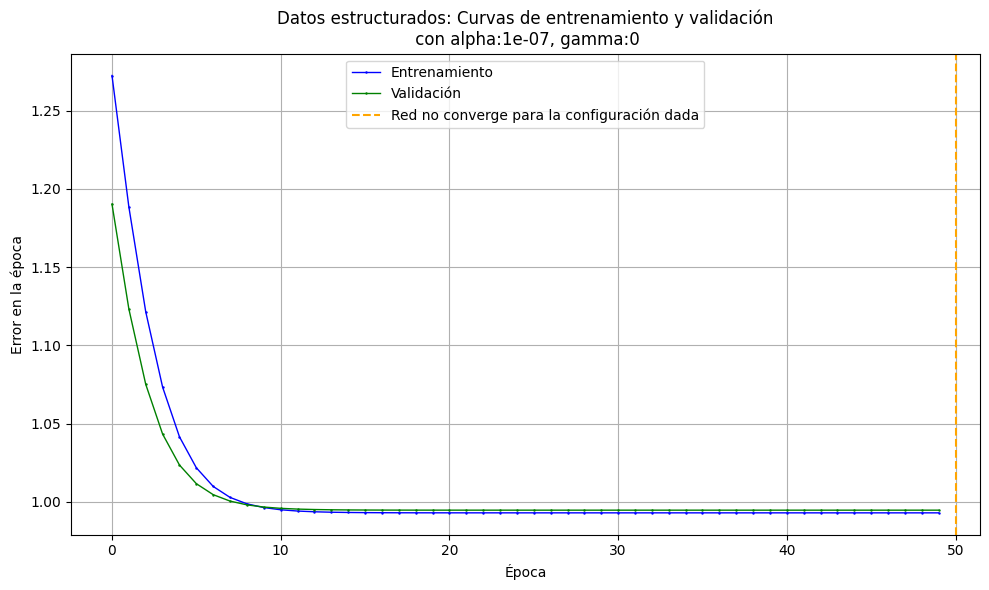
\includegraphics[width=0.65\linewidth]{imgs/structured/structured_data.png}
    \caption{Errores a través de 50 épocas del entrenamiento con datos estructurados}
    \label{fig:test}
\end{figure}


Como se puede evidenciar en la figura \ref{fig:test}, los errores parecen acercarse a cero desde la época 10 o inclusive antes, esto muestra como el perceptrón implementado fue capaz de aprender de este conjunto de datos de manera satisfactoria.


\subsection{Optimización de hiper-parámetros con optuna}

Adicionalmente al entrenamiento se decidió implementar una optimización de hiper-parámetros con la biblioteca optuna, el cuál fue implementado de la siguiente forma:

\begin{figure}[htbp]
    \centering
    \begin{lstlisting}[language=Python, texcl=True]
def objective(trial):
    # Generar candidatos de hiperparámetros con Optuna
    D = X_train.shape[1]
    M = trial.suggest_int('M', 1, 20)  # Número de neuronas en la capa oculta
    alpha = trial.suggest_float('alpha', 1e-10, 1e-1, log=True)
    gamm = 0
    params = [M, alpha, gamm]

    # Creamos y entrenamos el modelo con los parámetros seleccionados
    _, errors_train, errors_test, epoch_converge = train_structured_data(50, X_train, T_train, X_test, T_test, params, print_e=False)

    # Minimizamos el error de validación final
    return errors_train[-1]  # suponiendo que errors\_test contiene el error de validación en cada época

# Definir el estudio de Optuna y número de trials
study = optuna.create_study(direction='minimize')
study.optimize(objective, n_trials=100)
    \end{lstlisting}
    \caption{Optimización de hiper-parámetros con optuna}
    \label{fig:optuna}
\end{figure}


Como resultado de haber realizado un entrenamiento por 100 intentos, de la figura \ref{fig:optuna} se obtuvieron los siguientes mejores parámetros parámetros y pérdida:

\begin{table}[htbp]
    \centering
    \begin{tabular}{@{}cccc@{}}
    \toprule
    Neuronas {[}D, M, K{]} &  $\alpha$ & $\gamma$ & Loss \\ \midrule
    {[}57, 3, 1 {]} & $1.4025e^{-6}$ & 0 & 0.9899  \\ \bottomrule
    \end{tabular}
    \caption{Error final de convergencia para el entrenamiento de datos estructurados}
    \label{tab:obtuna}
\end{table}

Nótese que hay una ligera diferencia entre los errores mínimos del cuadro \ref{tab:structured_params} y el cuadro \ref{tab:obtuna}. Siendo  del segundo cuadro un error menor el resultante de los parámetros con optuna. Cabe mencionar que existe una significativa diferencia entre los valores de M, siendo ahora 14 veces menor, esto repercute en la cantidad de pasos necesarios para calcular los resultados, ya que, al ser menos dimensiones son menos multiplicaciones.

\newpage
\subsection{Normalización de los datos de entrada}

Se realizó la normalización de 0 a 1, utilizando el valor máximo de la observación, esto calculado de la siguiente forma:

\begin{figure}[htbp]
    \centering
    \begin{lstlisting}[language=Python, texcl=True]
ef normalize_data(X):
    # Asegura que X es un tensor de PyTorch
    X = torch.as_tensor(X, dtype=torch.float32)
    
    # Calcula el valor máximo por observación (a lo largo de cada fila si X es una matriz 2D)
    X_max = X.abs().max(dim=1, keepdim=True)[0]
    
    # Evita la división por cero ajustando los valores máximos que sean cero a uno
    X_max[X_max == 0] = 1
    
    # Normaliza los datos
    return X / X_max

P = 30

# Normalizar los datos de entrenamiento y prueba
X_train_norm = normalize_data(X_train)
X_test_norm = normalize_data(X_test)

M = study.best_trial.params["M"] # número de neuronas en la capa oculta
alph, gamm = study.best_trial.params["alpha"], 0
params = [M, alph, gamm]

train = train_structured_data(P, X_train, T_train, X_test, T_test, params, print_e=False)
train_norm = train_structured_data(P, X_train_norm, T_train, X_test_norm, T_test, params, print_e=False)
    \end{lstlisting}
    \caption{Normalización de los datos de entrada.}
    \label{fig:nomr}
\end{figure}


De manera tal que se notó el siguiente comportamiento un entrenamiento de 30 corridas del algoritmo: 


\begin{figure}[htbp]
    \centering
    \begin{subfigure}{0.49\textwidth}
        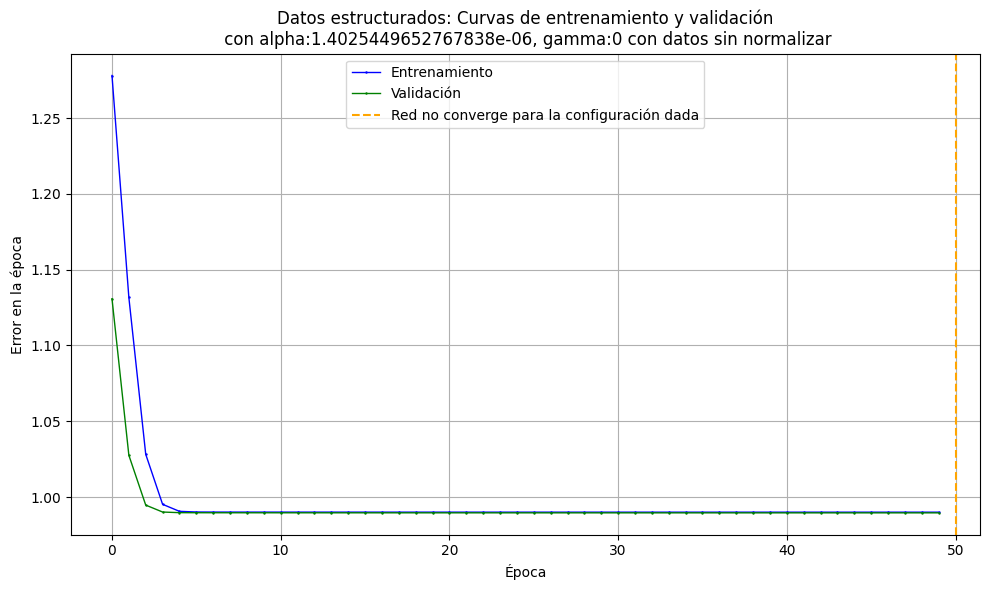
\includegraphics[width=\linewidth]{imgs/structured/basic.png}
        \caption{Gráficas de error con datos sin normalizar}
        \label{fig:basic}
    \end{subfigure}
    \hfill
    \begin{subfigure}{0.49\textwidth}
       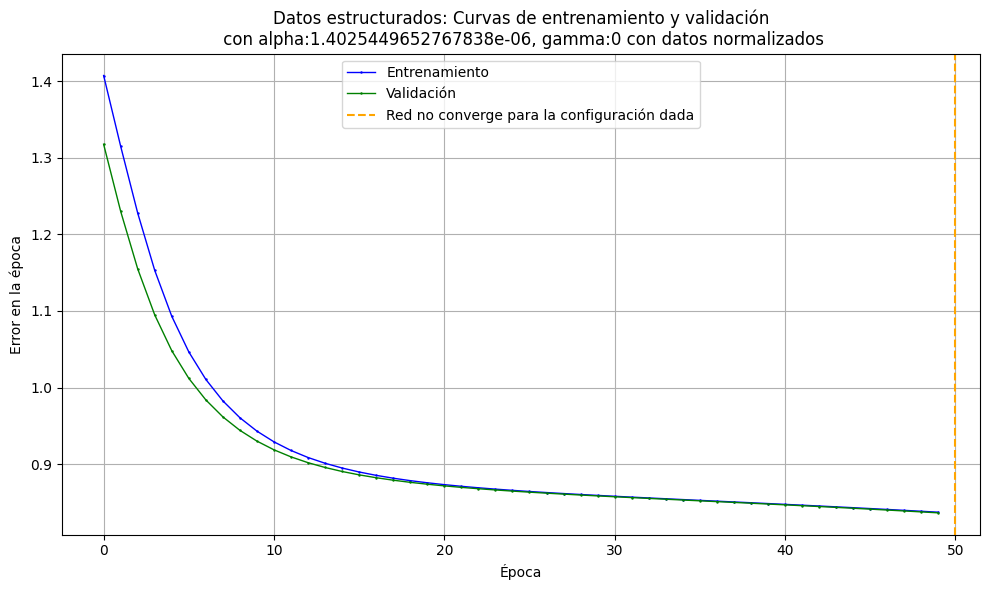
\includegraphics[width=\linewidth]{imgs/structured/normalized.png}
        \caption{Gráficas de error con datos normalizados}
        \label{fig:normalized}
    \end{subfigure}
    \caption{Comparativa de las curvas de error entre datos no normalizados y normalizados.}
    \label{fig:comparativa}
\end{figure}

De la anterior figura se puede evidenciar cómo al normalizar los datos, existe una mayor suavidad en las curvas de aprendizaje de los entrenamientos, así como una disminución en los errores:

\begin{figure}[htbp]
    \centering
    \begin{subfigure}{0.49\textwidth}
        \centering
        \begin{tabular}{rrr}
        \toprule
         Trial & min(training) & min(testing) \\
        \midrule
        30 & 0.990004 & 0.989558 \\
        \bottomrule
        \end{tabular}
        \caption{Errores con datos sin normalizar}
        \label{fig:basic}
    \end{subfigure}
    \hfill
    \begin{subfigure}{0.49\textwidth}
        \centering
       \begin{tabular}{lrrr}
        \toprule
        Trial & min(training) & min(testing) \\
        \midrule
        30 & 0.859436 & 0.858770 \\
        \bottomrule
        \end{tabular}

        \caption{Errores con datos normalizados}
        \label{fig:normalized}
    \end{subfigure}
    \caption{Comparativa de los errores entre datos no normalizados y normalizados.}
    \label{fig:comparativa}
\end{figure}

Nótese de la figura anterior como los datos normalizados presentan un menor error.

\newpage
\bibliographystyle{ieeetr}
\bibliography{referencias}

\end{document}
